%
%	filename:	docto.tex
%	contents:	博士論文
%	author:		1643002:門倉 強
%
%   序章 3ページ
%   論文要旨
%   量子流体 10ページ
%   古典流体と乱流 10ページ
%   量子流体と乱流 5ページ
%   乱流の統計則 5ページ
%   ランダム位相、ランダムポテンシャル 5ページ
%   「量子流体の渦度による階層構造」
%   序章 2ページ
%   方法 10ページ
%   結果
%   初期渦 20ページ
%   乱流  20ページ
%   考察 2ページ
%   「2次元3次元クロスオーバー」
%   序章 2ページ
%   方法 10ページ
%   結果 10ページ
%   考察 2ページ
%   まとめ 5ページ
%
%
\documentclass[12pt,a4paper]{jbook}
%\documentclass[12pt,a4paper]{jarticle}
%\documentclass[10pt,a4paper]{jbook}
%\documentclass[10pt,a4paper]{book}
%\documentclass[12pt,a4paper]{report} % 2014/09/27
%\documentclass[12pt,a4paper]{jarticle} % 2014/09/27
%\documentclass[10pt,a4paper]{jarticle} % 2014/09/27
%\documentclass[11pt,a4paper]{article} % 2014/09/27
%\documentclass[11pt,a4paper,twoside]{book} % 2014/09/27
%\documentclass[10pt,a4paper]{report}
%\documentclass[12pt,a4paper]{report} % 2014/11/30
%
%\if 0
\setlength{\oddsidemargin}{0mm}
\setlength{\evensidemargin}{0mm}
\setlength{\topmargin}{0mm}
\setlength{\headsep}{2truemm}
\setlength{\textwidth}{460pt}
%\setlength{\textheight}{750pt}
\setlength{\textheight}{22.80cm}
\setcounter{tocdepth}{2}
%\fi
%
\usepackage{amsmath,amssymb,bm}
%\usepackage{graphicx}
\usepackage[dvipdfmx]{graphicx}
\usepackage{cases}
\usepackage{ascmac}
%\usepackage{wasysym}
\usepackage{multicol}
\usepackage{mathrsfs}
\usepackage[scriptsize]{caption} % 2014/09/27
\usepackage{fancyhdr}
%\usepackage[dvipdfmx]{hyperref}
%\usepackage{showkeys}
%
\newcommand{\diff}{\mathrm{d}}				           %
\newcommand{\divergence}{\mathrm{div}\,}		       %
\newcommand{\grad}{\mathrm{grad}\,}			           %
\newcommand{\rot}{\mathrm{rot}\,}			           %
\newcommand{\const} {{\rm const.}}			           %
\newcommand{\h}  {{\rm h}}				               % プランク定数
\newcommand{\na} {N_{\rm A}}				           % アボガドロ定数
\newcommand{\kb} {k_{\rm B}}				           %
\newcommand{\me} {m_{\rm e}}				           %
\newcommand{\lap} {\bigtriangleup}			           %
\newcommand{\dal} {\Box}				               %
\renewcommand{\figurename}{FIG.}			           %
\def\Vec#1{\mbox{\boldmath $#1$}}			           %
\def\fourier#1 { {\cal F} \left\{ #1 \right\} }		   %
\def\ifourier#1 { {\cal F}^{-1} \left\{ #1 \right\} }  %
\def\laplace#1 { {\cal L} \left\{ #1 \right\} }		   %
\def\ilaplace#1 { {\cal L}^{-1} \left\{ #1 \right\} }  %
%
\title{
{\huge \tt
量子乱流における渦度の階層構造} \\
%{\Large 2021 The University of Electro-Communications \\
%Doctor's thesis} \\[1cm]
}
\author{
%\LARGE 学籍番号: \fbox{1643002} \\[0.5cm]
%\LARGE 氏名: \fbox{門倉 強} \\[0.5cm]
%\LARGE Department of Engineering Science \\[0.5cm]
%\LARGE SAITO Research Laboratory \\[0.5cm]
%\date{}
\\
\\
\\
\\
\LARGE 門倉 強
\\
\\
\\
\\
\\
\LARGE 電気通信大学 大学院 情報理工学研究科
\\
\\
\\
\\
\\
\LARGE 博士(理学)の学位申請論文
\\
\\
\\
\\
\Large 2020年12月
\\
\\
}
%
\input{jdummy.def} % October 20, 2018
%
\begin{document}
\maketitle


\makeatletter
\def\ps@fancy{%
%\def\sectionmark##1{\markboth{\ifnum \c@secnumdepth>\z@ \thesection\hskip 1em\relax \fi ##1}{}}%
\def\chaptermark##1{\markboth{\ifnum \c@secnumdepth>\z@ \thechapter\hskip 0.5em\relax \fi ##1}{}}%
%\def\subsectionmark##1{\markright {\ifnum \c@secnumdepth >\@ne \thesubsection\hskip 1em\relax \fi ##1}}%
\def\sectionmark##1{\markright {\ifnum \c@secnumdepth >\@ne \thesection\hskip 0.5em\relax \fi ##1}}%
\ps@@fancy
\gdef\ps@fancy{\@fancyplainfalse\ps@@fancy}%
\ifdim\headwidth<0sp
\global\advance\headwidth123456789sp\global\advance\headwidth\textwidth
\fi
}
\makeatother

\newpage
` 
\\
\\
\\
\\
\\
{\huge \tt
  量子乱流における渦度の階層構造
}
\\
\\
\\
\\
\\
\\
\\
\LARGE        博士論文審査委員会
\\
\\
\\
   主査  斎 藤  弘 樹 教授
\\
   委員  渡 辺  信 一 教授
\\
   委員  教授
\\
   委員  岸 本  哲 夫 准教授
\\
   委員  准教授
\newpage
\' 
\\
\\
\\
\\
\\
{\huge \tt
    著作権所有者
\\
\\
\\
\\
    門倉 強
\\
\\
     2020 年
}
\newpage
\normalsize
%\pagestyle{empty}
%\pagestyle{plain}
\pagestyle{fancy} % 2014/09/07
%\pagenumbering{roman}
\tableofcontents
\setcounter{page}{1}
\pagenumbering{arabic}
%\fancyhead[LE]{\thepage}  % 2014/09/07
%\fancyhead[RE]{\leftmark} % 2014/09/07
%\fancyhead[LO]{\leftmark} % 2014/09/07
%\fancyhead[RO]{\thepage}  % 2014/09/07
%\lhead{\thepage}
%\chead{}
%\rhead{\leftmark}
%\lfoot{} % 2014/09/07
%\cfoot{\thepage} % 2014/09/07
%\rfoot{} % 2014/09/07
%\chapter{イントロダクション}
%\chapter{ボース・アインシュタイン凝縮による量子流体}
%\chapter{量子乱流における渦度の階層構造}
%\section{目的}
%\section{方法}
%\section{結果}
%\chapter{二成分量子乱流におけるエネルギーカスケード}
%\section{目的}
%\section{方法}
%\section{結果}
%\chapter{量子乱流における二次元-三次元クロスオーバー}
%\section{目的}
%\section{方法}
%\section{結果}
\normalsize
巨視的なスケールをもつ超流動体における、量子乱流及び量子渦について
理論的に議論した。
粗視化した渦度分布を用いた研究がなされ、エネルギーカスケードの機構が
明らかにされた。一方、量子乱流においても、同様の機構によってエネルギー
カスケードが起こりKolmogorov則が表れていると期待される。
そこで我々は同様の手法を用いて量子乱流の研究を行った。


現象の超流動は広く研究がなされ
実験では。
理論では
その中で本論文では超流動体における乱流の理論的研究について述べる。
三次元乱流中のエネルギースペクトルの傾きは励起から散逸まで
一定の範囲で普遍性が認められ、一般的にコルモゴロフの-5/3乗則と称される。
量子流体においても同様の現象が確認されており、我々はこの波数空間における
コルモゴロフ則が実空間ではどのような物理現象に対応するか研究を進めた。

\ 目的
背景
方法
結果

\ We investigate quantum turbulence and quantized vortices in quanum fluids.


\ The Bose-Einstein condensation(BEC), that is one of the typical quantum phenomena,
is a phase transition.
In a Bose-Einstein condensate, a macroscopic number of
Bose particles occupy a single quantum state.
This phenomenon was predicted in 1924 by A.Einstein \cite{1} \cite{2}.
\ Einstein advanced Bose's idea and predicted that bosonic atoms or molecules
condense into a single wave function at low temperatures.
This theoretical prediction has been realized in 1995 \cite{3} \cite{4}.
\\
\ In 1908, helium was liquefied for the first time by Heike Kamerling Onness,
where the boiling point of helium is 4.2K.
Since then, characteristics of various substances at cryogenic temperature
were studied using liquid helium.
In particular, it was discovered in 1922 that the electrical resistance of mercury
disappeared at the helium temperature, which is called superconductivity.
%\\
%\ Satyendra Nath Bose generalized the papter on statistical description of the quanta of light in 1924 \cite{5} and A.Einstein \cite{6}.
\\
\ Willem Hendrik Keesom discovered in 1932 that there is a sharp peak
in the specific heat curve at the transition point 2.19K(normal pressure)
from helium I to helium II \cite{5}. Paul Ehrenfest named this phenomenon lambda transition,
since the curve was similar to the Greek symbol $\lambda$.
\\
\ In 1938, Pyotr Kapitza investigated the viscosity of liquid helium and
discovered that liquid helium flows in a capillary tube without viscosity \cite{6}.
This phenomenon is called superfluidity. Fritz Wolfgang London and Lev Davidovich Landau pioneered
in the theoretical investigation of superfluidity.
\\
\ F.London figured out that BEC is connected with
the $\lambda$-point phenomenon of liquid helium in 1938 \cite{7}.
\\
\ In 1961, Eugene Paul Gross and Lev Petrovich Pitaevskii derived Gross-Pitaevskii equation for the weak-interacting Bose-gas
\cite{8} \cite{9}.
\\ Afterward, it was experimentally investigated whether the superfluidity of helium is due to BEC in 1995\cite{10}\cite{11}\cite{12}.
It is difficult to compare experimental results with theoretical calculation.

\section{目的}
\ BEC like as dilute atomic gas condensation which has an inter-particle interaction
is the only object for which the essence of
these quantum phenomena can be pressed for many physicists.
Our purpose is to study them using numerical solutions.
We investigate dynamics in BEC.
This thesis aims to study phenomenon of the quantized vortex shedding
and critical velocity in Bose-Einstein condensates.

\section{構成}
\ 本論文の構成は以下の通りである。2章、3章では量子乱流、古典乱流の先行研究について、
4章では取り扱う超流動の定義、5章では本研究で用いるGross-Pitaevskii方程式、
パワースペクトル、ランダムポテンシャルについてのレビュー、
6章、7章では本研究での渦度の階層構造と、二次元三次元クロスオーバーについて述べる。
8章では以上の結果について述べる。


2章、3章では量子乱流、古典乱流の先行研究について
4章では我々が取り扱う超流動の定義、5章ではChapter 1 describes the background of this study.

\chapter{超流動体}

\section{量子流体}
\section{量子乱流}

\chapter{古典乱流}
\section{古典流体}
\section{古典乱流}

\chapter{超流動}

\chapter{方法}

\chapter{量子乱流における渦度の階層構造}

\chapter{量子乱流における二次元三次元クロスオーバー}

\chapter{まとめと展望}

\ The quantum property becomes significant, if particles are cooled.
The energy distribution of particles in thermal equilibrium obeys
the Bose-Einstein distribution or the Fermi-Dirac distribution \cite{13}\cite{14}.
\\
\ In the Fermi-Dirac distribution each quantum state is occupied only by a single particle.
By contrast, in the Bose-Einstein distribution each quantum state can be occupied by many particles.
\begin{figure}[htbp]
\begin{center}
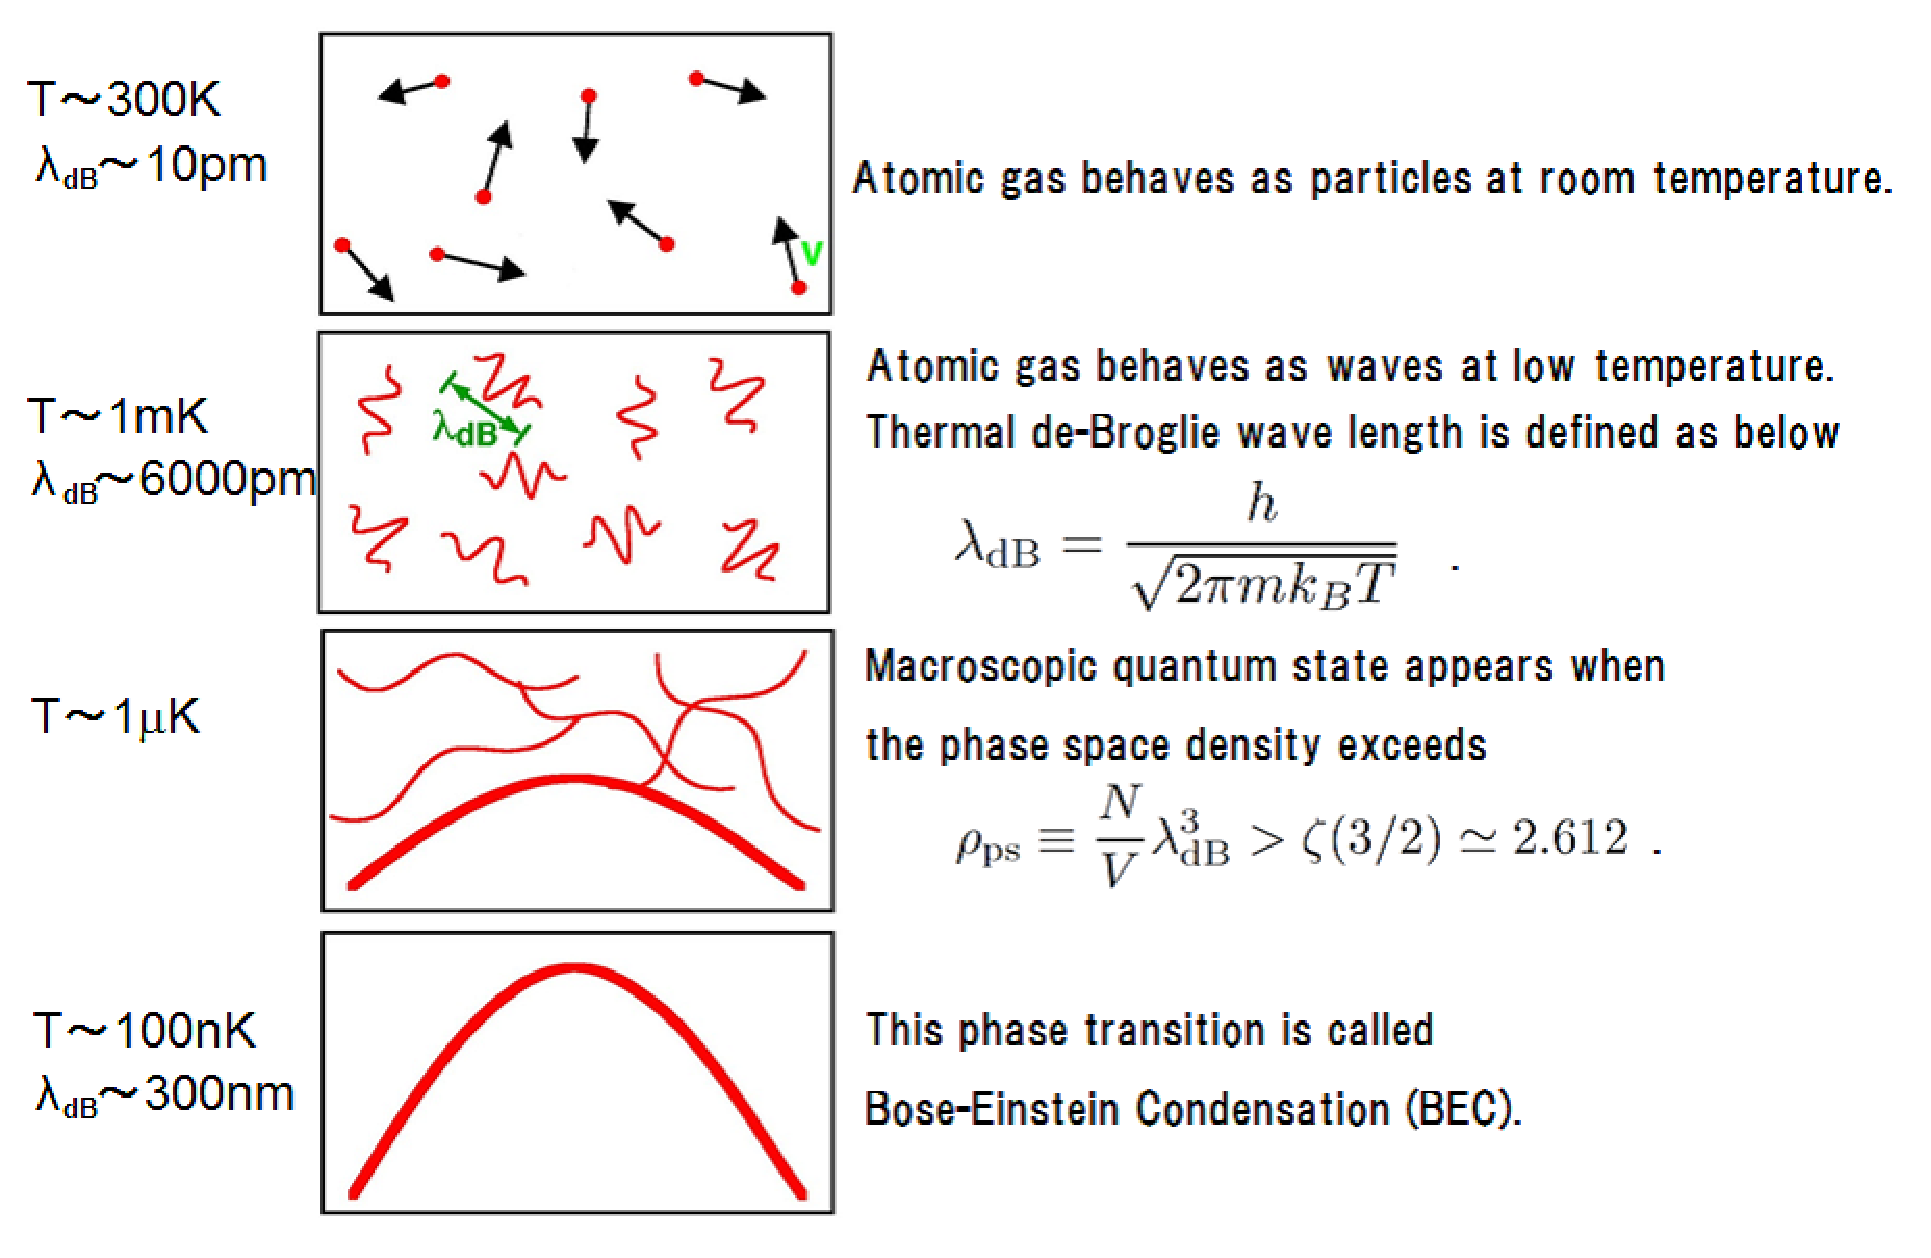
\includegraphics[scale=0.40, keepaspectratio]{2-1.eps}
\caption{
Schematic illustration of the BEC phase transition. \ $T$ is absolute temperature.
\ ${\lambda_{\rm dB}}$ is the de-Bloglie wavelength. \ $h$ is the Planck constant.
\ $m$ is atomic mass.
\ $\kb$ is Boltzmann constant. \ $\rho_{{\rm ps}}$ is the phase space density.
\ $N$ is number of atoms. \ $V$ is the volume of dilute atomic gas.\ $\zeta$ is the Riemann zeta function.
$\zeta(s)=\sum_{n=1}^\infty \frac{1}{n^s}$
}
\label{FIG:2-1}
\end{center}
\end{figure}

\section{古典流体と乱流}
\ Atoms can be classified into bose particles(boson) or fermi particles(fermion)
by total number of electrons, protons and neutrons.
$Z$ is the proton number and $N$ is the neutron number.Atomic mass number $A$ is
$A = Z + N$. Bose particles when $A$ is even and fermi particles when $A$ is odd.
Neutron number $N$ determine the statistics.
For example, Bose particles ${\rm ^{87}Rb}$ has an even neutron number $N = 50$.
Fermi particles ${\rm ^{40}K}$ has an odd neutron number $N = 21$.
\\
\ Fermions obey the Pauli exclusion principle \cite{15}.
The degeneracy pressure resists compression, which stabilizes white dwarf
and neutron stars.This is well known as the Chandrasekhar limit.
Bosons can occupy the same quantum state. The laser is a state, in which many bosons(photons)
occupy the same state.

\section{量子流体と乱流}
\ Number of ways to distribute $N_l$ bosons into $M_l$ states are given by
\begin{eqnarray}
W_l & = & _{M_l} {\rm H}_{N_l} = _{M_l + N_l - 1} {\rm C}_{N_l} =  \frac{(M_l+N_l-1)!}{(M_l+N_l-1-N_l)!N_l!}
,
\end{eqnarray}
where $l$ is the index of levels.
The total number of ways are therefore
\begin{eqnarray}
W_B[(N_l)] & = & \prod_l W_l = \prod_l \frac{(M_l+N_l-1)!}{N_l!(M_l+N_l-1-N_l)!}.
\end{eqnarray}
The entropy $S_B$ is defined by
\begin{eqnarray}
S_B[(N_l)] & \equiv & \kb \log W_B[(N_l)],
\end{eqnarray}
where $\kb$ is the Boltzman constant.Applying the Stirling formula, we have
\begin{eqnarray}
S_B[(N_l)] & = & \kb \sum_l \log
\left[
\frac{(M_l+N_l-1)!}{(M_l+N_l-1-N_l)!N_l!}
\right] \nonumber
\\
& = & \kb \sum_l M_l
\left[
\left(1 + \frac{N_l}{M_l}\right)
\log \left(1 + \frac{N_l}{M_l}\right)
- \frac{N_l}{M_l} \log \left( \frac{N_l}{M_l}\right)
\right].
\end{eqnarray}
Using the method of Lagrange multipliers,
\begin{eqnarray}
S^\prime [(N_l )] & = & S_B[( N_l )] - a \sum_l N_l - b \sum_l E_l N_l.
\end{eqnarray}
Partial derivative of $S^\prime [(N_l )]$ with respect to $N_l$ gives
\begin{eqnarray}
\frac{\partial}{\partial N_l}S^\prime [(N_l )] & = &
\kb
\left[
\log \left(1 + \frac{N_l}{M_l} \right) - \log \left( \frac{N_l}{M_l} \right)
\right] - a - b E_l = 0,
\end{eqnarray}
\begin{eqnarray}
\kb
\left[
\log \left(1 + \frac{N_l}{M_l} \right) - \log \left( \frac{N_l}{M_l} \right)
\right] & = & a + b E_l  \nonumber
\\
\log \left(1 + \frac{N_l}{M_l} \right) - \log \left( \frac{N_l}{M_l} \right)
& = & \frac{a + b E_l}{\kb}.
\end{eqnarray}
We define $\alpha \equiv \frac{a}{\kb}$ and $\beta \equiv \frac{b}{\kb}$, and Eq.(2.7) is written as
\begin{eqnarray}
\log \left(1 + \frac{N_l}{M_l} \right) - \log \left( \frac{N_l}{M_l} \right)
& = & \alpha + \beta E_l,
\\
\frac{1+\frac{N_l}{M_l}}{\frac{N_l}{M_l}} & = & e^{\alpha + \beta E_l} \nonumber
\\
\frac{M_l}{N_l} & = & e^{\alpha + \beta E_l} - 1 \nonumber
\\
\frac{N_l}{M_l} & = & \frac{1}{e^{\alpha + \beta E_l} -1}.
\end{eqnarray}
We define the total number of particles as using Eq.(2.9) the equation is
\begin{eqnarray}
N & \equiv & \sum_l N_l = \sum_l \frac{M_l}{e^{\alpha + \beta E_l} -1}.
\end{eqnarray}
Partial derivative of the entropy with respect to $N$ reads
\begin{eqnarray}
\left( \frac{\partial S}{\partial N} \right)_E & = &
\kb \sum_l (\alpha + \beta E_l) \left( \frac{\partial N_l}{\partial N} \right)_E,
\end{eqnarray}
\begin{eqnarray}
\sum_l \left( \frac{\partial N_l}{\partial N} \right)_E = 1,
\ \sum_l E_l \left( \frac{\partial N_l}{\partial N} \right)_E = 0.
\end{eqnarray}
Thus, we obtain
\begin{eqnarray}
\left( \frac{\partial S}{\partial N} \right)_E & = & \alpha \kb.
\end{eqnarray}
We define the total energy of particles as using Eq.(2.9) the equation is
\begin{eqnarray}
E & \equiv & \sum_l E_l N_l = \sum_l \frac{E_l M_l}{e^{\alpha + \beta E_l} -1}.
\end{eqnarray}
Partial derivative of the entropy with respect to $E$ yields
\begin{eqnarray}
\left( \frac{\partial S}{\partial E} \right)_N & = &
\kb \sum_l (\alpha + \beta E_l) \left( \frac{\partial N_l}{\partial E} \right)_N,
\end{eqnarray}
\begin{eqnarray}
& & \sum_l \left( \frac{\partial N_l}{\partial E} \right)_N = 0,
\ \sum_l E_l \left( \frac{\partial N_l}{\partial E} \right)_N = 1,
\end{eqnarray}
Therefore, we obtain
\begin{eqnarray}
\left( \frac{\partial S}{\partial E} \right)_N & = & \beta \kb.
\end{eqnarray}
From the thermodynamic relation, we get
\begin{eqnarray}
\alpha = - \frac{\mu}{\kb T}
, \ \beta & = & \frac{1}{\kb T},
\end{eqnarray}
where $\mu$ is a chemical potential. We thus obtain the Bose-Einstein distribution function for the energy state $\epsilon_{l=i}$ as
\begin{eqnarray}
\langle n_i \rangle & = & \langle n_{l=i} \rangle = \frac{N_i}{M_i} = \frac{1}{e^{\frac{\epsilon_i - \mu}{\kb T}} - 1}.
\end{eqnarray}

\section{乱流の統計理論}
\ We consider wavenumber space.
The average numbers of particles obey the Bose statistics given by
$\displaystyle \langle n_k \rangle = \frac{1}{e^{\frac{\epsilon_k - \mu}{\kb T}} - 1}$
and kinetic energy is $\displaystyle \epsilon_k = \frac{\hbar^2 k^2}{2 m}$,
 where the total number of particles $N$ is the sum of $\langle n_k \rangle$ as
\begin{eqnarray}
N & = & \sum_k \langle n_k \rangle
\\
& = & \langle n_0 \rangle  + \frac{V}{(2\pi)^3} \int_0^\infty 4 \pi k^2 \langle n_k \rangle \diff k  \nonumber
\\
& = & \langle n_0 \rangle + \left( \frac{L}{2\pi} \right)^3 \int_0^\infty 4 \pi k^2 \nonumber
\frac{1}{e^{\frac{\epsilon_k - \mu}{\kb T}} - 1} \diff k
\\
& = & N_0(T) + N^\prime(T),
\end{eqnarray}
where $\langle n_0 \rangle$ is the average number of particles in the ground state.
$N_0(T)$ is the number of particles in the ground state at temperature T.
We now consider the number of atoms in the excited states $N^\prime(T)$,
\begin{eqnarray}
N^\prime(T) & = & \left(\frac{L}{2 \pi}\right)^3 \int_0^\infty 4 \pi k^2
 \frac{1}{e^{\frac{\epsilon_k - \mu}{\kb T}} - 1}  \diff k.
\end{eqnarray}
The integral becomes largest energy, when the chemical potential $\mu=0$, then,
\begin{eqnarray}
N^\prime_{{\rm max}}(T) & \ge & \left(\frac{L}{2 \pi}\right)^3 \int_0^\infty 4 \pi k^2
 \frac{1}{e^{\frac{\hbar^2 k^2}{2 m} \cdot \frac{1}{\kb T}} - 1}  \diff k.
\end{eqnarray}
Using $u = \frac{\hbar^2 k^2}{2 m \kb T}$, the integral in Eq.(2.23) becomes dimensionless as
\begin{eqnarray}
\frac{N^\prime_{{\rm max}}(T)}{L^3} = n  & \ge & \left(\frac{1}{2 \pi} \right)^3 \cdot
4 \pi \cdot \frac{m \kb T}{\hbar^2} \cdot \frac{\sqrt{2 m \kb T}}{\hbar} \cdot
\int_0^\infty \frac{u^{1/2}}{e^u - 1} \diff u
\\
& \ge & 4 \pi \cdot \frac{m \kb T}{h^2} \cdot \frac{\sqrt{2 m \kb T}}{h} \cdot \Gamma \left( 1+\frac{1}{2}\right) \zeta \left( 1+\frac{1}{2}\right)  \nonumber
\\
& \ge & 4 \pi \cdot \frac{m \kb T}{h^2} \cdot \frac{\sqrt{2 m \kb T}}{h} \cdot \frac{\sqrt{\pi}}{2}\cdot \zeta \left( 1+\frac{1}{2}\right) \nonumber
\\
& \ge & \sqrt{8 \pi^3} \cdot \frac{\sqrt{m^2 \kb^2 T^2}}{h^2} \cdot \frac{\sqrt{m \kb T}}{h} \cdot \zeta \left( 1+\frac{1}{2}\right) \nonumber
\\
n & \ge & 2.612 \cdot \left( \frac{\sqrt{2 \pi m \kb T}}{h} \right)^{3}
= 2.612 \cdot \frac{1}{\lambda_{{\rm dB}}^3},
\end{eqnarray}
where we used the Gamma function and the Riemann zeta function.
Thus we obtain phase space density,
\begin{eqnarray}
\rho_{{\rm ps}} = n \lambda_{{\rm dB}}^3 & \ge & 2.612.
\end{eqnarray}

\section{Thermal de-Broglie wavelength in BEC}
In Eq.(2.25), thermal de-Broglie wavelength ($\lambda_{dB}$) plays an important in BEC.
At room temperature, $\lambda_{dB}$ is shorter than the atomic diameter.
As temperature decreases, $\lambda_{dB}$ becomes longer than atomic diameter.
Then the de-Broglie wavelength of each particle overlaps.
Whole particles begin to occupy a single energy state (ground state) and the many-body wave function
changes to a macroscopic wave function \cite{16}.We thus obtain
\begin{eqnarray}
\lambda_{\rm dB} & = & \frac{h}{\sqrt{2 \pi m \kb T}}.
\end{eqnarray}

\section{Phase transition temperature of BEC}
\ The BEC is a phenomenon, in which all particles fall in the minimum energy state.
We consider the case in which $N$ atoms with mass $m$ are contained with a volume $L^3$.
The eigenvalue $\epsilon_k$ of the kinetic energy is given by
\begin{eqnarray}
\epsilon_k = \frac{\hbar^2 k^2}{2m} = \frac{\hbar^2}{2m}(k_x^2+k_y^2+k_z^2).
\end{eqnarray}
We write the wavenumber vector as
\begin{eqnarray}
(k_x, k_y, k_z) & = & \frac{2 \pi}{L}(n_x, n_y, n_z),
\end{eqnarray}
where $n_x,n_y,n_z = 0, 1, 2, \cdots$ .
Subtracting the number of atoms in the ground state $N_0$ from the total number of atoms $N$,
we have the number of excited atoms as
\begin{eqnarray}
N - N_0 = \sum_{k \neq 0} \frac{1}{ e^{\beta (\epsilon_k - \mu)} - 1},
\end{eqnarray}
where $\beta = 1/(\kb T)$.
Replacing the summation with an integral approximation for a large system as
\begin{eqnarray}
\frac{1}{V} \sum_{k \neq 0} & \rightarrow & \int \frac{\diff^3 k}{(2 \pi)^3}.
\end{eqnarray}
At temperature $T$, expectation value of the number atoms in $k$ state
with an energy $\epsilon_k$ is calculated as
\begin{eqnarray}
\langle n_k \rangle & = & \frac{1}{e^{\frac{\epsilon_k - \mu}{\kb T}} - 1},
\end{eqnarray}
where $\mu \leq 0$. The chemical potential $\mu$ is determined in
such a way that $N = \sum_k \langle n_k \rangle$.
The total number of atoms then becomes
\begin{eqnarray}
N & = & \sum_k \frac{1}{e^{\frac{\epsilon_k - \mu}{\kb T}} - 1}.
\end{eqnarray}
We replace the summation with the integration using the density of state,
\begin{eqnarray}
N & = & \int_{-\infty}^{\infty} \frac{ D(\epsilon)}{e^{\frac{\epsilon_k - \mu}{\kb T}} - 1}  \diff \epsilon.
\end{eqnarray}
We define the density of states
\begin{eqnarray}
D(\epsilon) & \equiv & 2 \pi V \left( \frac{2m}{\hbar^2} \right)^{\frac{3}{2}} \sqrt{\epsilon}.
\end{eqnarray}
Using the de-Broglie wavelength
\begin{eqnarray}
\lambda_{\rm dB} & = & \frac{\hbar}{\sqrt{2 \pi m \kb T}},
\end{eqnarray}
Equation (2.30) is shown to be
\begin{eqnarray}
N - N_0 & = & \frac{V}{\lambda_{\rm dB}^3} b_{3/2} (z).
\end{eqnarray}
Where the function $b_{n}(z)$ is the Bose-Einstein integration,
\begin{eqnarray}
b_n (z) & = & \frac{1}{\Gamma (n)} \int_0^\infty \frac{x^{n-1}}{e^{\frac{x}{z}}-1} \diff x.
\end{eqnarray}
At high temperature, the right-hand side of Eq.(2.37) is of order of N. However at low temperature,
$N_0$ is much smaller than $N$.
Then, Eq.(2.37) with $N_0 = 0, \mu = 0$ becomes as
\begin{eqnarray}
b_{\frac{3}{2}}(z) \leq b_{\frac{3}{2}}(1) = \zeta \left( \frac{3}{2} \right) = 2.6128 \cdots.
\end{eqnarray}
At low temperature, in the right-hand side of Eq.(2.37),
the number of atoms in the ground state, $N_0$ becomes dominant T, giving
\begin{eqnarray}
N & = & \frac{V}{\lambda_{\rm dB}^3 b_{\frac{3}{2}} }(1).
\end{eqnarray}
We obtain the critical temperature $T_c$
\begin{eqnarray}
T_c & = &
\left[ \zeta \left( \frac{3}{2} \right) \right]^{-\frac{2}{3}} \frac{2 \pi \hbar^2}{m \kb} \left( \frac{N}{V} \right)^{\frac{2}{3}}.
\end{eqnarray}

\section{Off-diagonal long-range order (ODLRO)}
\ We consider the ideal Bose particles in the energy state $k$ with three dimensional wavenumber space.
Annihilation and creation operators are defined by $\hat{a}_{k}$ and $\hat{a}^\dagger_{k}$.
The number of particles in the state with wavenumber $k$ denoted by $n_k$. They satisfy
\begin{eqnarray}
\hat{a}_k | n_k \rangle & = & \sqrt{n_k}|n_k - 1 \rangle,
\\
\hat{a}^\dagger_k | n_k \rangle & = & \sqrt{n_k+1} | n_k + 1 \rangle,
\\
\left[ \hat{a}_k, \hat{a}^\dagger_k \right] & = & \delta_{k,k^\prime},
\\
\left[ \hat{a}_k, \hat{a}_k \right] & = & \left[ \hat{a}^\dagger_k, \hat{a}^\dagger_k \right] = 0.
\end{eqnarray}
\ Statistical average of number operator $\langle \hat{n}_k \rangle$
is according to the Bose distribution,
\begin{eqnarray}
n_k & = & \langle \hat{n}_k \rangle = \langle \hat{a}^\dagger_k \hat{a}_k \rangle = \frac{1}{e^{\beta(\epsilon_k - \mu)} - 1},
\end{eqnarray}
where $\beta = 1/\kb T$,
We define the Bose field operator $\psi$ using the creation and annihilation operators,
\begin{eqnarray}
\left \{
\begin{array}{l}
\hat{\psi} (r) = \frac{1}{\sqrt{V}} \sum_K e^{i k \cdot r} \hat{a}_k
\\
\\
\hat{\psi}^\dagger (r) = \frac{1}{\sqrt{V}} \sum_K e^{-i k \cdot r} \hat{a}^\dagger_k
\end{array}
\right.
\end{eqnarray}
Then, the commutation relation fulfills
\begin{eqnarray}
\left[ \hat{\psi}(\vec{r}), \hat{\psi}^\dagger(\vec{r}^{\ \prime} ) \right] & = & \delta( \vec{r} - \vec{r}^{\ \prime} )
\\
\left[ \hat{\psi}(\vec{r}), \hat{\psi}(\vec{r}^{\ \prime} ) \right] & = &
\left[ \hat{\psi}^\dagger(\vec{r}), \hat{\psi}^\dagger(\vec{r}^{\ \prime} ) \right] = 0
\end{eqnarray}
We write the momentum $p=0$ consistent in the Bose field as $\psi_0$,
\begin{eqnarray}
\left \{
\begin{array}{l}
\hat{\psi}(\vec{r}) = \psi_0 + \frac{1}{\sqrt{V}} \sum_{k \neq 0} e^{i k \cdot r} \hat{a}_k,
\\
\\
\hat{\psi}^\dagger(\vec{r}) = \psi^\dagger_0 + \frac{1}{\sqrt{V}} \sum_{k \neq 0} e^{-i k \cdot r} \hat{a}^\dagger_k,
\end{array}
\right.
\end{eqnarray}
where the classical field $\psi_0 ( \vec{r} )$ is called the wave function of the condensate.
The commutation relation fulfills
\begin{eqnarray}
\left[ \psi_0, \psi^\dagger_0 \right] & = & V^{-1} \left[ \hat{a}_k, \hat{a}^\dagger_k \right]
= V^{-1} \rightarrow 0.
\end{eqnarray}
We define the correlation function for an ideal the Bose particle system,
\begin{eqnarray}
\rho( \vec{r}, \vec{r}^{\ \prime} ) & \equiv & \langle \hat{\psi}^\dagger(\vec{r}^{\ \prime}) \hat{\psi}( \vec{r} ) \rangle.
\end{eqnarray}
If $\vec{r} = \vec{r}^\prime$, the function becomes the expectation value of the density operator.
In a homogeneous system, the density $\rho$ is the function of $\vec{r} - \vec{r}^\prime$.
We can write the correlation function, using Eq.(2.50),
\begin{eqnarray}
\rho( \vec{r} - \vec{r}^{\ \prime} ) & = & \langle \psi^\dagger_0 \psi_0 \rangle
+ \frac{1}{\hbar^3} \int \diff k \frac{e^{i k  (\vec{r} - \vec{r}^{\prime})}}
{e^{\beta (\epsilon_{\vec{k}} - \mu)} - 1}.
\end{eqnarray}
The first term of the right-hand side shows long range correlation, since
it is independent if $\vec{r}$ and $\vec{r}^\prime$, which indicates the density of the condensate.
On the other hand, the second term of the right-hand side shows short range correlation,
since it decays for large $\vec{r} - \vec{r}^\prime$.
If there is the interaction, we write
%the correlation function is
%\begin{eqnarray}
%\rho( \vec{r}, \vec{r}^{\ \prime} ) & = &  \langle \psi^\dagger( \vec{r}^{\ \prime} ) \psi (\vec{r}) \rangle,
%\\
%& = & \langle \psi^\dagger( \vec{r}^{\ \prime} ) \rangle \langle \psi (\vec{r}) \rangle + C ( \vec{r}, \vec{r}^{\ \prime} ).
%\end{eqnarray}
%where the first term of the right hand side means long range correlation, and the second term means short range
%correlation. Furthermore,
%if we write
\begin{eqnarray}
\varPsi( \vec{r} ) = \langle \hat{\psi}(\vec{r}) \rangle, \ \varPsi^*( \vec{r} ) = \langle \hat{\psi}^\dagger(\vec{r}) \rangle,
\end{eqnarray}
the part of long range correlation is written %the off diagonallike
as
\begin{eqnarray}
\varPsi^*(\vec{r}^\prime) \varPsi(\vec{r}) = |\psi(\vec{r})|^2.
\end{eqnarray}
Therefore, it is called the off-diagonal long-range order.
%And the $\Psi(\vec{r})$ is normaly $0$ quantity because of the expectation number
%is one particle annihilation operator.

\section{Gross-Pitaevskii equation}
We consider the Bose particles confined in a potential $V(\vec{r})$.
The many-body Hamiltonian is given by
\begin{eqnarray}
\mathcal{H} & = & - \int \diff \vec{r} \hat{\psi}^\dagger (\vec{r}) \left (\frac{\hbar^2}{2m} \nabla^2 \right)
\hat{\psi}(\vec{r}) \nonumber
\\
& & + \frac{1}{2} \int \int \diff \vec{r} \diff \vec{r}^{\ \prime} \hat{\psi}^\dagger( \vec{r} ) \hat{\psi}^\dagger( \vec{r}^{\ \prime} )
V (\vec{r} - \vec{r}^{\ \prime} ) \hat{\psi}( \vec{r}^{\ \prime} ) \hat{\psi}( \vec{r} ).
\end{eqnarray}
The interaction is approximated by the Fermi contact type interaction as
\begin{eqnarray}
V (\vec{r} - \vec{r}^{\ \prime} ) = g \delta (\vec{r} - \vec{r}^{\ \prime}),
\end{eqnarray}
where  $g = \frac{4 \pi \hbar^2 a}{m}$
%, \ \vec{r}^{\ \prime}$ is displacement from $\vec{r}$
and $a$ is the $s$-wave scattering length.
\\
Applying the Heisenberg equation of motion, we find
\begin{eqnarray}
i \hbar \frac{\partial}{\partial t} \hat{\psi} ( \vec{r}, t ) & = & \left[ \hat{\psi} ( \vec{r}, t ), \mathcal{H} \right] \nonumber
\\
& = & - \left( \frac{\hbar^2}{2m} \nabla^2 \right) \hat{\psi} ( \vec{r}, t )
+ g \hat{\psi}^\dagger (\vec{r}, t) \hat{\psi}( \vec{r}, t) \hat{\psi}( \vec{r}, t ).
\end{eqnarray}
Replacing the field operator $\hat{\psi}(\vec{r},t),\hat{\psi}^\dagger(\vec{r},t)$ with the c-number function
$\psi(\vec{r},t),\psi^\dagger(\vec{r},t)$,
%The field operator $\hat{\psi} (\vec{r})$ that annihilates a particle at the position $\vec{r}$ can be written
%in the form
%\begin{eqnarray}
%\psi( \vec{r} ) = \sum_i \varphi_i (\vec{r}) \hat{a}_i,
%\end{eqnarray}
%The c-number wavefunction $\psi$ satisfices an orthonormal condition
%\begin{eqnarray}
%\int \varphi^*_i( \vec{r}) \varphi_j( \vec{r}) \diff \vec{r} & = & \delta_{ij}.
%\end{eqnarray}
\\
we thus obtain the Gross-Pitaevskii equation \cite{17}.
\begin{eqnarray}
i \hbar \frac{\partial}{\partial t} \psi ( \vec{r}, t ) & = &
- \left( \frac{\hbar^2}{2m} \nabla^2 \right) \psi( \vec{r}, t)
+ g | \psi(\vec{r}, t) |^2 \psi( \vec{r}, t )
\end{eqnarray}
\if 0
\begin{eqnarray}
E & = & \frac{\hbar^2}{2m} ||\nabla \psi^2|| + V |\psi|^2 + g \frac{|\psi|^4}{2}
\\
L & = & T - E
\\
& = & \frac{i \hbar (\bar{\psi}\partial \psi/\partial t - \psi \partial \bar{\psi} / \partial t)}{2}
- \frac{\hbar^2}{2m} ||\nabla \psi^2|| - V |\psi|^2 - g \frac{|\psi|^4}{2}
\end{eqnarray}
\begin{eqnarray}
\hat{H} & = & \sum_i^N \left[ - \frac{\hbar^2}{2M} \nabla_i^2 + V (\vec{r}_i) \right] + U \sum_{i>j}
\delta(\vec{r}_i - \vec{r}_j)
\\
U \sum_{i>j} \delta(\vec{r}_i - \vec{r}_j)
\\
U = \frac{4 \pi \hbar^2 a}{M}
\end{eqnarray}
\fi
\section{Bogoliubov sound speed}
\ We now consider the sound velocity for investigating the critical velocity in the BEC.
We start from the Bogoliubov dispersion relation.
We assume the case in which Bose particles in the BEC interact with each other by repulsive potential.
This interaction associates small-energy and long-wavelength fluctuations in the condensate.
To investigate them, we begin with the Gross-Pitaevskii equation for the order parameter,
\begin{eqnarray}
i \hbar \frac{\diff}{\diff t} \psi(r,t) & = & \left[ - \frac{\hbar^2}{2m} \nabla^2 + g | \psi(r,t) |^2 \right] \psi(r,t),
\end{eqnarray}
where $g>0$ is a repulsive interaction parameter.
We assume that the solution of Eq.(2.60) is expanded as
\begin{eqnarray}
\psi(r,t) & = & \psi_0(r)e^{-i \mu t} +
\sum_k \left\{
u_k e^{i[kr - (\mu + \omega)t]} + v_k e^{-i[kr - (\mu + \omega)t]}
\right\},
\end{eqnarray}
where $u_k(r)$ and $v_k(r)$
are the excitation amplitudes % of forward propagating and backward propagating
waves with wavenumber $\pm k$. Substituting Eq.(2.61) into Eq.(2.60),
we obtain the eigenvalue equations for the two excitation waves.
\begin{eqnarray}
\left(
\begin{array}{c c}
\frac{\hbar^2 k^2}{2m} + \mu & \mu
\\
-\mu & -\frac{\hbar^2 k^2}{2m} - \mu
\end{array}
\right)
\left(
\begin{array}{c}
u_k
\\
v_k
\end{array}
\right)
& = &
\hbar \omega
\left(
\begin{array}{c}
u_k
\\
v_k
\end{array}
\right),
\end{eqnarray}
where $\hbar \mu = \hbar g|\psi_0(r)|^2 = \hbar gn_0$ is a chemical potential.
The eigenvalues $\omega$ of Eq.(2.62) is obtained by
\begin{eqnarray}
\hbar \omega^2 - \left(
\mu + \frac{\hbar^2 k^2}{2m}
\right)^2
+ \mu^2 & = & 0.
\end{eqnarray}
We get the solution of Eq.(2.63) as follows,
\begin{eqnarray}
\hbar \omega & = & \pm \sqrt{\omega_k (\omega_k + 2\mu)},
\end{eqnarray}
where
\begin{eqnarray}
\hbar \omega_k & = & \frac{(\hbar k)^2}{2m}
\end{eqnarray}
is the kinetic energy of a non-interacting free particle.
\\
%Then, the wavenumber takes the limit of zero
Taking the limit of $k \rightarrow 0$, we find
\begin{eqnarray}
\lim_{k \rightarrow 0} \hbar \omega_k & = & \lim_{k \rightarrow 0} \pm \sqrt{\frac{(\hbar k)^2}{2m} \left( \frac{(\hbar k)^2}{2m} + 2\mu \right)},
\\
& \simeq & \pm \sqrt{\frac{(\hbar k)^2}{2m} 2 g n} = \pm \hbar k \sqrt{\frac{gn_0}{m}}.
\\
|\omega_k| & \simeq & k \sqrt{\frac{gn_0}{m}}.
\end{eqnarray}
This has a linear dispersion relation as
\begin{eqnarray}
\omega_k & = & \pm v_s k,
\end{eqnarray}
where $v_s$ is the sound velocity for the long-wavelength,
\\
%Substitute Eq.(2.87) for Eq.(2.86)
\begin{eqnarray}
v_s & = & \sqrt{\frac{g n_0}{m}}.
\end{eqnarray}
Thus, we obtain the Bogoliubov sound speed \cite{18}.
%
%We define the healing length as
%\begin{eqnarray}
%\xi & \equiv & \sqrt{\frac{\hbar}{m \mu}}.
%\end{eqnarray}

\if 0
\section{Velocity field of superfluidity with super macroscopic wave function}
\ We consider the macroscopic wave function
\begin{eqnarray}
\psi(\vec{r}) = \sqrt{n(\vec{r})} e^{i \phi(\vec{r})}
\end{eqnarray}
The momentum density $j$ is given by
\begin{eqnarray}
j & = & - \frac{i \hbar}{2m} \left( \psi^* \nabla \psi - \psi \nabla \psi^* \right) = \frac{\hbar}{m} n_0 \nabla \phi.
\end{eqnarray}
Substituting Eq.(2.72) into Eq.(2.73),
we obtain the velocity of the condensate is defined by
\begin{eqnarray}
v_{s} & \equiv & \frac{j}{n_0} = \frac{\hbar}{m} \nabla \phi.
\end{eqnarray}
Therefore the phase transition is according to the flow of the superfluid.
\fi

\section{Quantized Vortex}
%\ The nonuniform dilute Bose gas consists of non-interacting atoms.
From Equation (2.55) $|\psi(\vec{r})|^2$ indicates the density of condensed atoms.
\\
\ We define the order parameter as
\begin{eqnarray}
\psi( \vec{r} ) & \equiv & \sqrt{\rho(\vec{r})} e^{i \theta(\vec{r})},
\end{eqnarray}
where $\rho$ is the density in the ground state and $\theta$ is the phase.
From the Gross-Pitaevskii(GP) equation and Eq.(2.71), we can derive the equation of continuity as
\begin{eqnarray}
\frac{\partial \rho}{\partial t} & = & \frac{i \hbar}{2m} \nabla \cdot ( \psi^* \nabla \psi - \psi \nabla \psi^* ),
\end{eqnarray}
where
\begin{eqnarray}
\vec{j} & = &  \rho \left( \frac{\hbar}{m} \nabla \phi \right) = \rho \vec{v},
\end{eqnarray}
with
\begin{eqnarray}
\vec{v} & = & \frac{\hbar}{m} \nabla \phi.
\end{eqnarray}
We define the circulation
\begin{eqnarray}
\Gamma \equiv \oint_c \vec{v} \cdot \diff \vec{r} = \frac{\hbar}{m} 2 \pi n = \frac{h}{m} n
\end{eqnarray}
where $n$ is an integer called the  quantum number of a vortex.
We find that the circulation in Eq.(2.75) is quantized in unit of $h/m$.
This mechanism is called the vortex quantization.

\if 0 %/* 20150104 */
\begin{eqnarray}
\Gamma & \equiv & \oint_c \vec{c} \cdot \diff \vec{r} = n \frac{\hbar}{m} 2 \pi = n \frac{h}{m}
\end{eqnarray}
where $n$ is integer quantum number.
Now we consider cylindrical coordinate.
\begin{eqnarray}
\psi(r, \theta, z) & = & e^{i n \theta}|\psi(r, \theta, z)|
\end{eqnarray}
\begin{eqnarray}
v_s & = & \frac{n}{2 \pi r}\frac{h}{m}
\end{eqnarray}
The term of the kinetic energy is given by
\begin{eqnarray}
- \frac{\hbar^2}{2m} \nabla^2 \psi & = & -\frac{\hbar^2}{2m}
\left[ \frac{\partial^2}{\partial r^2} + \frac{1}{r} \frac{\partial}{\partial r}
+ \frac{1}{r^2}\frac{\partial^2}{\partial \theta^2} + \frac{\partial^2}{\partial z^2}
\right] \psi
\end{eqnarray}
The term of $\theta$ is given by
\begin{eqnarray}
-\frac{\hbar^2}{2mr^2} \frac{\partial^2}{\partial \theta^2} \psi
& = & \frac{\hbar^2 n^2}{2mr^2} \psi \equiv U_{ef} \psi
\end{eqnarray}
where $U_{ef}$ is called the centrifugal potential which works the leaving force from origin.


\section{Bogoliubov Excitation Spectrum}
\ We are able to investigate an excitation spectrum represents spatial phase modulation of BEC
by using the Bogoliubov equations.

\section{Bogoliubov Sound Speed}
\ Sound speed is significant parameter.Vortex shedding is due to it in BEC
Sound speed can derive by the Bogoliubov dispersion relation.
\begin{eqnarray}
(\hbar \omega)^2 & = & \frac{\hbar^2 k^2}{2m} \left( \frac{\hbar^2 k^2}{2m} + 2 g n \right)
\end{eqnarray}
\begin{eqnarray}
\psi(\vec{r}, t) & = & \psi_0 (\vec{r}) e^{-i \mu t}
+ \psi_k e^{i \left[ \vec{k} \cdot \vec{r} - (\mu + \omega) t \right]}
+ \psi_{-k} e^{-i \left[ \vec{k} \cdot \vec{r} - (\mu - \omega) t \right]}
\end{eqnarray}
\begin{eqnarray}
\mu & = & g \psi^2_0 = 2gn_0
\end{eqnarray}
\begin{eqnarray}
(\mu + \omega) \psi_{k} & = & \frac{\hbar^2 k^2}{2m} \psi_{k} + \mu(2 \psi_{k} \psi_{-k} )
\\
(\mu - \omega) \psi_{-k} & = & \frac{\hbar^2 k^2}{2m} \psi_{-k} + \mu(2 \psi_{-k} \psi_k )
\end{eqnarray}
\begin{eqnarray}
\left[ A \right]
\left( \begin{array}{c} \psi_k \\ \psi_{-k} \end{array} \right)
& = &
\left( \begin{array}{c c}
\frac{\hbar^2 k^2}{2m} + \mu & \mu
\\
-\mu & \frac{\hbar^2 k^2}{2m} - \mu
\end{array} \right)
\left( \begin{array}{c} \psi_k \\ \psi_{-k} \end{array} \right)
=
\omega
\left( \begin{array}{c} \psi_k \\ \psi_{-k} \end{array} \right)
\\
{\rm Det} \left[A - \omega I \right] & = & 0
\end{eqnarray}
\fi %/* 20150104 */

\chapter{量子乱流における渦度の階層構造}
\section{序章}
\ In this chapter, the critical velocity defines the limit of no vortex shedding.
By numerically solving the Gross-Pitaevskii(GP) equation,
we show vortex pairs are formed in the wake of an obstacle potential moving in a BEC.
Mean-field analysis of systems of a BEC with a moving potential has been performed by
many authors from the viewpoints of drag force \cite{19}\cite{20}\cite{21}, vortex dynamics near the cylinder \cite{22}\cite{23},
critical velocity \cite{24}, scaling laws \cite{25}, supersonic flows \cite{26}\cite{27}, and multi-component systems \cite{28}\cite{29}.
In this paper, we investigate to aim the critical velocity for vortex shedding.
\\
\ When a cylindrical obstacle is moved in a viscous fluid with an appropriate velocity,
vortices are beginning shed in the wake.
The vortex are observed in a wide scale throughout nature: from a bathtub to
the atmosphere on a planet.
\ The behaviors are not only a classical viscous fluid past an obstacle but also superfluids,
in which viscosity is absent and a vortex is quantized. This prediction has been made by
numerical simulations of the GP equation, and therefore the phenomenon
can be observed in the systems that are described by the GP equation, such as an atomic-gas
Bose-Einstein condensate \cite{30} and an exciton-polariton superfluid in a
semiconductor microcavity \cite{31}\cite{32}. Theoretical studies on the dynamics of superfluids behind a
moving obstacle have been performed by many researchers

\section{方法}
\ We consider a BEC of atoms with mass $m$ and an obstacle potential $V$
moving in the $-x$ direction at a velocity $v$. In the mean-field theory,
the condensate is described by the macroscopic wave function $\psi$ obeying
the GP equation given by
\begin{eqnarray}
i \hbar \frac{\partial \psi}{\partial t} & = &
- \frac{\hbar^2}{2m} \nabla^2 \psi + V \psi + g | \psi |^2 \psi,
\end{eqnarray}
where $\displaystyle g = \frac{4 \pi \hbar^2 a}{m}$ with $a$ begin the
$s$-wave scattering length of the atoms. We employ a binary potential with
peak strength $V_0$ and radius $d$ moving in the $-x$ direction
at a velocity $v$ as $V = V_0 e^{-\frac{(x+\vec{v}t)^2+y^2}{d^2}}$.
\\
\begin{eqnarray}
V( \vec{r}, t ) & = & V_0 exp
\left\{
- \left[
\vec{r} - \vec{r}_{{\rm pot}} (t)
\right]^2 /d^2
\right\},
\end{eqnarray}
where $V_0$ is the peak intensity, $x$ is the position of the center, and $d$ is the $1/e$ width.
For an atomic Bose-Einstein condensate, such a potential can be produced by a blue-detuned $V_0 > 0$
Gaussian laser beam.In the present study, we consider the case of $V_0 > 0$.
The vortex generation dynamics for $V_0 < 0$ has been studied in Ref.[33].
\begin{eqnarray}
\vec{r} (t) & = & - v t \hat{x} + \hat{y},
\end{eqnarray}
where $\hat{x}$ and $\hat{y}$ are the unit vectors, $v > 0$ is the velocity in the $-x$ direction,
and $a$ and $\omega$ are the amplitude and frequency of the potential.
\\
\ We numerically solve Eq.(3.1) using the pseudo-spectral method[34]. The initial state is the ground state
of Eq.(3.1) with the initial position of the Gaussian potential, which is obtained by the
imaginary-time propagation method.The norm of the wave function, $\int |\Psi|^2 \diff \vec{r}$, is
chosen such that the density $n_0$ far from the obstacle potential becomes a desired value.
To break the exact numerical symmetry, small white noise is added to the initial state.
We take a large enough space and the boundary condition does not affect the result.
\ The characteristic length scale of the system is the healing length defined by
$\xi = \hbar(mg n_0)^{1/2}$. The sound velocity for the uniform density
$n_0$ is $v_s =(g n_0 / m)^{1/2}$ . The characteristic time scale and energy are
defined as $\tau = \hbar/(g n_0)$ and $\mu = g n_0$, respectively.
For a typical experimental system of an atomic Bose-Einstein condensate, $\xi \sim 0.1 {\rm \mu m},
v_s \sim 1 {\rm mm/s},$ and $\tau \sim 0.1 {\rm ms}$. For an exciton-polariton
superfluid in a semiconductor microcavity, $\xi \sim 1 {\rm \mu m}, v_s \sim 10^6 {\rm m/s},$
and $\tau \sim 1 {\rm ps}$[32].
\\
\ The GP equation in Eq.(3.1) has a scaling property. Normalizing the length, time and density
by $\xi,\tau,$ and $n_0,$ respectively, we can eliminate the interaction coefficient $g$
from the equation as
\begin{eqnarray}
i \frac{\partial \tilde{\psi}}{\partial \tilde{t}}
& = & -\frac{1}{2} \tilde{\nabla}^2 \tilde{\psi} + \tilde{V} \tilde{\psi} + |\tilde{\psi}|^2 \tilde{\psi},
\end{eqnarray}
where tildes are put to the normalized quantities, The independent parameters are therefore
$V_0, d, v, a,$ and $\omega$.
When $V_0$ is much larger than the chemical potential $\mu$, a circular hard-wall potential
with an effective radius $R$, given by
\begin{eqnarray}
V_0 e^{-R^2/d^2} \simeq \mu.
\end{eqnarray}
\begin{eqnarray}
\psi = \sqrt{n} e^{i \theta}
\end{eqnarray}
\begin{eqnarray}
i \hbar \frac{\partial \psi}{\partial t} & = & -\frac{\hbar^2}{2m} \nabla^2 \psi + g | \psi |^2 \psi
\end{eqnarray}
\begin{eqnarray}
\left \{
\begin{array}{l}
\displaystyle \hbar \frac{\partial \sqrt{n}}{\partial t} = - \frac{\hbar^2}{2m} \left[ 2 \left(\nabla \theta \right) \cdot \left( \nabla \sqrt{N} \right) + \left( \nabla^2 \theta \right) \sqrt{n} \right]
\\
\\
\displaystyle -\hbar \sqrt{n} \frac{\partial \theta}{\partial t} = - \frac{\hbar^2}{2m} \left[ \nabla^2 \sqrt{n} - \sqrt{n} \left( \nabla \theta \right)^2 \right] + gn \sqrt{n}
\end{array}
\right.
\end{eqnarray}
\begin{figure}[htbp]
\begin{center}
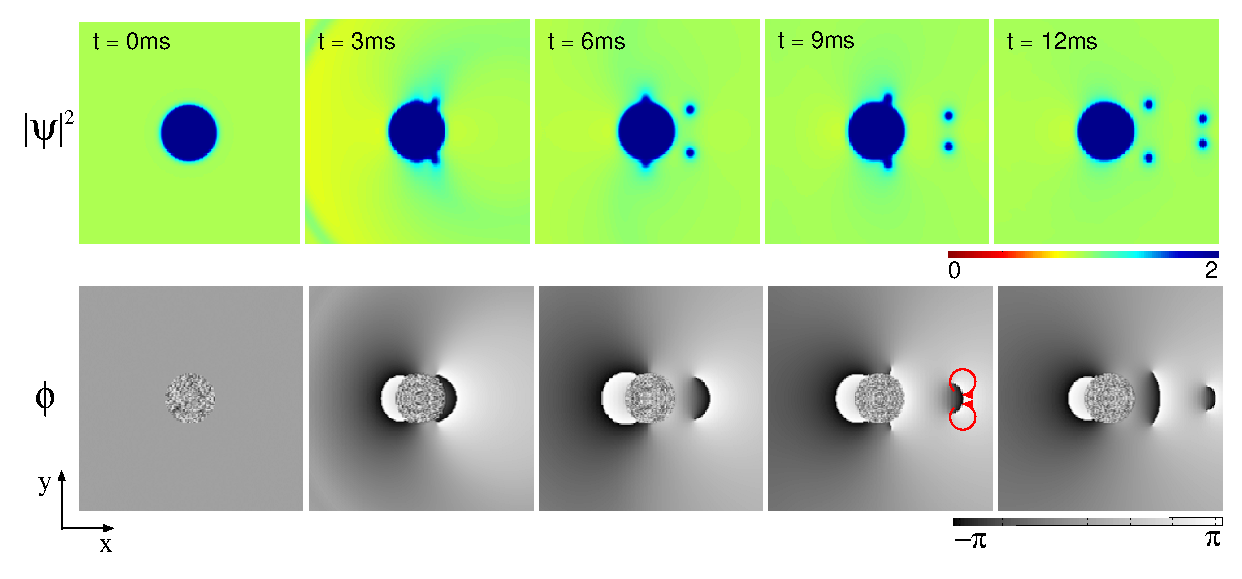
\includegraphics[scale=0.6,keepaspectratio]{3-1.eps}
\caption{
These images shown the dynamics of the vortex shedding in the BEC.
The upper images are the density and the lower images are the phase of the BEC.
The vortices are created behind from the obstacle and rotate in the direction of the red arrows.
}
\label{FIG:3-1}
\end{center}
\end{figure}
Figure 3.1 shows the dynamics of vortex shedding.

\newpage
\section{Results and Discussion}
\subsection{Real Space}
\ We first try to figure out the critical velocity in real space by the Cartesian coordinate.
The critical velocities depend on the diameter of the obstacle.
When the diameter of the obstacle is small, a large velocity is needed to create the vortices.
The healing length $\xi$ and the sound velocity $v_s$ are defined as
$\xi = \frac{1}{\sqrt{4 \pi n_0 a}}\sqrt{1000}$ and $v_s = \frac{\hbar \sqrt{4 \pi n_0 a}}{m}/\sqrt{1000}$.
We numerically obtain the critical velocity.
\begin{figure}[htbp]\begin{center}
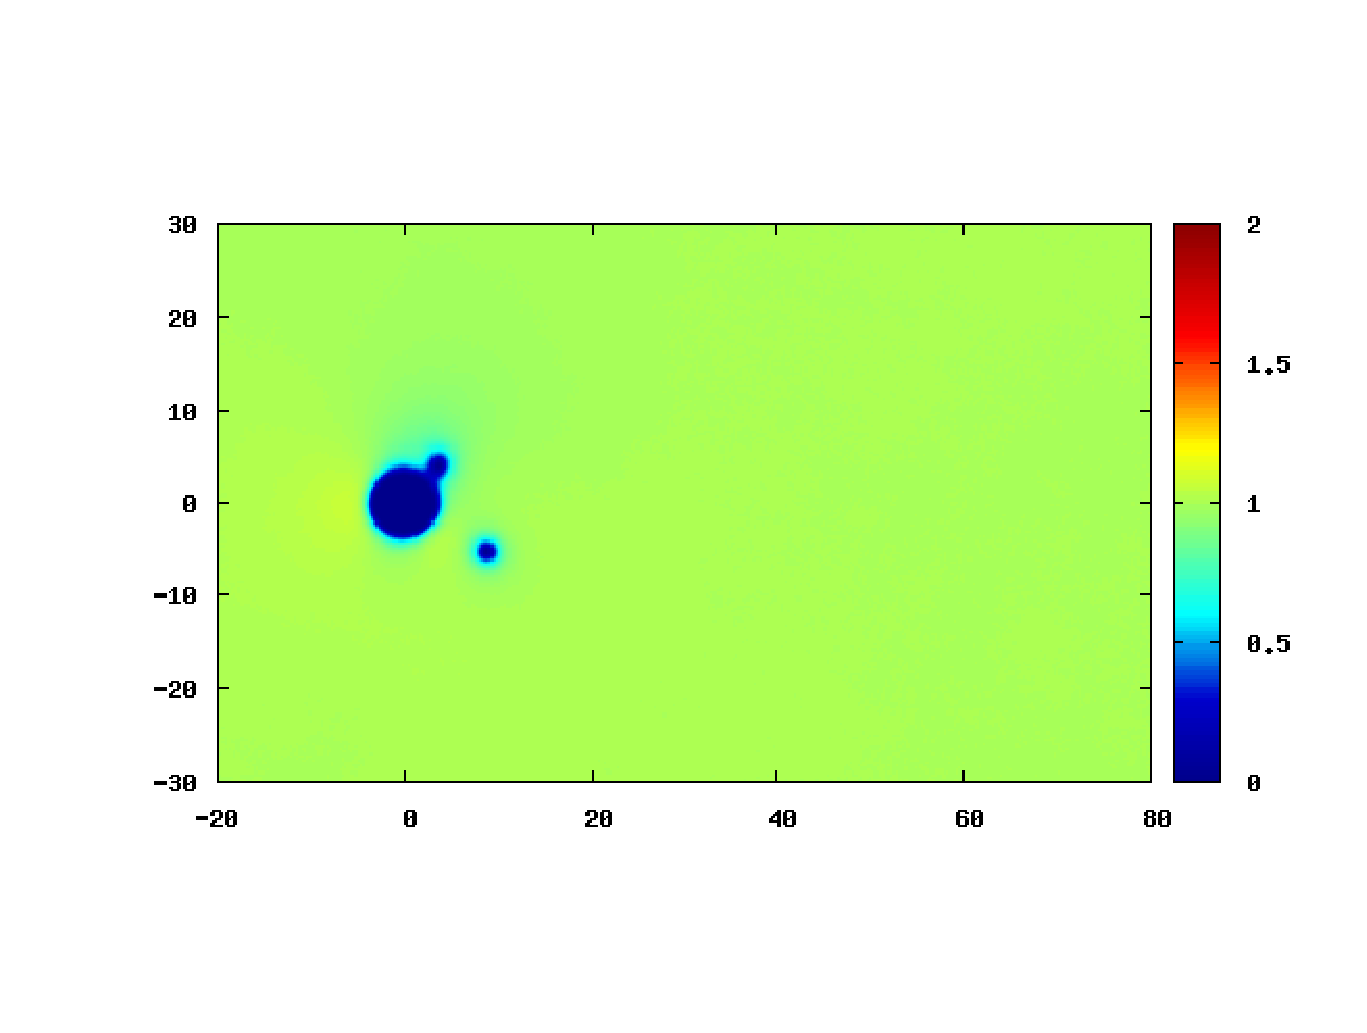
\includegraphics[scale=0.4,keepaspectratio]{3-2.eps}
\caption{
This images shows the density of the BEC.
The vortices start shedding from behind the obstacle which diameter is $6.4\xi$.
}
\label{FIG:3-2}
\end{center}\end{figure}
\\ For example Fig. 3.2 shows the critical velocity is $v_c = 0.4294v_s$ for a diameter $D = 6.4\xi$,
\begin{figure}[htbp]\begin{center}
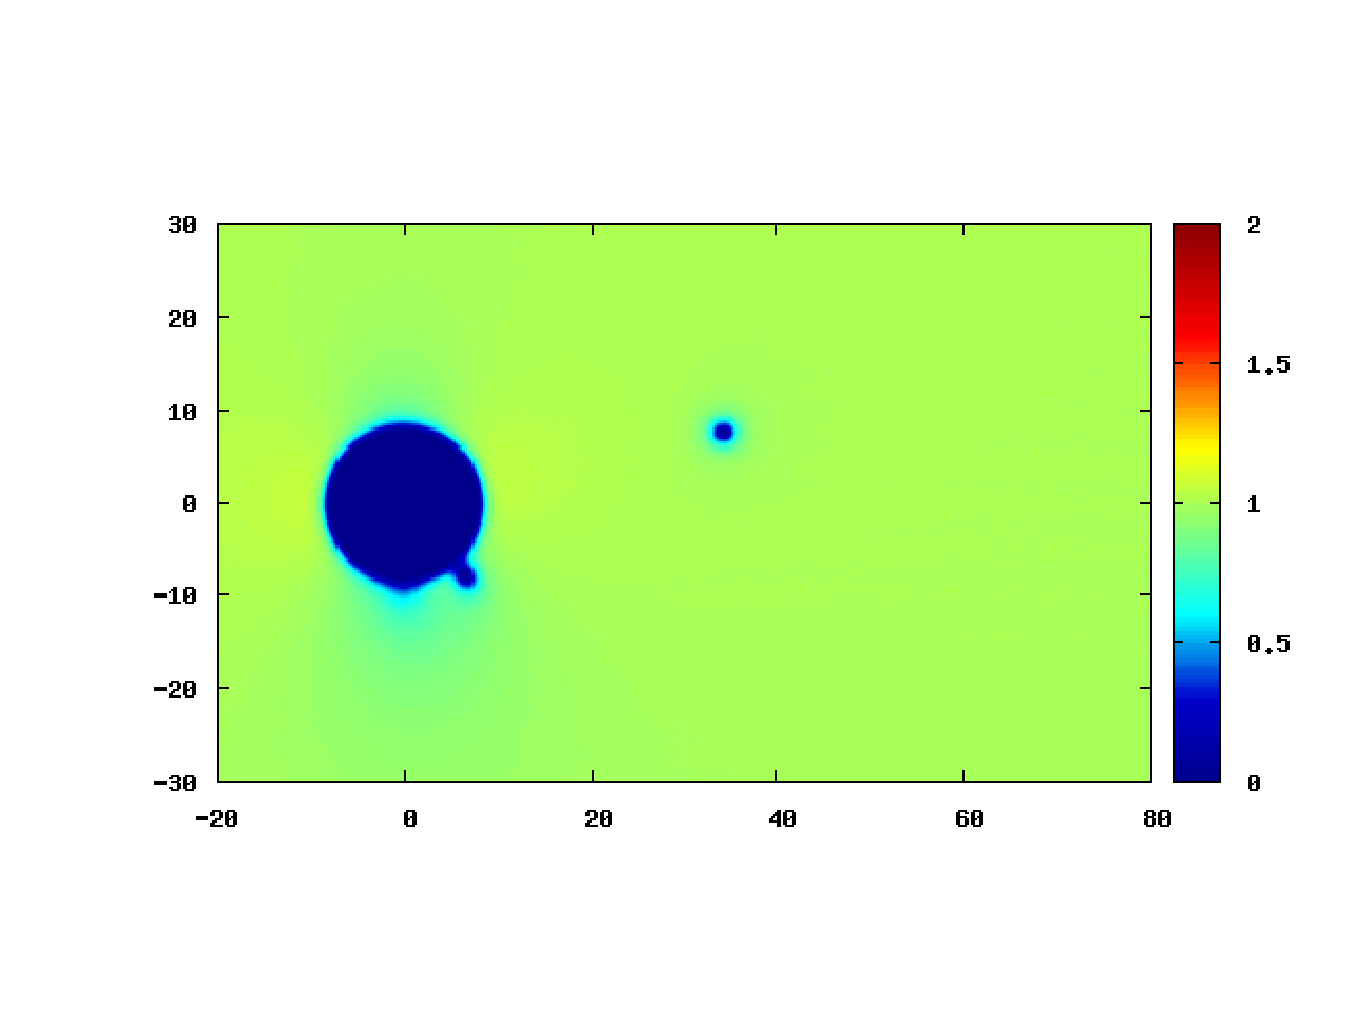
\includegraphics[scale=0.4,keepaspectratio]{3-3.eps}
\caption{
This image shows the density of the BEC.
The vortices start to be created from behind the obstacle whose diameter is $15.8 \xi$.
}
\label{FIG:3-3}
\end{center}\end{figure}
and Fig. 3.3 shows $v_c = 0.401v_s$ for $D = 15.8\xi$.
However, this method is inefficient for systematic investigation of the critical velocity
as a function of the diameter.

\subsection{Initial state}
\ We first prepare the initial state using the imaginary time propagation with some initial velocity.
%\ We noticed that there is a more efficient way.
We try to investigate the critical velocity for the vortex shedding.
We can observe the vortex shedding when the velocity exceeds.
\begin{figure}[htbp]\begin{center}
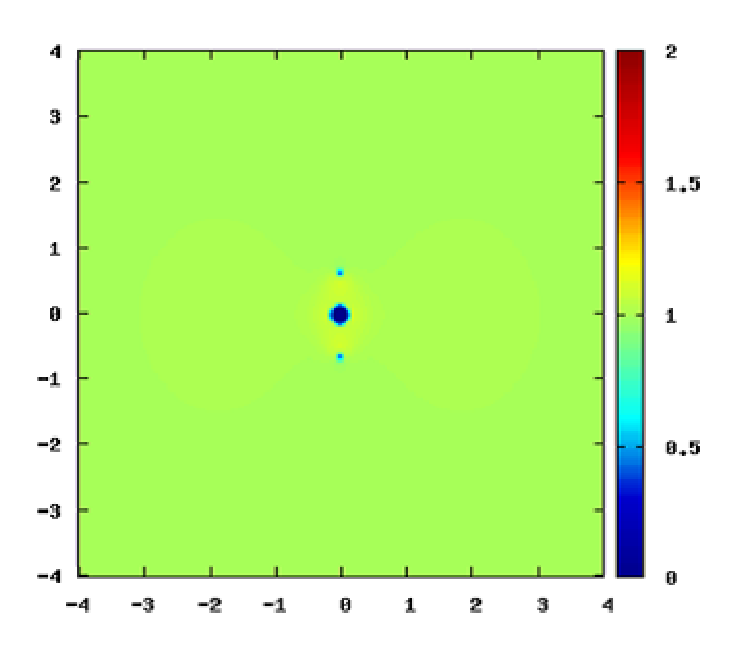
\includegraphics[scale=0.6,keepaspectratio]{3-4.eps}
\caption{
This image shows the density of the BEC at the initial state.
The vortices start to be created from behind the obstacle whose diameter is $0.24\xi$.
}
\label{FIG:3-4}
\end{center}\end{figure}
Figure 3.4 shows the critical velocity is $v_c = 13.9v_s$ for a diameter $D = 0.24\xi$,
\begin{figure}[htbp]\begin{center}
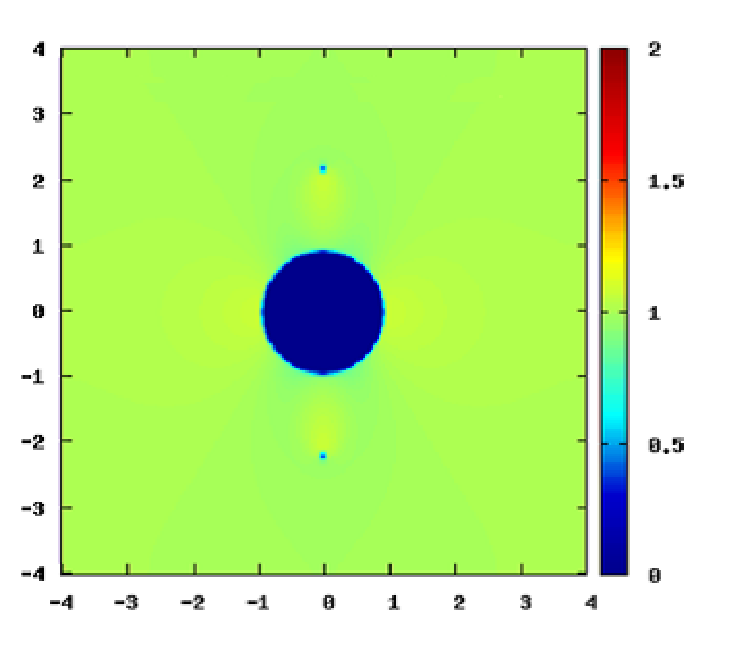
\includegraphics[scale=0.6,keepaspectratio]{3-5.eps}
\caption{
This image shows the density of the BEC at the initial state.
The vortices start to be created from behind the obstacle whose diameter is $2.0\xi$.
}
\label{FIG:3-5}
\end{center}\end{figure}
Figure 3.5 shows $v_c = 0.57v_s$ for $D = 1.9\xi$.

\newpage
\subsection{Polar coordinate system}
\ We next consider the case of a small diameter obstacle.
To assume the high spatial resolution at the edge of the small obstacle wall,
we use the polar coordinate.
\begin{figure}[htbp]\begin{center}
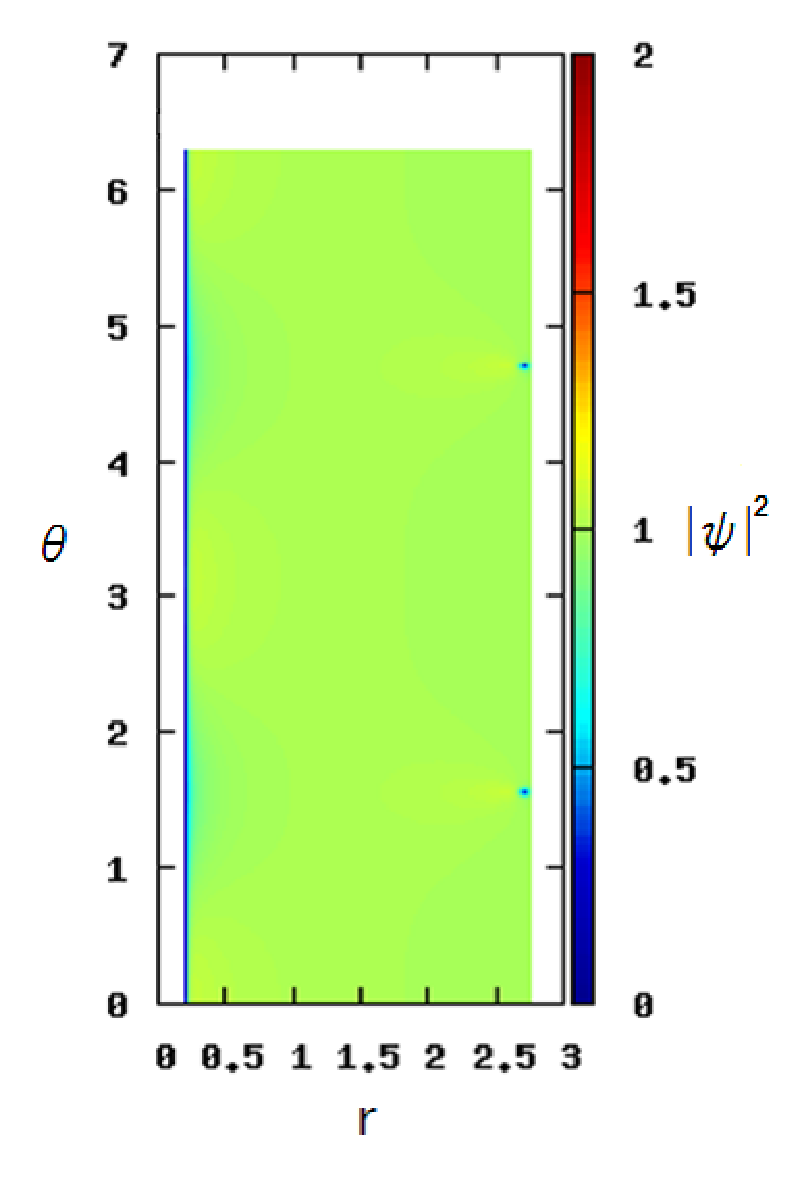
\includegraphics[scale=0.7,keepaspectratio]{3-6.eps}
\caption{
This image shows the density of the BEC with the polar coordinate system.
The vortices start to be created from the side of the obstacle wall whose diameter is $0.1 \xi$
and the critical velocity is larger than $0.5v_s$(Fig.3.6).
}
\label{FIG:3-6}
\end{center}\end{figure}
We can obtain the critical velocity even for a small diameter $D \simeq 0.5 \xi$.
We obtain the critical velocity $v_c = 16.2 v_s$ at the diameter $D = 0.1 \xi$.
\subsection{Limit of $d \rightarrow 0$}
\ We study the $d \rightarrow 0$ limit of the diameter of the obstacle potential.
The wavefunction $\psi$ is very small in the vicinity of the origin.
Then the interaction term is negligible, $g|\psi|^2 = 0$. The Gross-Pitaevskii equation approximated as
\begin{eqnarray}
-\frac{1}{2} \nabla^2 \psi & = & E \psi.
\end{eqnarray}
We use the boundary condition $\psi(r=d)=0$, where the polar coordinate as
\begin{eqnarray}
\frac{\partial^2 \psi}{\partial r^2} + \frac{1}{r}\frac{\partial \psi}{\partial r} + 2E \psi = 0,
\end{eqnarray}
where the interaction energy $E = gn$ and $r = \rho/\sqrt{2E}$.
\\
Hence Eq.(3.10) becomes
\begin{eqnarray}
\frac{\partial^2 \psi}{\partial \rho^2} + \frac{1}{\rho} \frac{\partial \psi}{\partial \rho} + \psi = 0.
\end{eqnarray}
The solution from of Eq.(3.11) is given by the Bessel function as
\begin{eqnarray}
\psi & = & C_1^\prime J_o (\rho) + C_2^\prime Y_o (\rho),
\end{eqnarray}
where $C_1^\prime$ and $C_2^\prime$ are arbitrary constants of integration.
\\
$J, Y$
When the radius take the limit of zero, $\rho \rightarrow 0$,
we use the Bessel functions of the first find.
\begin{eqnarray}
J_o (\rho) & = & 1 + O(\rho^2),
\end{eqnarray}
and use the Bessel functions of the second kind becomes
\begin{eqnarray}
Y_o (\rho) & = & \frac{2}{T_1} \left( \log \frac{\rho}{2} + \gamma \right) J_o (\rho) + O(\rho^2)
\\
& \simeq & \frac{2}{T_1} \left( \log \frac{\rho}{2} + \gamma \right).
\end{eqnarray}
Therefore, we get
\begin{eqnarray}
\psi \simeq C_1 \log \rho + C_2.
\end{eqnarray}
We use the boundary condition as
\begin{eqnarray}
C_1 \log d^\prime + C_2 = 0,
\end{eqnarray}
where $d^\prime = \sqrt{2gn} d$.
We thus obtain
\begin{eqnarray}
\psi \simeq c_1 \log \frac{r}{d}.
\end{eqnarray}
\begin{figure}[htbp]\begin{center}
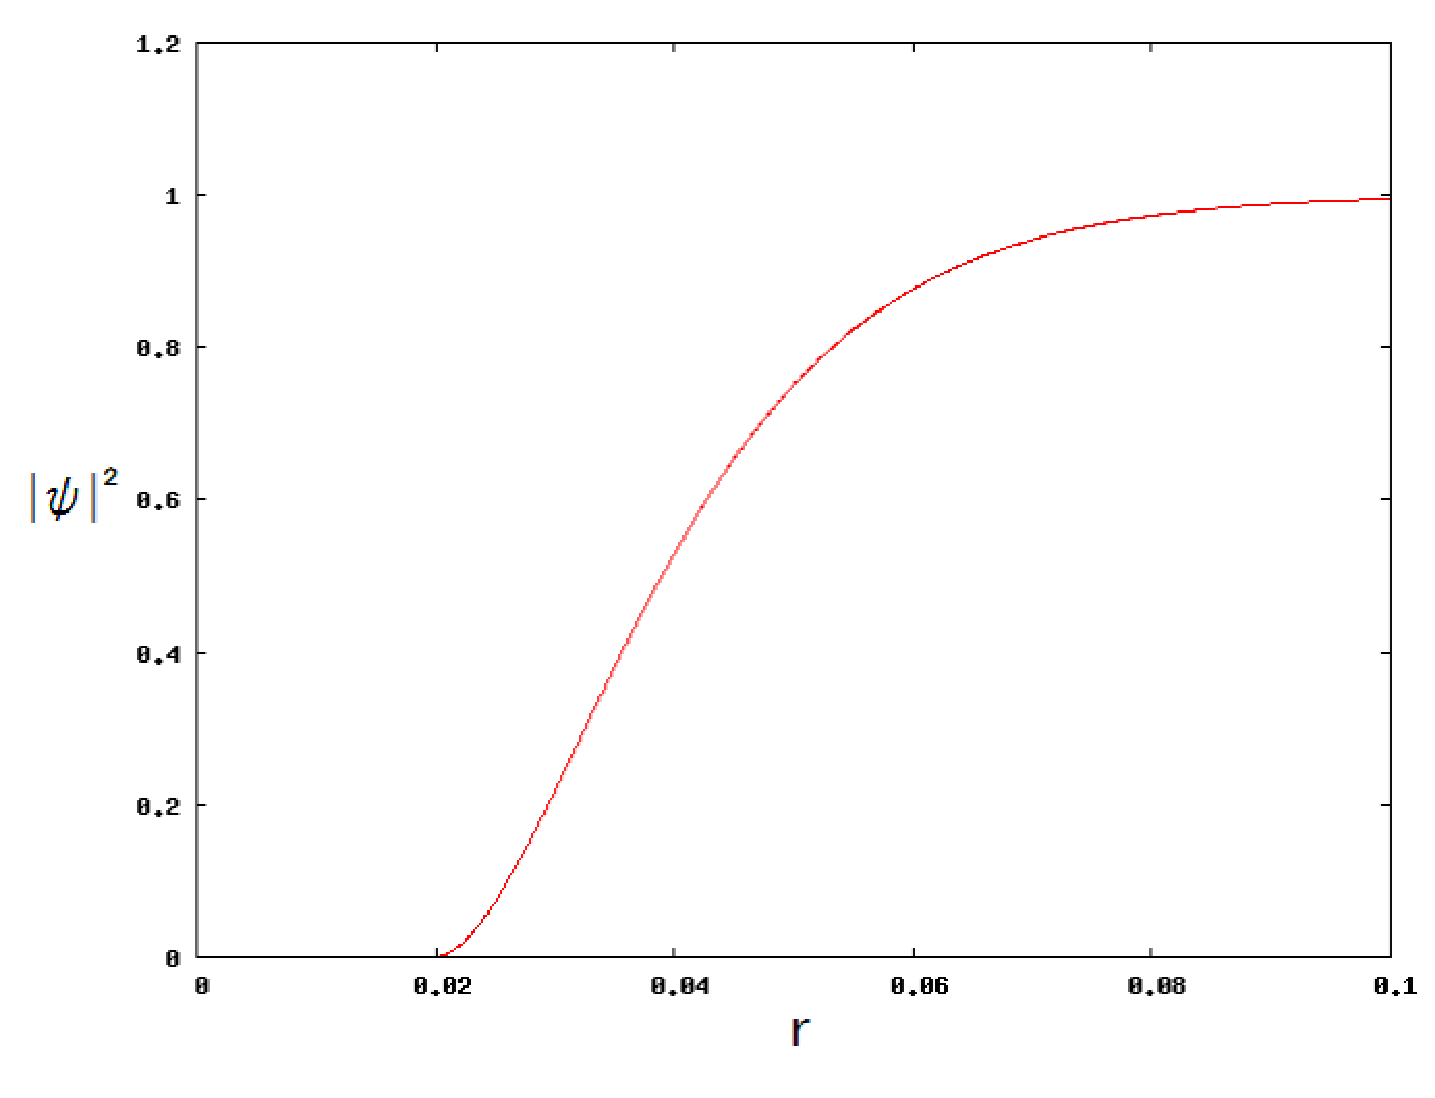
\includegraphics[scale=0.45,keepaspectratio]{3-7.eps}
\caption{
Parameter diagram with respect to the obstacle radius $r$ and the density $|\psi|^2$.
The density curve is downward convex when $r = 0.02 \xi$.
}
\label{FIG:3-7}
\end{center}\end{figure}
\begin{figure}[htbp]\begin{center}
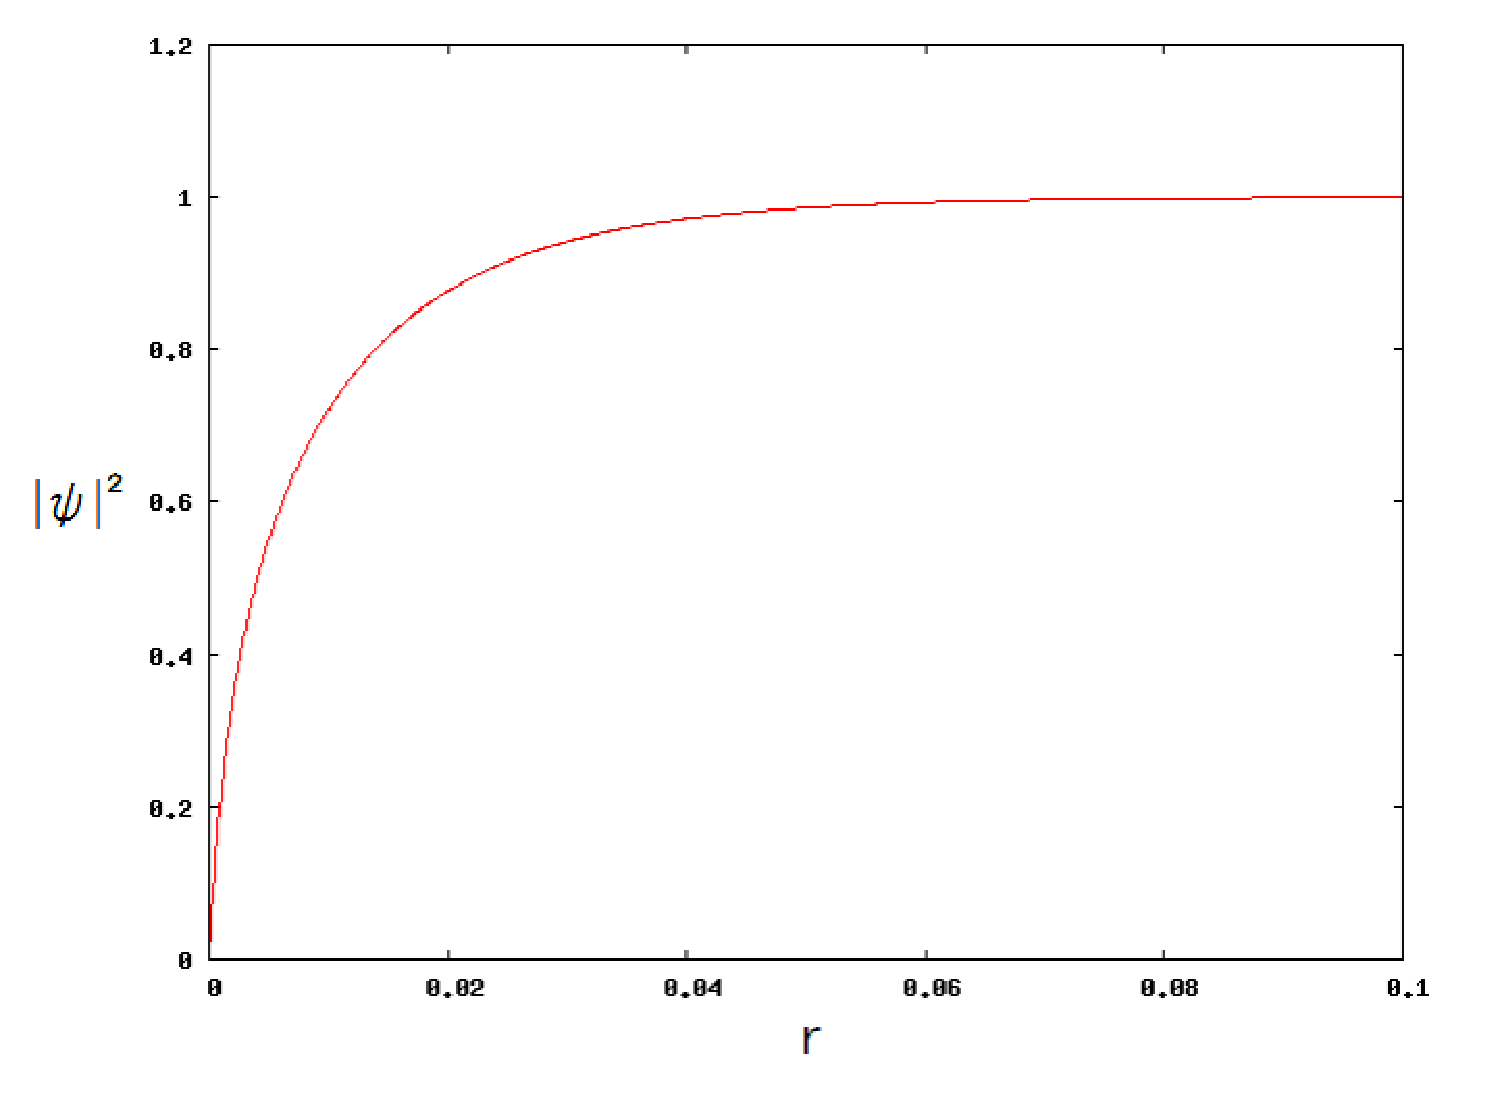
\includegraphics[scale=0.45,keepaspectratio]{3-8.eps}
\caption{
Parameter diagram with respect to the obstacle radius $r$ and the density $|\psi|^2$.
The density curve changes concave whose radius is smaller than $r \simeq 0.0001 \xi$.
}
\label{FIG:3-8}
\end{center}\end{figure}
\ Figures 3.7 and 3.8 shows the density in the vicinity of the center of the potential
for small of decreasing $d$. The curve of the density changes from downward convex (Fig.3.7) to concave (Fig.3.8).
We thus have shown that in the limit of $d \rightarrow 0$,
the wavefunction has the singularity which is physically forbidden.
\newpage
\subsection{Large diameter of the obstacle}
\ We next start, the case of large diameters of the obstacle.
We start from
\begin{eqnarray}
\psi & = & \sqrt{n} e^{i \theta},
\end{eqnarray}
\begin{eqnarray}
i \hbar \frac{\partial \psi}{\partial t} & = &
- \frac{\hbar^2}{2m} \nabla^2 \psi + g | \psi |^2 \psi,
\end{eqnarray}
Substituting Eq.(3.19) into Eq.(3.20), we obtain the real part and the imaginary part as follows
\begin{eqnarray}
\left \{
\begin{array}{l}
\hbar \frac{\partial \sqrt{n}}{\partial t}
= - \frac{\hbar^2}{2m} \left[
2 ( \nabla \theta ) \cdot (\nabla \sqrt{n}) + (\nabla^2 \theta)\sqrt{n}
\right]
\\
-\hbar \sqrt{n} \frac{\partial \theta}{\partial t}
= - \frac{\hbar^2}{2m} \left[
\nabla^2 \sqrt{n} - \sqrt{n} (\nabla \theta)^2
\right]
+ gn \sqrt{n}
\end{array}
\right . ,
\end{eqnarray}
with
\begin{eqnarray}
\vec{v} & = \frac{\hbar}{m} \nabla \theta,
\end{eqnarray}
we have
\begin{eqnarray}
\frac{\partial n}{\partial t} + \nabla \cdot (n \vec{v}) & = & 0.
\end{eqnarray}
This is the equation of continuity for the atoms density.
\\
Equation (3.21) is rewritten as
\begin{eqnarray}
-\frac{\hbar^2}{2m} \frac{1}{\sqrt{n}} + m \frac{\partial}{\partial t} \left( \frac{\hbar}{m} \theta \right)
+ \frac{1}{2} m v^2 + gn & = & 0
\end{eqnarray}
Defining
\begin{eqnarray}
\theta ( \vec{r}, t) & = & \theta( \vec{r} ) - \frac{\mu}{\hbar} t,
\end{eqnarray}
equation (3.24) becomes
\begin{eqnarray}
-\frac{\hbar^2}{2m} \frac{1}{\sqrt{n}} + \frac{1}{2} m v^2 + gn & = & \mu,
\end{eqnarray}
when $n = n_0, v=v_0$, at infinity, we find
\begin{eqnarray}
\frac{1}{2} m v^2(\vec{r}) + gn(\vec{r}) & = & \frac{1}{2} m v_0^2 + gn_0,
\\
n & = & n_0 + \frac{m}{2g} (v_0^2 - v^2 ).
\end{eqnarray}
Substituting Eq.(3.28) into Eq.(3.23), we obtain
\begin{eqnarray}
\nabla \cdot \left[
n_0 \vec{v} + \frac{m}{2g} (v_0^2 - v^2) \vec{v}
\right]
& = & 0.
\end{eqnarray}
Using the sound speed $v_s = \sqrt{\frac{gn_0}{m}}$ and the mach number $M=\frac{v_0}{v_s}$, Eq.(3.29) becomes
\begin{eqnarray}
\nabla \cdot \left \{
\left[
\frac{1}{M^2} + \frac{1}{2}
\left(
1 - \frac{v^2}{v_0^2}
\right) \vec{v}
\right]
\right \} & = & 0,
\end{eqnarray}
using $\vec{v}/v_0 = \nabla \phi$ this expression coincides with Rica's Equation in Ref. \cite[35].
The maximum(critical) velocity is
\begin{eqnarray}
v_{{\rm max}}^2 & = & \frac{gn}{m}
\\
& = & \frac{g}{m} \left[
n_0 + \frac{m}{2g}
\left( v_0^2 - v_{{\rm max}}^2 \right)
\right]
\\
& = & v_s^2 + \frac{1}{2} \left( v_0^2 - v_{{\rm max}}^2 \right).
\end{eqnarray}
Therefore,
\begin{eqnarray}
\frac{1}{M^2} + \frac{1}{2} - \frac{3}{2}\frac{v_{{\rm max}}^2}{v_0^2} & = & 0.
\end{eqnarray}
We try to perform the numerical simulation of the GP equation.
We find that this approach is similar to about same as Rica's paper \cite{35}.

\section{Conclusion}
\begin{figure}[htbp]\begin{center}
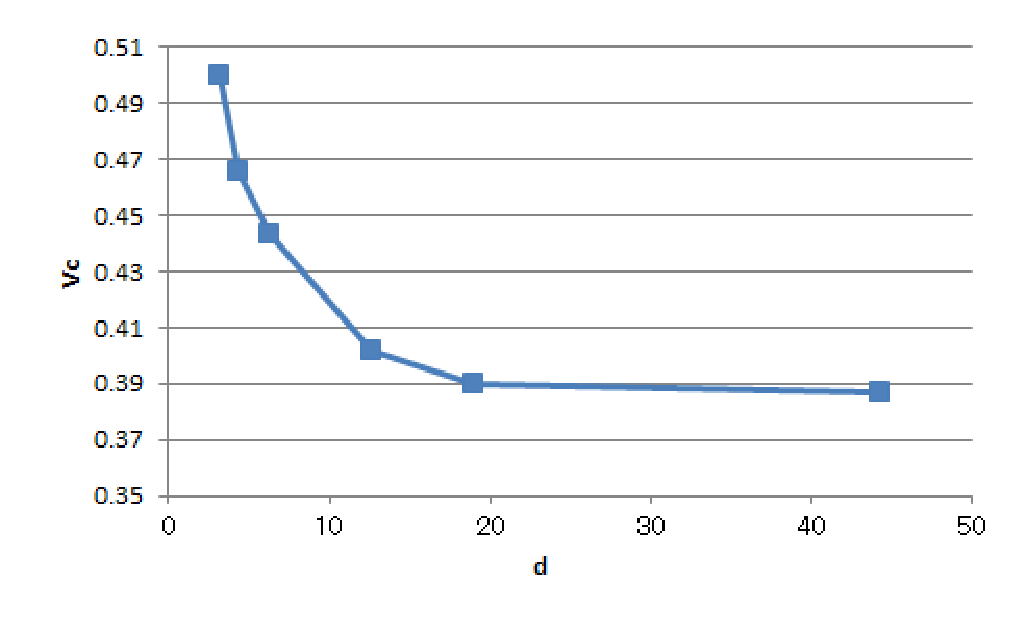
\includegraphics[scale=0.6,keepaspectratio]{3-9.eps}
\caption{
Parameter diagram with respect to the obstacle diameter $d$ and the critical velocity $v_c$.
}
\label{FIG:3-8}
\end{center}\end{figure}
\ Employing the methods we have obtained the critical velocity,
as a function of the size of the potential, We shown in Fig. 3.9.
We compare this result with the previous study
In Ref. \cite{35}, the critical velocity is $v_c \simeq 0.36969(7) v_s$
which agrees with our results.

\chapter{Hysteresis in quantized vortex shedding}
\section{Introduction}
\ The dynamics of fluids can exhibit hysteresis. For example,
a flag-like object shows bistability between flapping and
nonflapping states \cite{36}\cite{37}. Hysteresis also exists
in vortex shedding dynamics behind rigid objects, such
as a vibrating cylinder \cite{38}, a multiple cylinder arrangement \cite{39},
a long cylinder in a three-dimensional flow \cite{40},
and a rod in a soap film \cite{41}. In these experiments, the
transitions between laminar flow and vortex shedding states occur
in a hysteretic manner as a function of the Reynolds number.
It is known that the Taylor-Couette flow also exhibits hysteresis \cite{42}.
In superfluids, hysteresis has been observed in rotating toroidal system \cite{43} \cite{44}.
\ We consider transition between a laminar
flow state and a quantized vortex-shedding state around
an obstacle moving in a BEC. In a superfluid,
the velocity field around an obstacle is irrotational
below the critical velocity.When the velocity of the obstacle
exceeds the critical velocity, quantized vortices are
created and released behind the obstacle, as observed in a trapped BEC
stirred by an optical potential \cite{30} \cite{45} \cite{46}. The critical velocity
for vortex creation and the dynamics of quantized vortex
shedding in superfluids have been studied theoretically by many researchers \cite{19}\cite{21}\cite{22}\cite{24}\cite{31}\cite{33}\cite{35}\cite{47}\cite{48}\cite{49}\cite{50}\cite{51}\cite{52}\cite{53}\cite{54}.
\\
\ The purpose of this study is to show that superfluids
undergo hysteric changes between stationary laminar flow
and periodic shedding of quantized vortices. Consider an
obstacle with gradually increasing velocity; on reaching the
critical velocity $V_{c1}$, periodic vortex shedding starts. Now
consider an obstacle with gradually decreasing velocity from
above $V_{c1}$; the vortex shedding stops at a velocity $V_{c2}$. We
show that there is a bi-stability between these flow patterns,
i.e., $V_{c2} < V_{c1}$. Although hysteric vortex shedding under a
moving potential was reported by the authors of Ref.\cite{33},
the mechanism has not been studied in detail.
We show that the hysteric behaviors are due to the
fact that released vortices enhance the flow velocity around
the obstacle and induce subsequent vortex creation. We show
that the hysteric behavior is observed for a circular obstacle
moving in a two-dimensional (2D) superfluid and a spherical
obstacle moving in a three-dimensional (3D) superfluid.
%\ We get the critical velocities of the vortex shedding in a constant velocity field.
%A@AXChA
%Qx炸A
%炭gOAQ
%B
%Although the vortex shedding is stop because of under the critical velocity.
%And after a while, a phenomena appears that the vortex continue regenerate with a trigger
%anything disturbance.
%AxCx(Vc2)A
%xグCx(Vc1)
%qXeVXJA
%oB
%We assume that the system has the hysteresis interval as the bi-stability
%which contains the critical velocity of the accelerate direction(Vc1) and
%the decelerate direction(Vc2).
%ExB
%fast of all, the critical velocity in the quasi-static deceleration
%xxQB
%the vortex shedding will be stop
%|eVa12.6AQEx0.39B
%in the case of the radius scale equal to $12.6\xi$, the critical velocity for ing the vortex shedding is
%$0.39 v$
%a12.6AxグQx0.42
%Ex0.41B
%炫0.02AoB
%x|eVaQo邱B
%We found out a bi-stability in quantized vortex shedding under a conditions of velocity and potential size.
%(fig1`4)
%@oAQxAQxx
%AIB|eVaQomFB
%QxA|eVUh
%Q邱omFB
%@AJ}Qx|eVao
%mF邱B
%{nBECzqQsB
%@ABECfGross-Pitaevskii
%lvZpQl@B
%O|eV~`|eVfOA
%|eVaRAxvAp[^ωB
%BAQxExB
%A|eVlKEVA
%ωe}B
%|eV邪A
%Qlq~
%|eVΑx[A
%|eVJ@B
%Af~APVsAPB
%@lvZpA
%|eVaExOtB
%|eVaAcx\B
%|eVaExlA0.4A
%s_l(0.36969(7))B
%AaExlA
%0.5tB
%AQx炸A
%炭gOA
%QB
%|eVa2.53AEx0.42
%rQAlqB
%AxCx(Vc2)A
%xグCx(Vc1)
%qXeVXJA
%oB
%Ex
%|eVa12.6A
%QEx(Vc2)0.39B
%rQlq
%B
%First the critical velocity of the deceleration,
%The vortex shedding is stop in the case of the potential diameter is 12.6.
%Aa12.6AxグA
%rQB
%Ex(Vc1)0.41B
%炫0.02A
%o
%There is the property of the bi-stability.
%OtAoAcxxA
%a4.1lq\B
%x0.43QAExA
%|eVuA|eV^A
%gK[QB
%AQtA
%|eVuA
%uB
%the blue circle the red circle
%xs[NAQlqB
%Qxs[N
%x邱B
%The vortex is created when the local velocity is the peak.
%AoQyAAQ|eVz
%_QnSAkfpB
%
%}fOtB
%QuWB
%
%AQQvA
%aR|eVvQB
%AzaA|eVOuA
%ASl邨Q{x
%AQB
%AxオA|eV
%QlB
%AIQyAo
%ExVc1A
%|eVNxω
%JQAqXeVX邱B
%OtB
%QAQ
%o邱B
%Vc1|eVExA
%Vc2ExAoJB
%|eVao悪A
%QExオ邱B
%OlqmFB
%Next, we also investigate the situation of the three-dimensional system.
%x\AKEVA|eVpB
%A6.3aB
%XChAX0.6VsxJnA
%lqr|eV^A
%QgK[B
%ExA0.595VsQB
%A0.601VsQonAExJA0.06VsA
%OoB
%AQAQyAOQ邱CtB
%We notice the vortex and anti-vortex pair in 2 dimensions are
%applied to the vortex ring in 3 dimensions.
%AQ]A
%OB
%AQQB
%%AOAwI炸A
%o[vB
%It is interesting both of these systems include bi-stability although .
%Thus, although the feature differ in topology by two dimension and three dimension systems,
%it is considered to be interesting to have both o.  suitability.
%AB
%BECA
%|eVaAxQqXeVXB
%AnAOno悪邱B
%W]Agbv|eVno
%邱vB
\section{Formulation of the problem}
\ We study the dynamics of a BEC at zero temperature
using mean-field theory. The system is described by the
Gross-Pitaevskii (GP) equation
\begin{eqnarray}
i \hbar \frac{\partial \Psi}{\partial t} & = &
- \frac{\hbar^2}{2m} \nabla^2 \Psi + U(\vec{r},t)\psi + \frac{4 \pi^2 a}{m} | \Psi |^2 \psi.
\end{eqnarray}
where $\Psi(\vec{r},t)$ is the macroscopic wave function, $m$ is the
atomic mass, $U( \vec{r}, t)$ is an external potential,and a is
the $s$-wave scattering length. We consider situations in
which a localized potential $u$ moves at a velocity $\vec{V}(t)$,
i.e., the potential $U$ has a form,
\begin{eqnarray}
U(\vec{r},t) & = & u \left( \vec{r} - \int_0^t \vec{V}(t^\prime) \diff t^\prime, t \right).
\end{eqnarray}
We transform Eq.(4.1)into the frame of reference of the
moving potential $U$ by substituting the unitary transformation.
\begin{eqnarray}
\Psi \left( \vec{r}, t \right) & = & \exp \left[ - \int^t \vec{V} \left( t^\prime \right) \diff t^\prime \cdot \nabla \right]
\psi \left( \vec{r}, t \right)
\end{eqnarray}
into Eq.(4.1), which yields
\begin{eqnarray}
i \hbar \frac{\partial \psi}{\partial t} & = &
- \frac{\hbar^2}{2m} \nabla^2 \psi + i \hbar \vec{V} \cdot \nabla \psi
+ u \left( \vec{r}, t \right) + \frac{4 \pi \hbar^2 a}{m} | \psi |^2 \psi .
\end{eqnarray}
In the following, the velocity vector is taken as
\begin{eqnarray}
\vec{V} (t) & = & - V(t) \hat{x}.
\end{eqnarray}
where $\hat{x}$ is the unit vector in the x direction.
\\
\ We consider an infinite system, in which the atomic
density $| \psi |^2$ far from the moving potential is
constant $n_0$. For the density $n_0$, the healing length
$\xi$ and the sound velocity $v_s$ are defined as
\begin{eqnarray}
\xi \equiv \frac{1}{\sqrt{4 \pi n_0 a}}, \ \ v_s \equiv \frac{\hbar \sqrt{4 \pi n_0 a}}{m},
\end{eqnarray}
which determine the characteristic time scale,
\begin{eqnarray}
\tau & = & \frac{\xi}{v_s}.
\end{eqnarray}
The chemical potential for the density $n_0$ is given by
\begin{eqnarray}
\mu & = & \frac{4 \pi \hbar^2 a}{m} n_0.
\end{eqnarray}
Normalizing Eq.(4.4) by the quantities in Eqs.(4.6)-(4.8), we obtain
\begin{eqnarray}
i \frac{\partial \tilde{\psi}}{\partial \tilde{t}} & = &
- \frac{1}{2} \tilde{\nabla^2} \tilde{\psi}
+ i \tilde{\vec{V}} \tilde{\psi}
+ \tilde{u} \tilde{\psi}
+ | \tilde{\psi} |^2 \tilde{\psi},
\end{eqnarray}
where $\tilde{\psi} = n_0^{-1/2}, \tilde{t} = t/\tau, \tilde{\nabla} = \xi \nabla, \tilde{\vec{V}} = \vec{V}/v_s,$
and $\tilde{u} = u/\mu$ are dimensionless quantities. The independent
parameters in Eq.(4.9) are only $\tilde{\vec{V}}$ and $\tilde{u}$.
\\
\ We numerically solve Eq.(4.9) using the pseudo-spectral method \cite{34}.
The initial state is a stationary state of Eq.(4.9) for a velocity $V$ below the critical velocity $V_{c1}$ for
vortex nucleation,
which is prepared by the imaginary-time propagation method \cite{55}.
The initial state is a stationary laminar flow and contains no vortices.
To break the exact numerical symmetry,
a small random noise is of magnitude $\sim 10^{-3} \sqrt{n_0}$ is
added to each mesh of the initial state.
The results are qualitatively insensitive to the magnitude of the noise.
The real-time propagation of Eq.(4.9) is
then calculated with a change in the velocity $V$
or the potential $u$ to trigger the
vortex creation.
The size of the space is taken to be large
enough and the periodic boundary condition imposed by
the pseudo-spectral method does not affect the dynamics
around the potential.
\section{Results and Discussion}
\subsection{Two dimensional system}
\ First, we consider a 2D space. Typically, the size of
the numerical space is taken to be $512 \xi$ in $x$ and $256 \xi$ in
$y$, and is divided into a $8192 \times 4096$ mesh. The obstacle
potential is given by
\begin{eqnarray}
u \left( \vec{r} \right) & = &
\left \{
\begin{array}{l l}
\infty & ( \sqrt{x^2+y^2} < R ),
\\
     0 & ( \sqrt{x^2+y^2} > R ),
\end{array}
\right.
\end{eqnarray}
where $R$ is the radius of the circular potential.
Numerically, a value that is significantly larger than the chemical
potential is used for $\infty$ in Eq.(4.10). The following results
are qualitatively the same as those for a Gaussian potential in place
of the rigid circular potential in Eq.(4.10).
\\
\begin{figure}[htbp]
\begin{center}
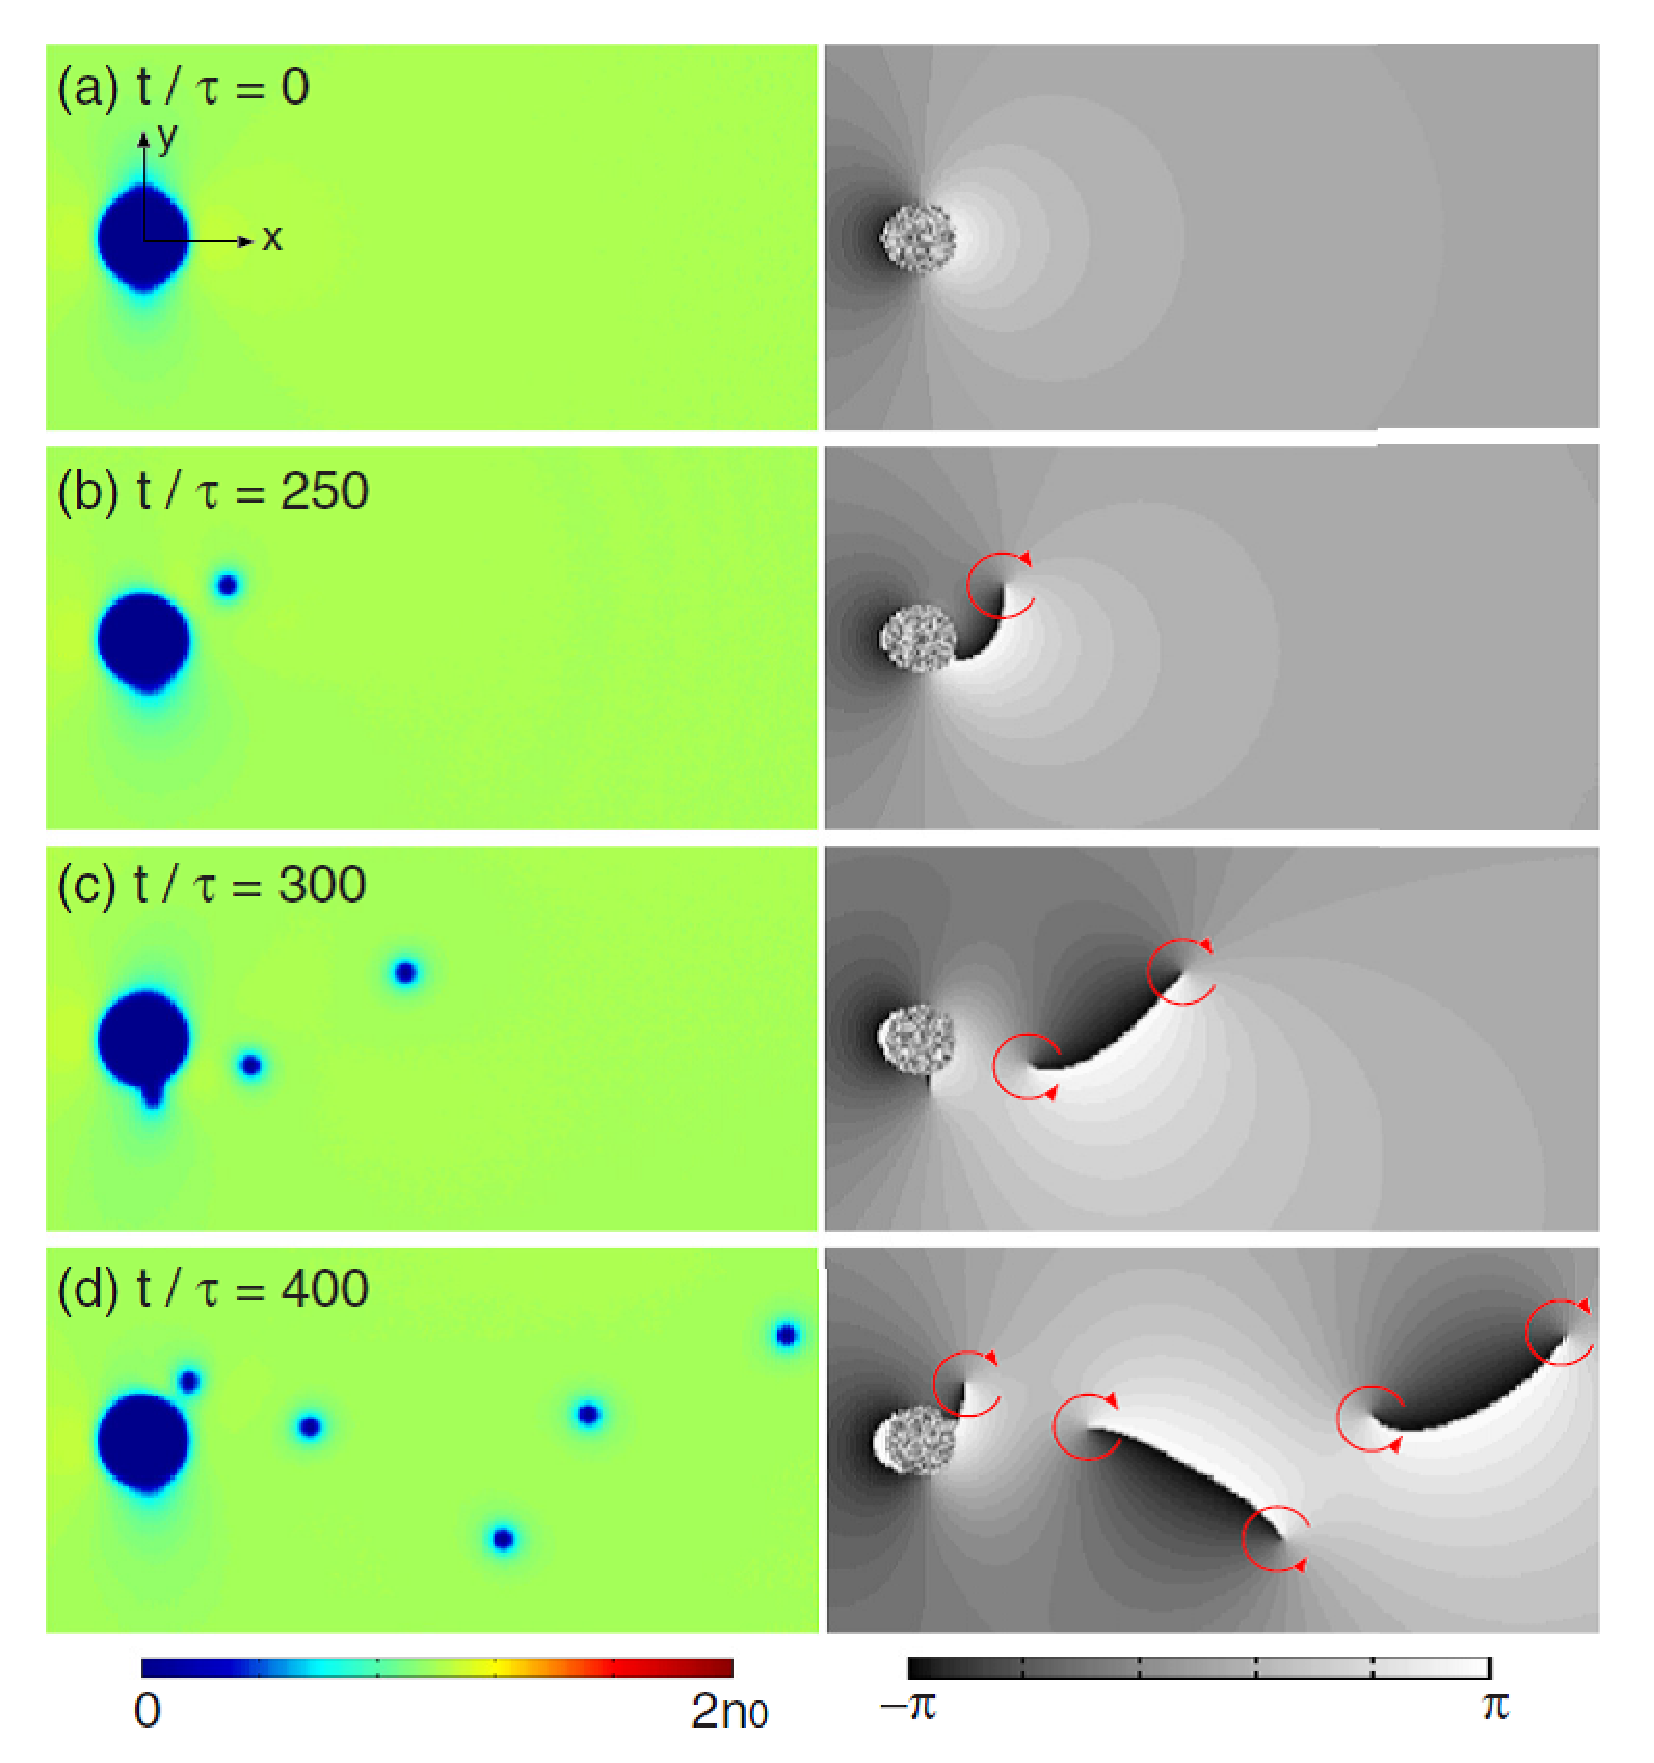
\includegraphics[scale=0.40, keepaspectratio]{4-1.eps}
\caption{
Time evolution of the density $|\psi|^2$(left
panels) and phase arg$\psi$ (right panels) profiles for $V = 0.43 v_s$ and
$R=4.1 \xi$. To trigger the vortex shedding, the additional potential
given by Eq. (4.11) is applied during $200 < t/\tau < 220$. The arrows
in the phase profiles indicate the directions in which the quantized
vortices are rotating. The size of each panel is $80 \xi \times 40 \xi$ .
}
\label{FIG:4-1}
\end{center}
\end{figure}
\ Figure 4.1 shows the time evolution of the density $|\psi|^2$
and phase arg $\psi$ profiles. The initial state is the stationary
state for the velocity $v=0.43 v_s$ and radius $R=4.1 \xi,$
as shown in Fig. 4.1(a). This stationary laminar flow state
in stable. To trigger the vortex shedding, we apply an
additional potential,
\begin{eqnarray}
u_{{\rm add}} \left( \vec{r} \right) & = &
\mu e^{- \left[ x^2 + \left( y - R\right)^2 \right] / \xi^2}
\end{eqnarray}
during $200 < t/\tau < 220$, in addition to the circular
potential in Eq.(4.10). This additional potential perturbs the
edge of the circular potential, at which quantized vortex
creation is induced, as shown in Fig. 4.1(b). Subsequently,
quantized vortices are periodically created one after the other \cite{52}.
as shown in Fig. 4.1(c) and Fig. 4.1(d), even after the
perturbation potential is removed at $t=220 \tau$ and the
velocity $v= 0.43 v_s$ is smaller than the critical velocity
$V_{c1}$. This result indicates that there are at least
two stable flow patterns for the same parameters: a stationary
laminar flow and periodic vortex shedding.
\\
\ The velocity field of the atomic flow has the form,
\begin{eqnarray}
\vec{v} \left( \vec{r}, t \right) & = &
\frac{\hbar}{2 m i | \psi |^2} \left( \psi \nabla \psi^* - \psi^* \nabla \psi \right) - \vec{V}.
\end{eqnarray}
\begin{figure}[htbp]
\begin{center}
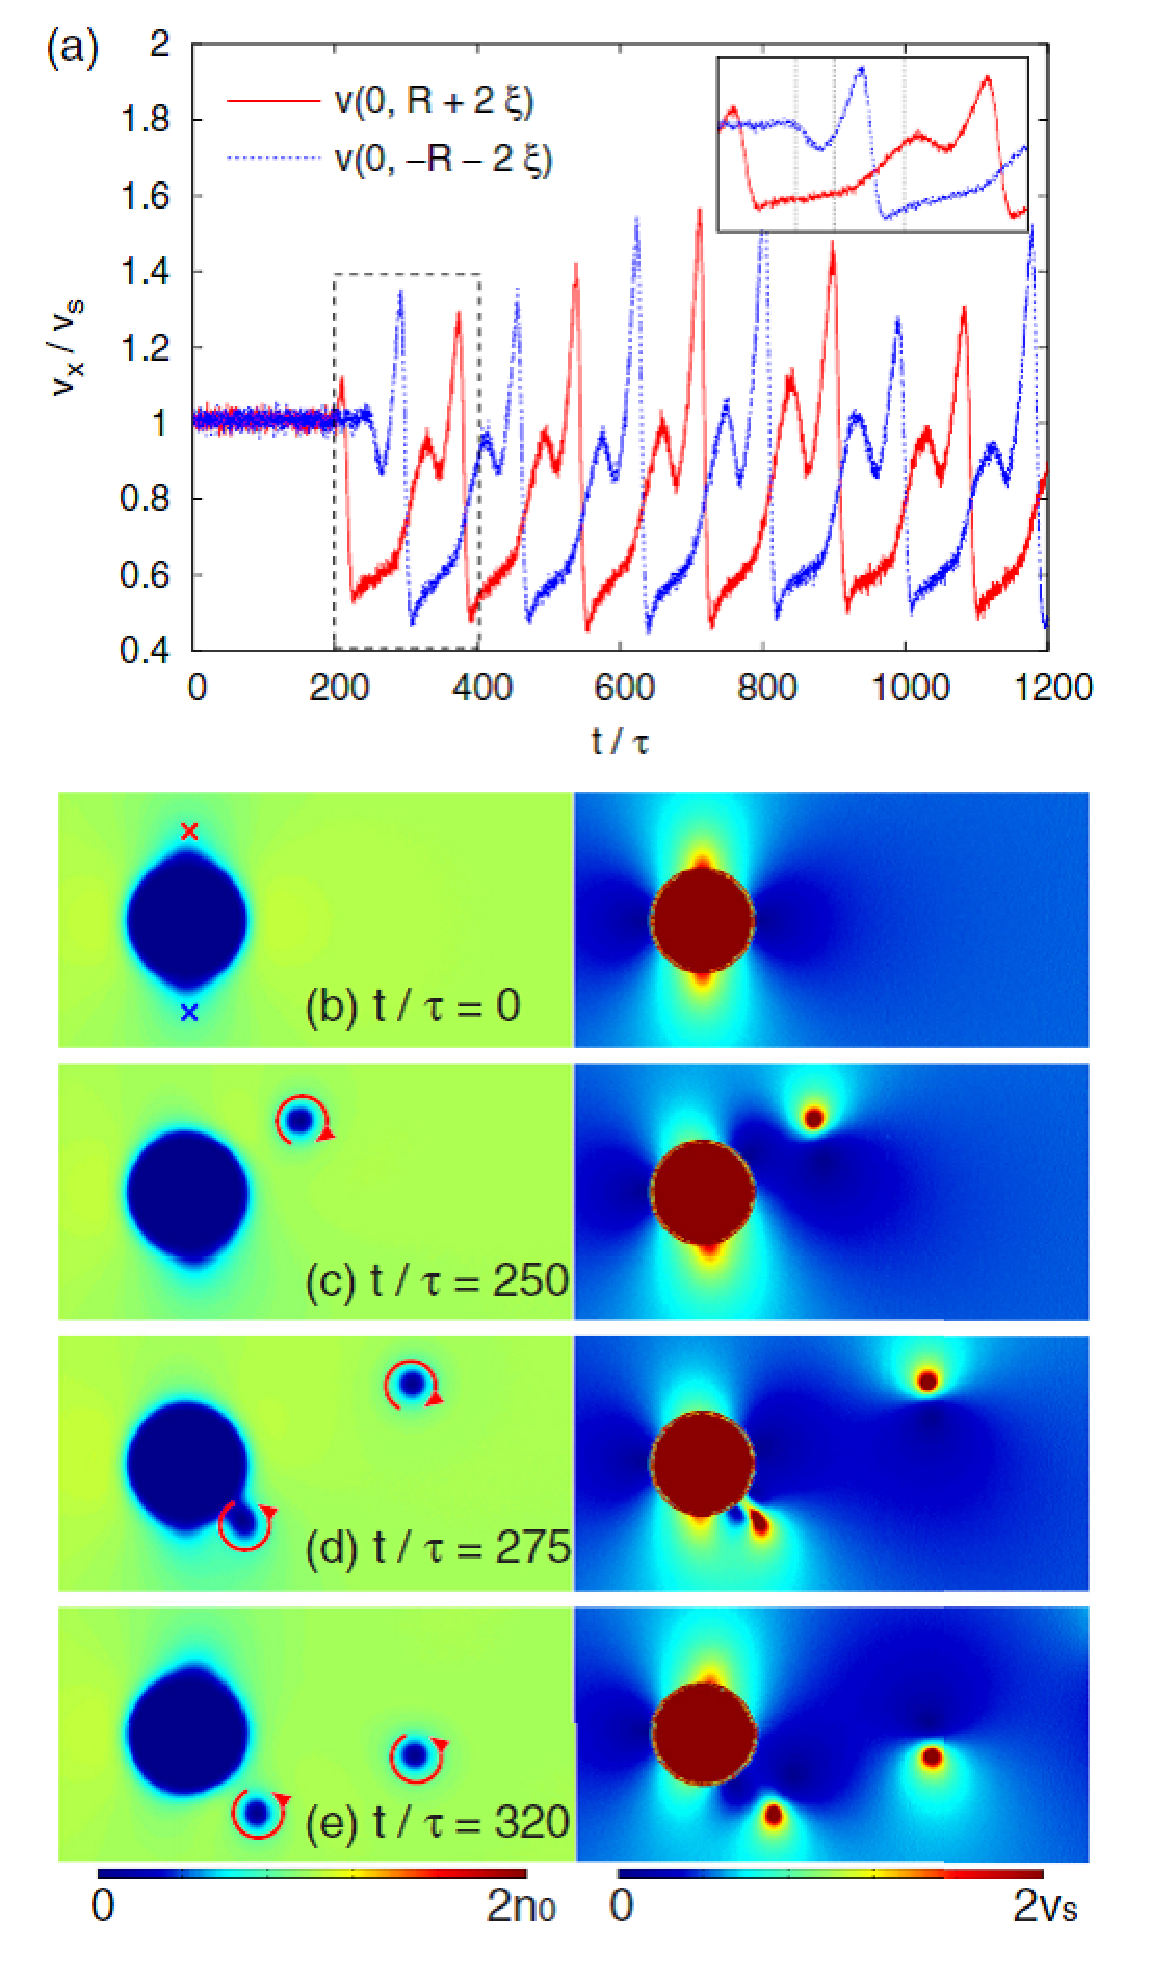
\includegraphics[scale=0.53, keepaspectratio]{4-2.eps}
\caption{
(a) Time evolution of the velocity $v_x$ at
$(x,y)=(0, \pm R \pm 2 \xi$ for the same parameters as those in Fig. 4.1.
The dashed square is magnified in the inset, where the vertical lines
indicate $t/\tau = 250,275,$ and $320$. (b)-(e) Density $|\psi|^2$ profiles (left
panels) and velocity $|v|$ profiles (right panels). The crosses in (b)
indicate the positions $(x,|y|)=(0,R+2 \xi)$ at which the velocities
are plotted in (a). The arrows in the density profiles indicate the
directions in which the quantized vortices are rotating. The size of
each panel is $40 \xi \times 20 \xi$.
}
\label{FIG:4-2}
\end{center}
\end{figure}
\ Figure 4.2(a) shows the time evolution of the velocities
$v_x$ at $ \left( x, |y| \right) = \left( 0, R + 2 \xi \right)$.
These positions are indicated by the crosses in Fig. 4.2(b).
For the stationary flow $(t < 200 \tau),$ the velocities are
$v_x \simeq v_s$. The fluctuations around $v_s$ are due to
the small numerical noises added
to the initial state. At $t=200 \tau$, the additional potential
given by Eq.(4.11) is applied and a clockwise vortex is
released from near the position $\left( 0, R \right)$. As a consequence,
$v_x \left( 0, R+ 2 \xi \right)$ suddenly decreases. It can also be seen in
Fig. 4.2(c) that the released vortex decreases the velocity
field in the vicinity of its creation. The clockwise vortex
shedding then induces counter-clockwise vortex creation,
as shown in Fig. 4.2(d). Immediately after that $(t=275 \tau -320 \tau),
v_x(0,-R-2\xi)$ increase rapidly, which is followed
by a sudden decrease due to the shedding of another
counter-clockwise vortex, as shown in Fig. 4.2(d). This
dynamics shown in Fig. 4.2 implies that the release of a
vortex induces the creation of a subsequent vortex, i.e.,
periodic vortex shedding is taking place.
\\
\begin{figure}[htbp]
\begin{center}
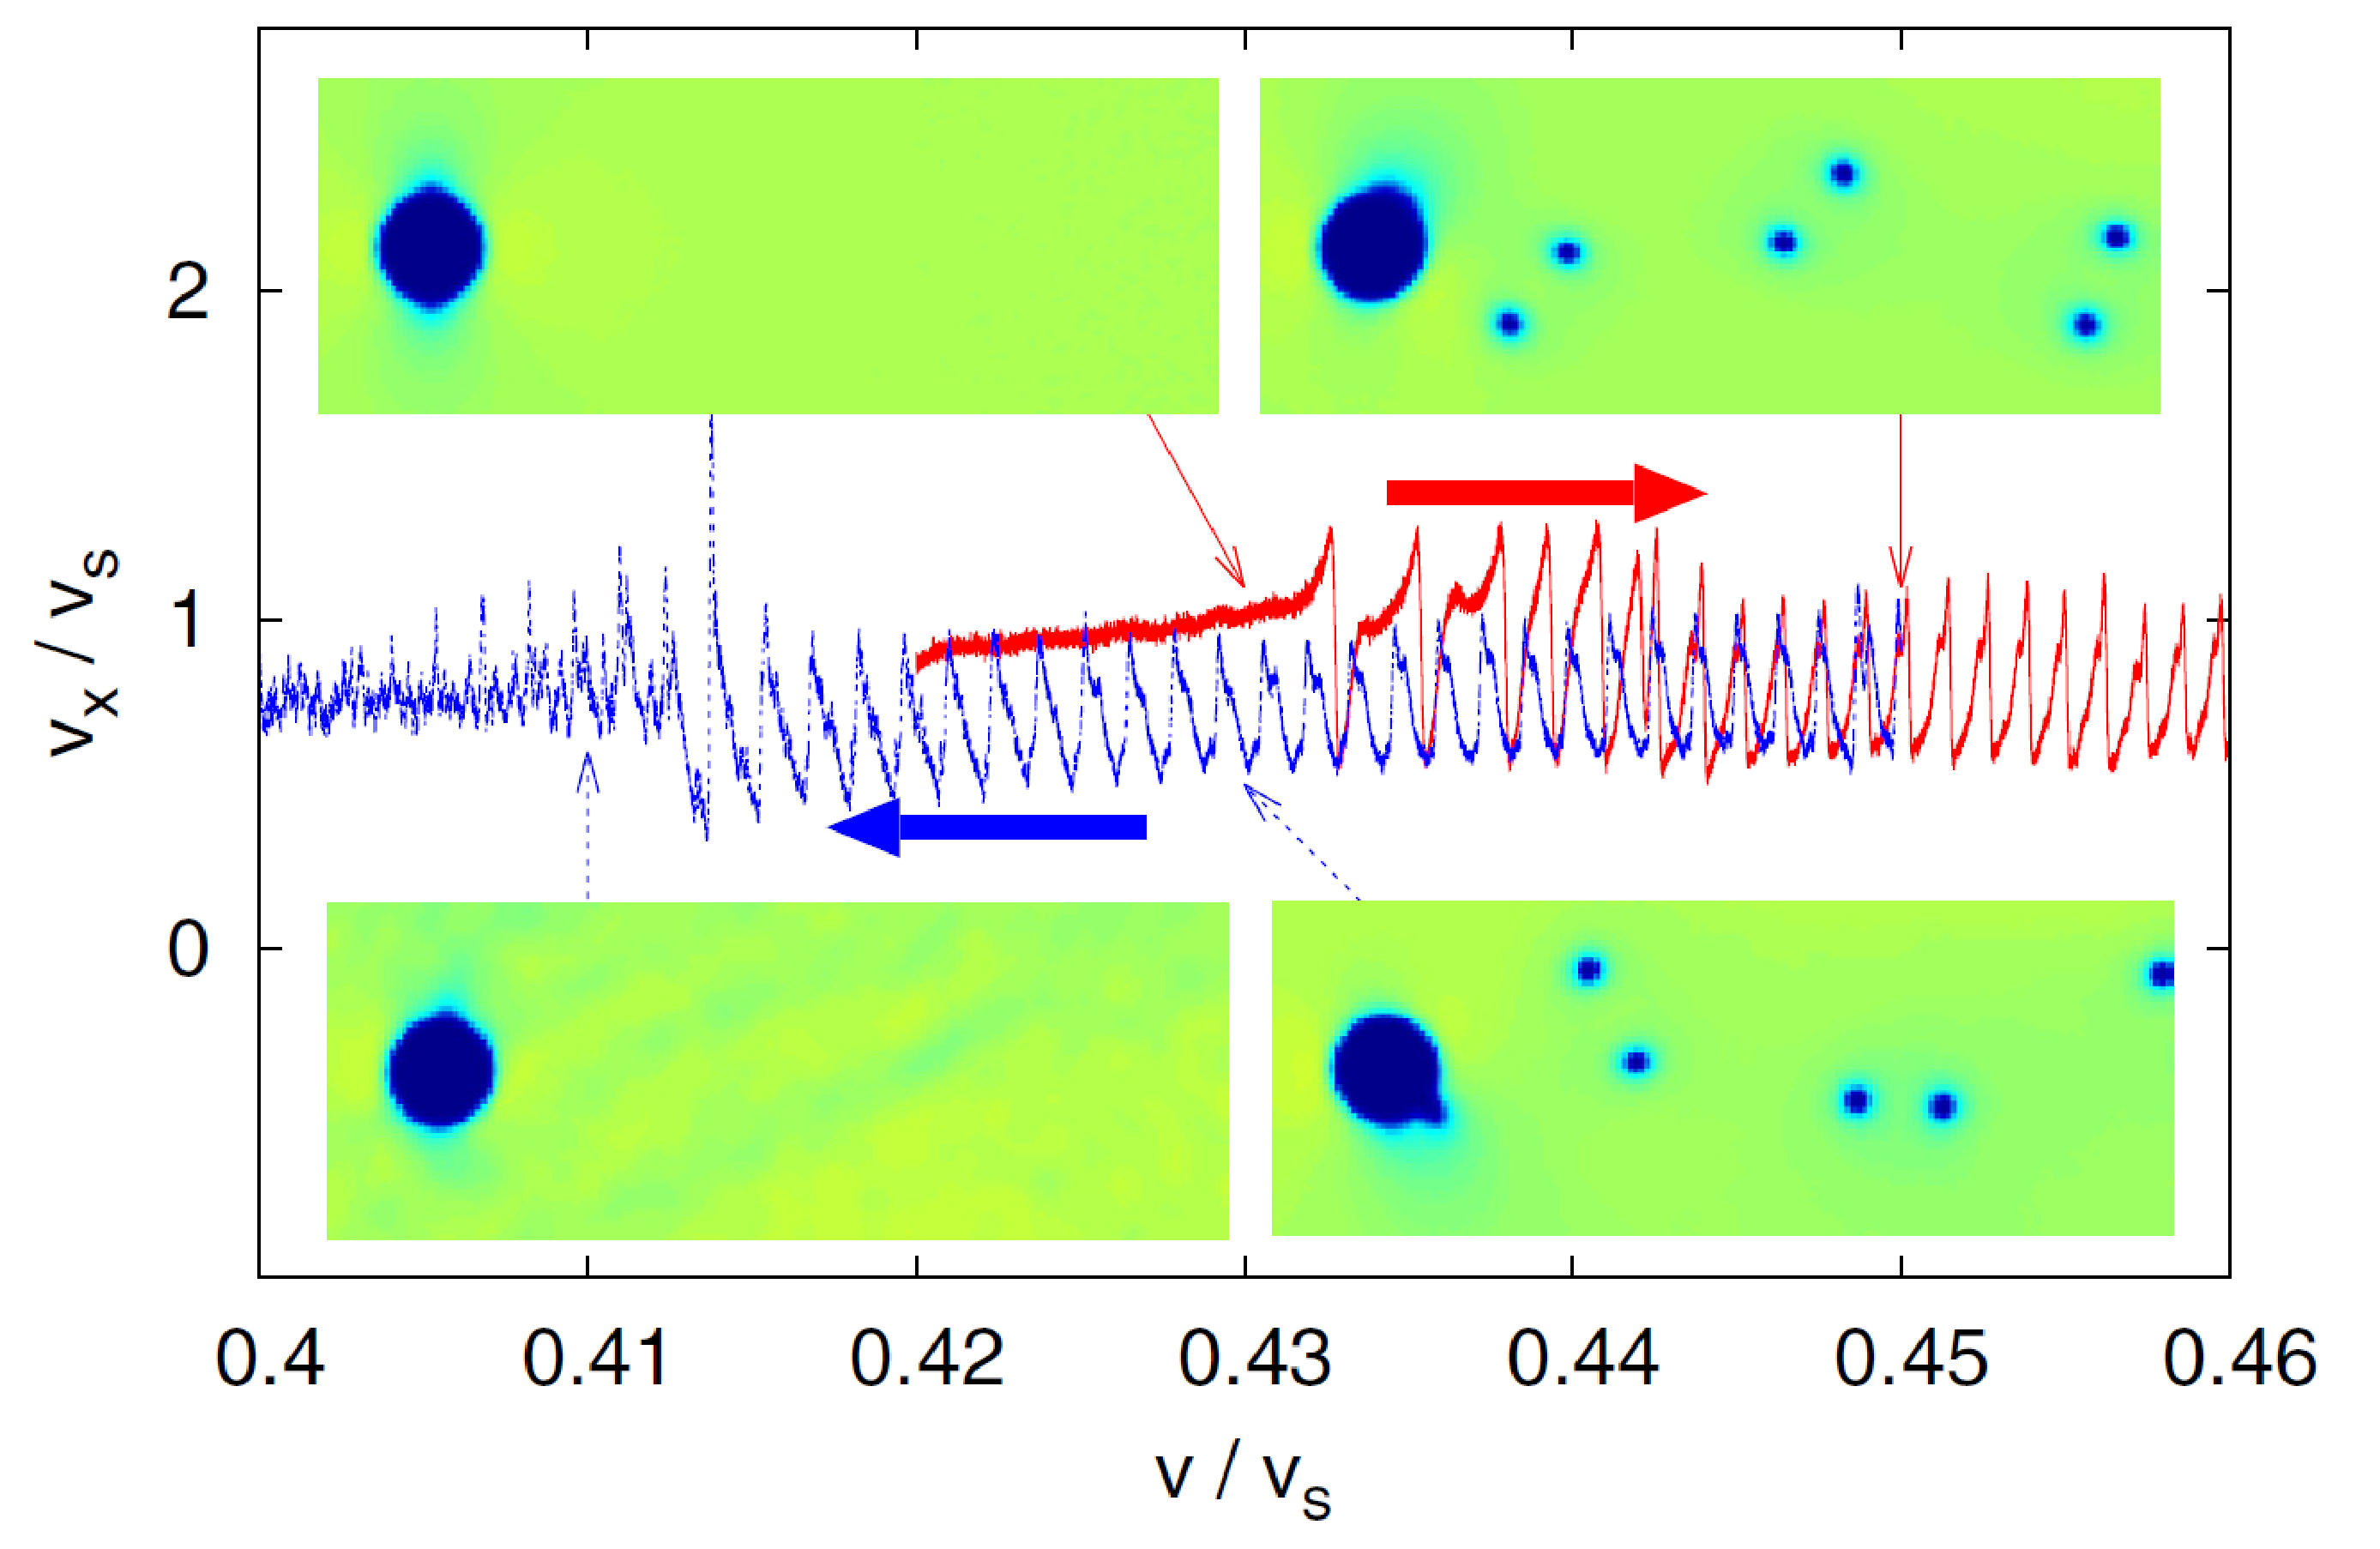
\includegraphics[scale=0.30, keepaspectratio]{4-3.eps}
\caption{
Time evolution of $v_x$ at $(x,y) = (0,R +
2 \xi)$ for $R = 4.1 \xi$ . The velocity is increased as $V(t)/v_s = 0.42 +
10^{-5}t/ \tau$ (red, solid line) or decreased as $V(t)/v_s = 0.45-10^{-5}t/\tau$
(blue, dashed line). The insets show the density profiles at $V(t)/v_s =
0.43$ and $0.45$ for the increase in $V(t)$, and $0.43$ and $0.41$ for the
decrease in $V(t)$.
}
\label{FIG:4-3}
\end{center}
\end{figure}
\begin{figure}[htbp]
\begin{center}
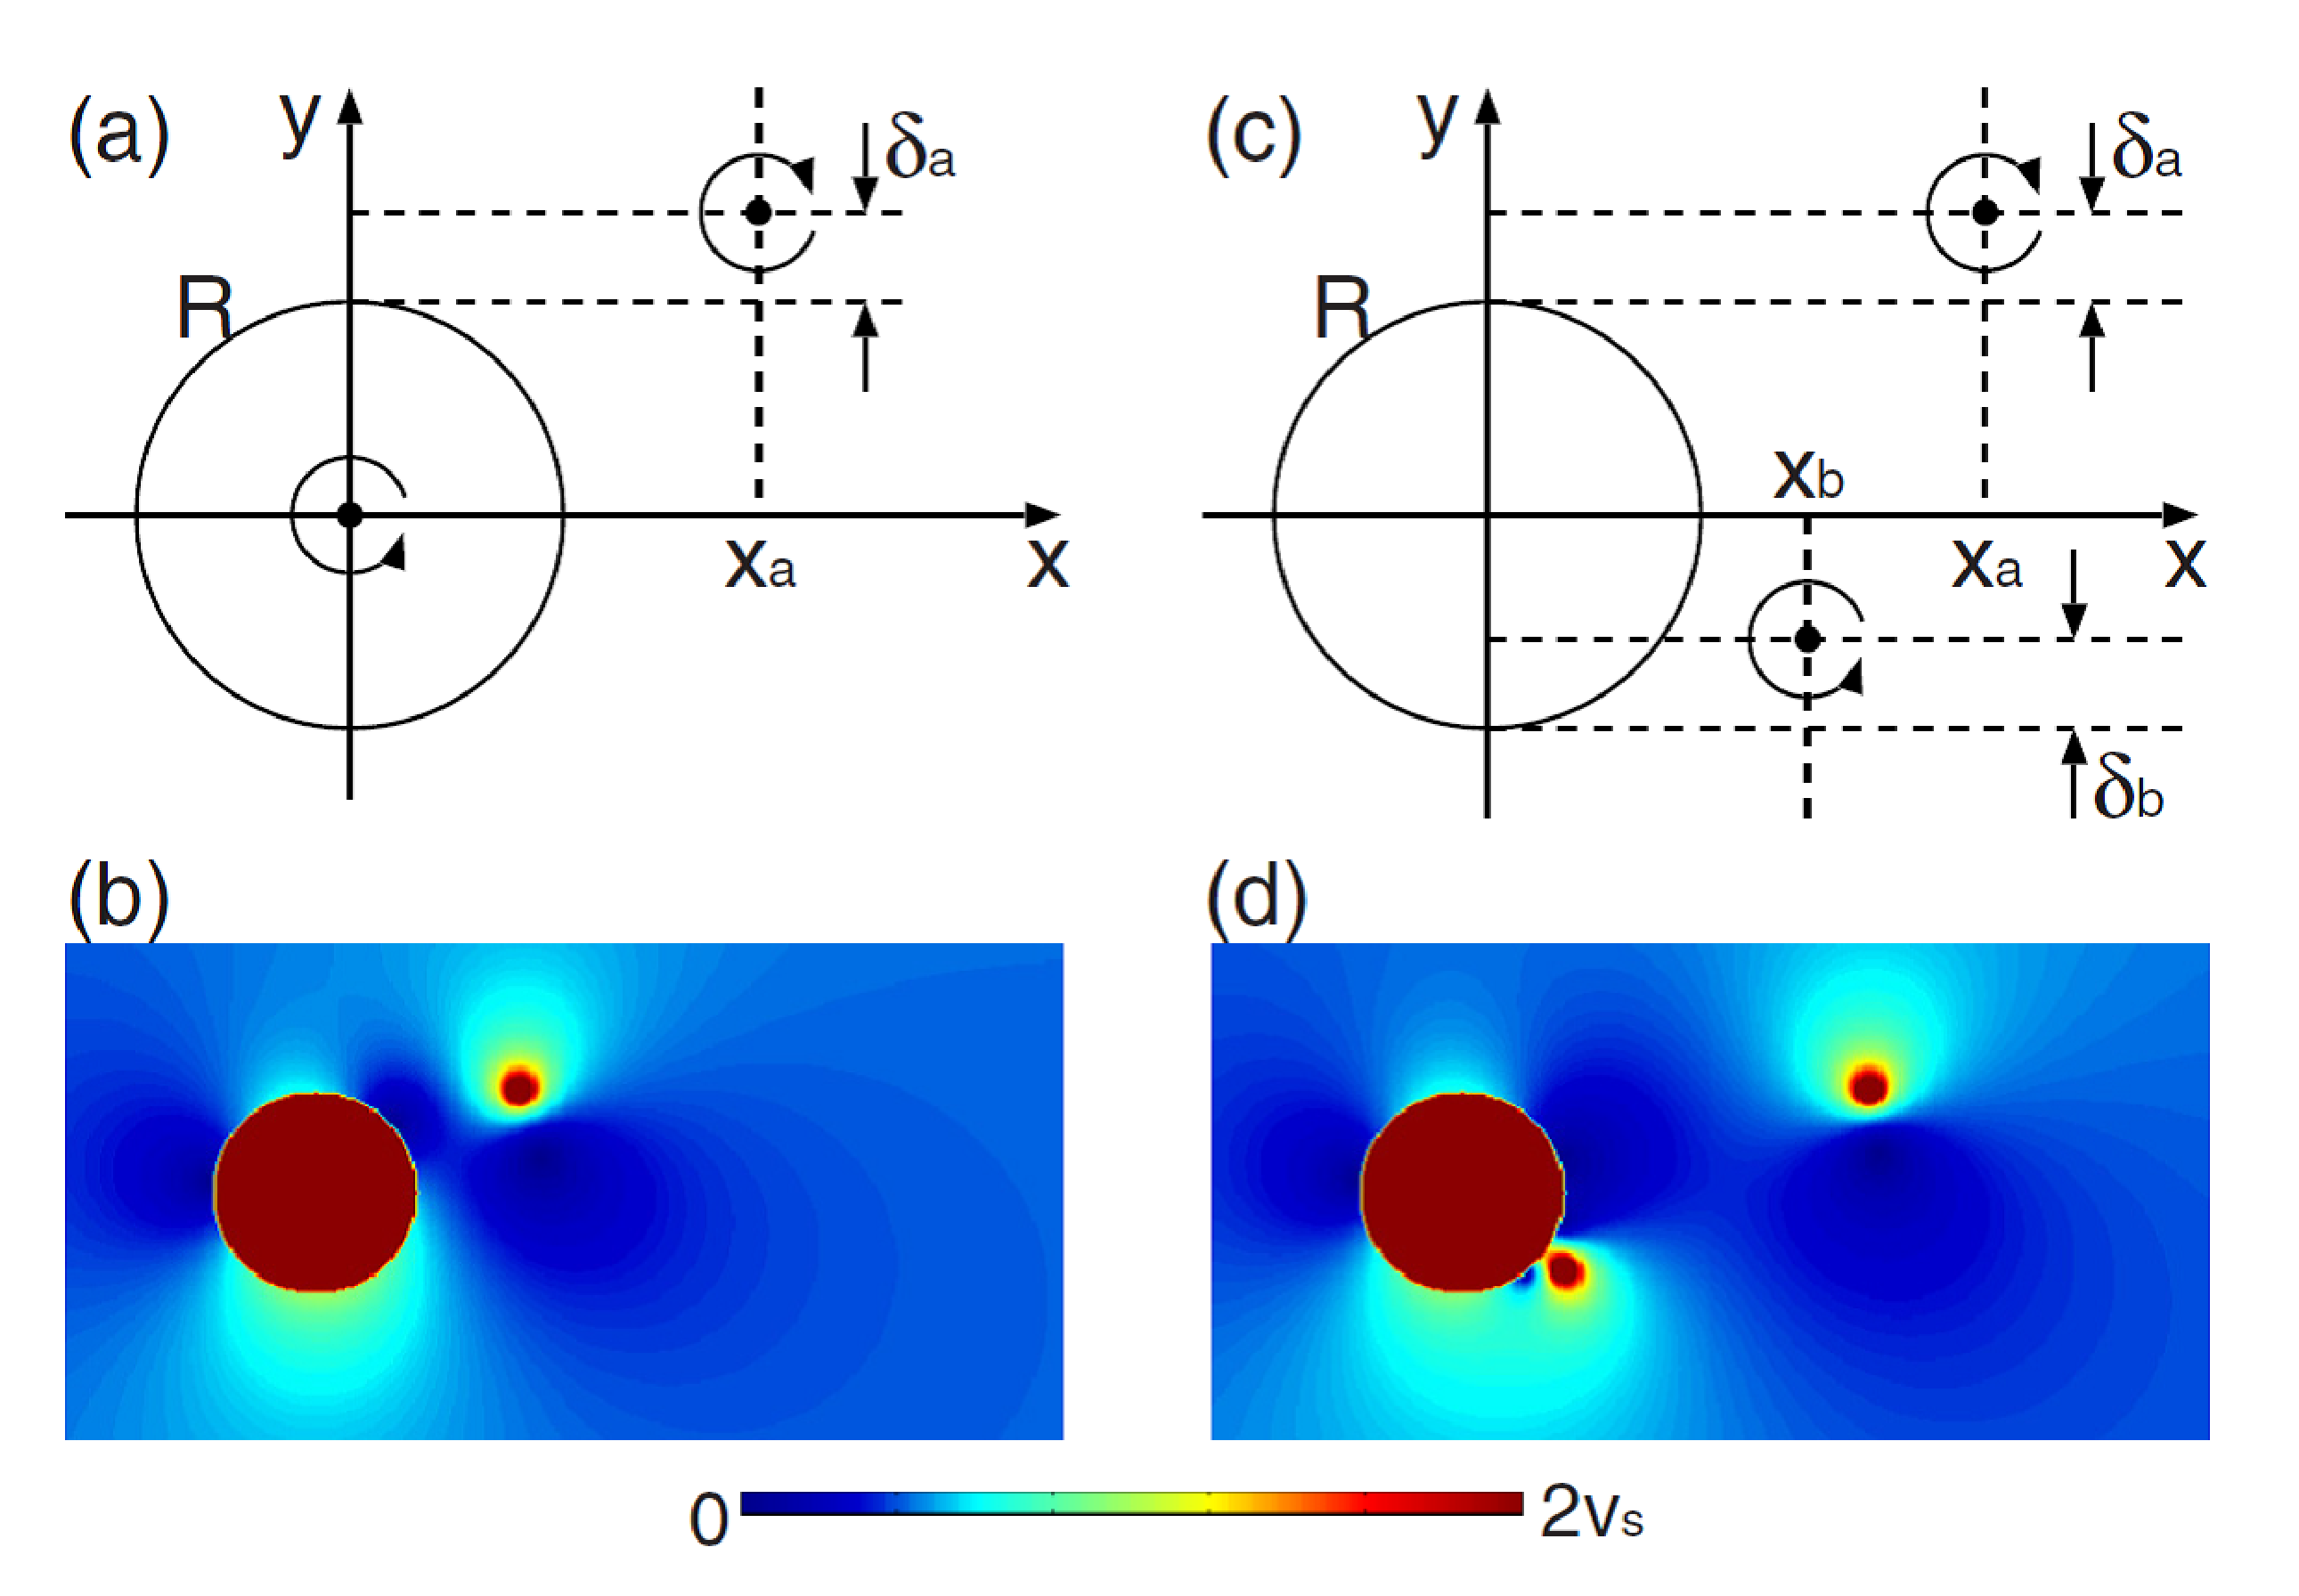
\includegraphics[scale=0.30, keepaspectratio]{4-4.eps}
\caption{
(a) and (c) Schematic illustrations of the point-vortex
model used to derive Eqs.(4.13) and (4.15), respectively. (b) $|\vec{v}|$
in Eq.(4.13) for $x_a = 2R$ and $\delta_a = 0$. (d) $|v|$ in Eq. (4.15) for $x_a = 4R$,
$x_b = R, \delta_a = 0,$ and $\delta_b = \xi$ . The size of each panel in (b) and (d) is
$40 \xi \times 20 \xi$.
}
\label{FIG:4-4}
\end{center}
\end{figure}
\ To show the hysteresis clearly, we gradually increase
and decrease the velocity $V(t)$ around the critical
velocity. Figure 4.3 shows the time evolution of the flow
velocity $v_x$ at $(x,y) = (0, R+2\xi)$. When the velocity $V(t)$
is gradually increased, the vortex shedding starts at the critical
velocity $V_{c1} \simeq 0.432 v_s$. On the other hand, when $V(t)$
is decreased from above $V_{c1}$, the periodic vortex shedding
continues for $V(t) < V_{c1},$ eventually stopping at the
lower critical velocity $V_{c2} \simeq 0.412 v_s$. The fluctuation
in $v_x$ for $V(t) \lesssim 0.41 v_s$, is due to remnant disturbing
waves.
\\
\ The velocity field around a circular obstacle can be
analyzed using the point-vortex model for an inviscid
incompressible fluid. The situation in Fig. 4.2(c) is modeled
an in Fig. 4.4(a), where a clockwise vortex is located at
$(x,y)=(x_a, R+\delta_a)$ and the circle of radius $R$
contains a counter-clockwise vortex. The complex velocity
field in which the normal component $\vec{v} \cdot \vec{r}$
vanishes at $r = R$ is given by
\begin{eqnarray}
v_x - iv_y & = &
V \left( 1 - \frac{R^2}{z^2} \right)
+ \frac{\Gamma}{2 \pi i}
\left( - \frac{1}{z - z_a} + \frac{1}{z - z^\prime_a} \right),
\end{eqnarray}
where $z = x + iy, \ \Gamma = h/m, \ z_a = x_a + i(R + \delta_a),$
and $z^\prime_a = R^2/z^*_a$ \cite{56}.
The first term on the right-hand side of Eq.(4.13)
approaches a uniform flow $(v_x, v_y)=(V,0)$ at
infinity $|z| \rightarrow \infty$ and the second term
represents a flow generated by the vortices located at
$z_a$ and the origin.
\\
\ The flow velocity at $z = \pm iR$ is
\begin{eqnarray}
v_x & = & 2V \mp \frac{\Gamma}{2 \pi}
\frac{x^2_a + \delta_a(2R+\delta_a)}{x^2_a + (R \mp R + \delta_a)^2}
\end{eqnarray}
and $v_y = 0$, which indicates that the flow velocity at
$z \simeq -iR$ is enhanced by the vortices. Thus, once a vortex
is released from $z \simeq iR,$ the next vortex is created at
$z \simeq -iR,$ which results in the dynamics shown in Fig .4.2(d).
The velocity field in Eq.(4.13) for $x_a = 2R$ and $\delta_a = 0$ is
shown in Fig. 4.4(b), which is very similar to Fig. 4.2(c).
\\
\ The situation in Fig. 4.2(d) is modeled by Fig. 4.4(c), for
which the velocity field is given by
\begin{eqnarray}
v_x - iv_y & = & V \left( 1 - \frac{R^2}{z^2} \right)
+ \frac{\Gamma}{2 \pi i} \left( - \frac{1}{z-z_a} + \frac{1}{z-z^\prime_a}
+ \frac{1}{z-z_b} - \frac{1}{z-z^\prime_b} \right),
\end{eqnarray}
where $z_b = x_b + i(-R+\delta_b)$ and $z^\prime_b + R^2/z^*_b$. The flow
velocity at $z=-iR$ is
\begin{eqnarray}
v_x & = & 2V + \frac{\Gamma}{\pi}
\left[
\frac{\delta_b}{x^2_b+\delta^2_b} - \frac{2R+\delta_a}{x^2_a+(2R+\delta_a)^2}
\right].
\end{eqnarray}
When $\delta_b$ is positive, the first term in the square bracket
of Eq.(4.16), i.e., the vortex at $z=z_b,$ enhances the flow
velocity. The vortex released from $z \simeq -iR$ therefore induces
the creation of the subsequent vortex at $z \simeq -iR$.
The velocity field in Eq.(4.15) for $x_a=4R,\delta_a=0,x_b=R,$
and $\delta_b=\xi$ is shown in Fig. 4.4(b), which well reproduces
Fig. 4.2(d).Thus, vortices shed behind an obstacle induce
the creation of an additional vortex, resulting in periodic
vortex shedding, and ultimately hysteretic mechanism
that allows this behavior to continue below the critical velocity $V_{c1}$.
\\
\ Figure 4.5 shows the radius $R$ and the velocity $V$ dependence
of the flow patterns. The vortex shedding always
occurs in the "vortex shedding" region and vortices are
never created in the "no vortex" region. The "bistability"
region lies between these two regions, in which a stationary laminar
flow is stable.However periodic vortex shedding is
kept once it starts.For $R \lesssim 2 \xi,$ the bistability region
disappears, probably because $\delta_b \sim R$ in Eq.(4.16) is small and
hence the enhancement of successive vortex creation
is less effective. Although the instability region may also
exist for $R \gtrsim 10\xi,$ it is difficult to determine the precise
value of $V_{c2}$ numerically, since the vortex shedding dynamics
are periodic for large $R$, and are dependent on
infinitesimal numerical noises.
\begin{figure}[htbp]
\begin{center}
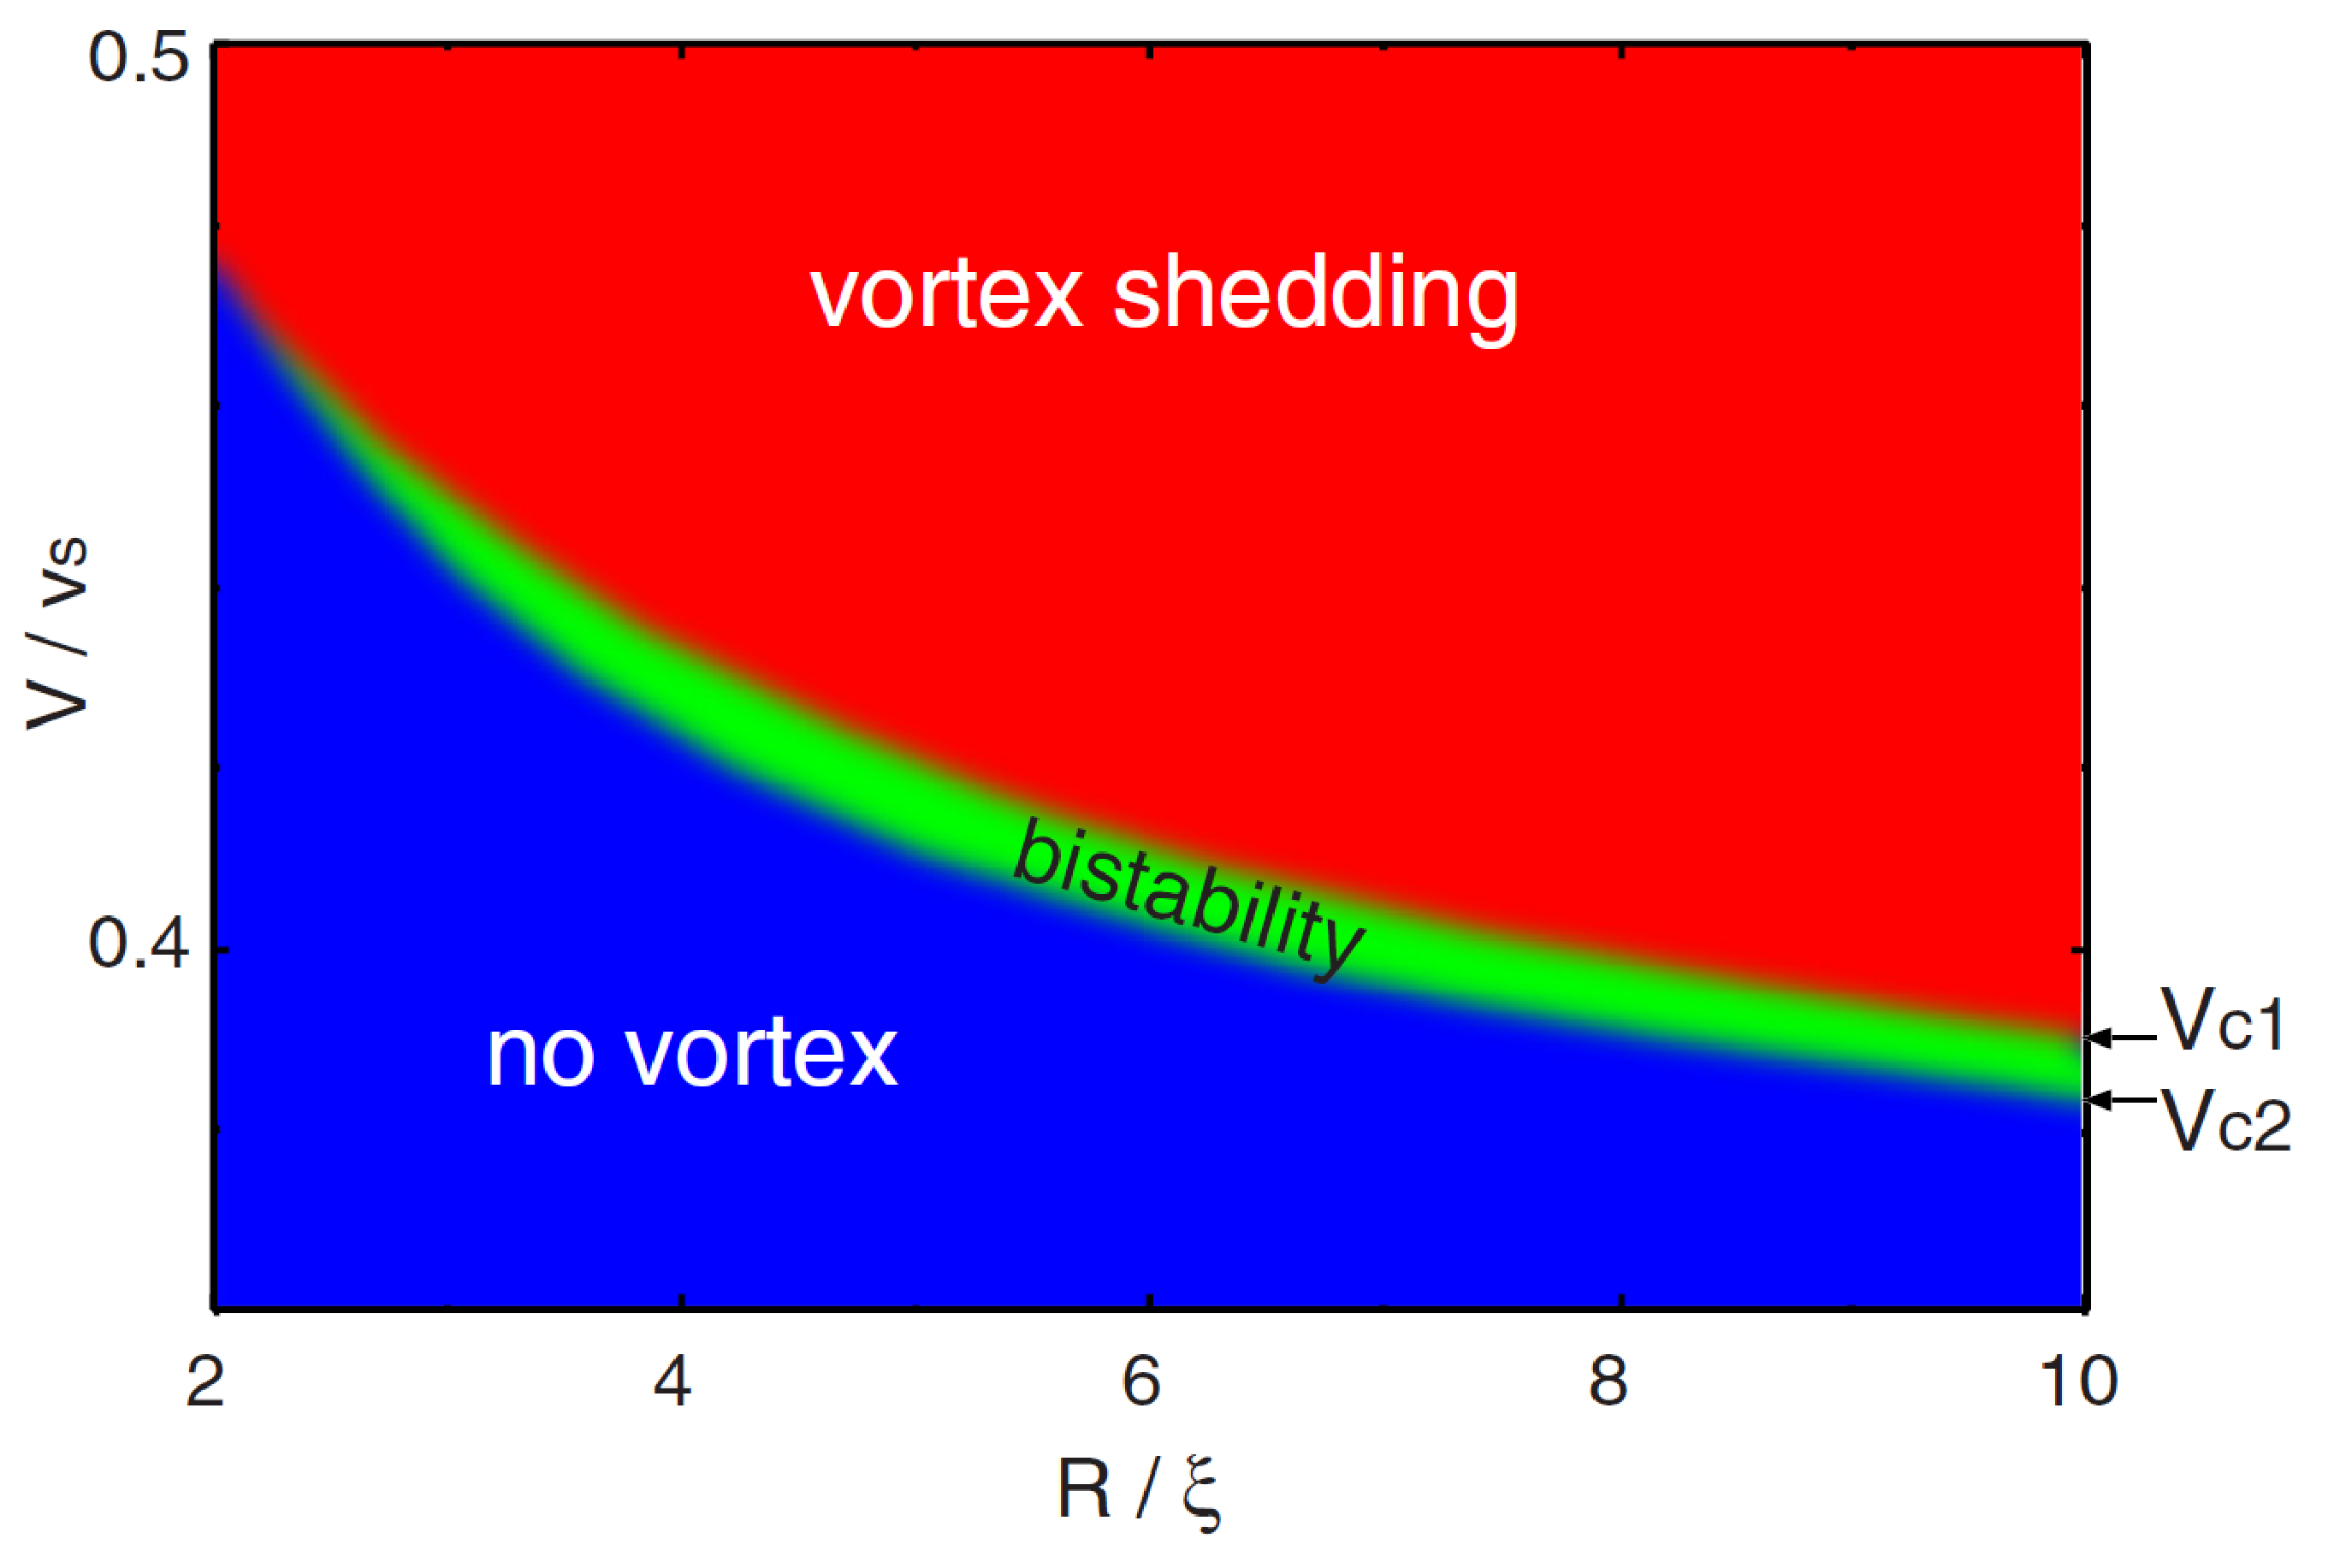
\includegraphics[scale=0.30, keepaspectratio]{4-5.eps}
\caption{
Parameter diagram with respect to the
obstacle radius $R$ and the velocity $V$. The vortex shedding always
occurs in the "vortex-shedding" region, no vortices are created in the
"no vortex" region, and hysteresis appears in the "bistability" region.
The boundaries between the bistability and vortex-shedding regions
and the bistability and no-vortex regions are $V_{c1}$ and $V_{c2}$, respectively.
}
\label{FIG:4-5}
\end{center}
\end{figure}
\subsection{Three dimensional system}
\ Next we examine a 3D system. We use a Gaussian
potential for the moving obstacle as
\begin{eqnarray}
u ( \vec{r} ) & = & 100 \mu e^{-0.15 \left(x^2+y^2+z^2 \right) / \xi^2}
\end{eqnarray}
A spherical rigid potential analogous to that in Eq.(4.10)
gives similar results. We prepare the initial state of a stationary
laminar flow with $V=0.6v_s,$ which is below the
critical velocity $V_{c1} \simeq 0.601$ for vortex creation. In order
to trigger the vortex shedding, an additional potential
\begin{eqnarray}
u_{{\rm add}} (\vec{r}) & = & 0.2\mu e^{-0.6 \left[x^2+(y-d)^2+z^2 \right] / \xi^2}
\end{eqnarray}
is applied during $400 \tau < t < 420 \tau,$ where $d=6.3 \xi$. This
additional potential is located at the edge of the potential
$u$ in Eq.(4.17), triggering the generation of a quantized
vortex ring, as shown in Fig. 4.6(b). Subsequent vortex
creation is induced and periodic vortex shedding begins,
as shown in Figs. 4.6(c) and 4.6(d), respectively. This
result indicates that the bistability between the stationary
laminar flow and periodic vortex shedding also exists in
a 3D system.
\\
\ We note that the vortex rings in a 3D system are topologically
different from the vortex pairs in a 2D system. A
vortex-antivortex pair in a 2D system corresponds to a vortex
ring in a 3D system since they propagate without changing
their shapes. By contrast, a vortex-vortex pair in a 2D system,
such as that seen in Fig. 4.2(e), has no counterpart in a 3D system
since two vortices rotate around one another for a vortex-vortex
pair. Such rotation would tangle vortex rings in a 3D system.
It is interesting that both 2D and 3D systems exhibit bistability
despite the topological difference.
\begin{figure}[htbp]
\begin{center}
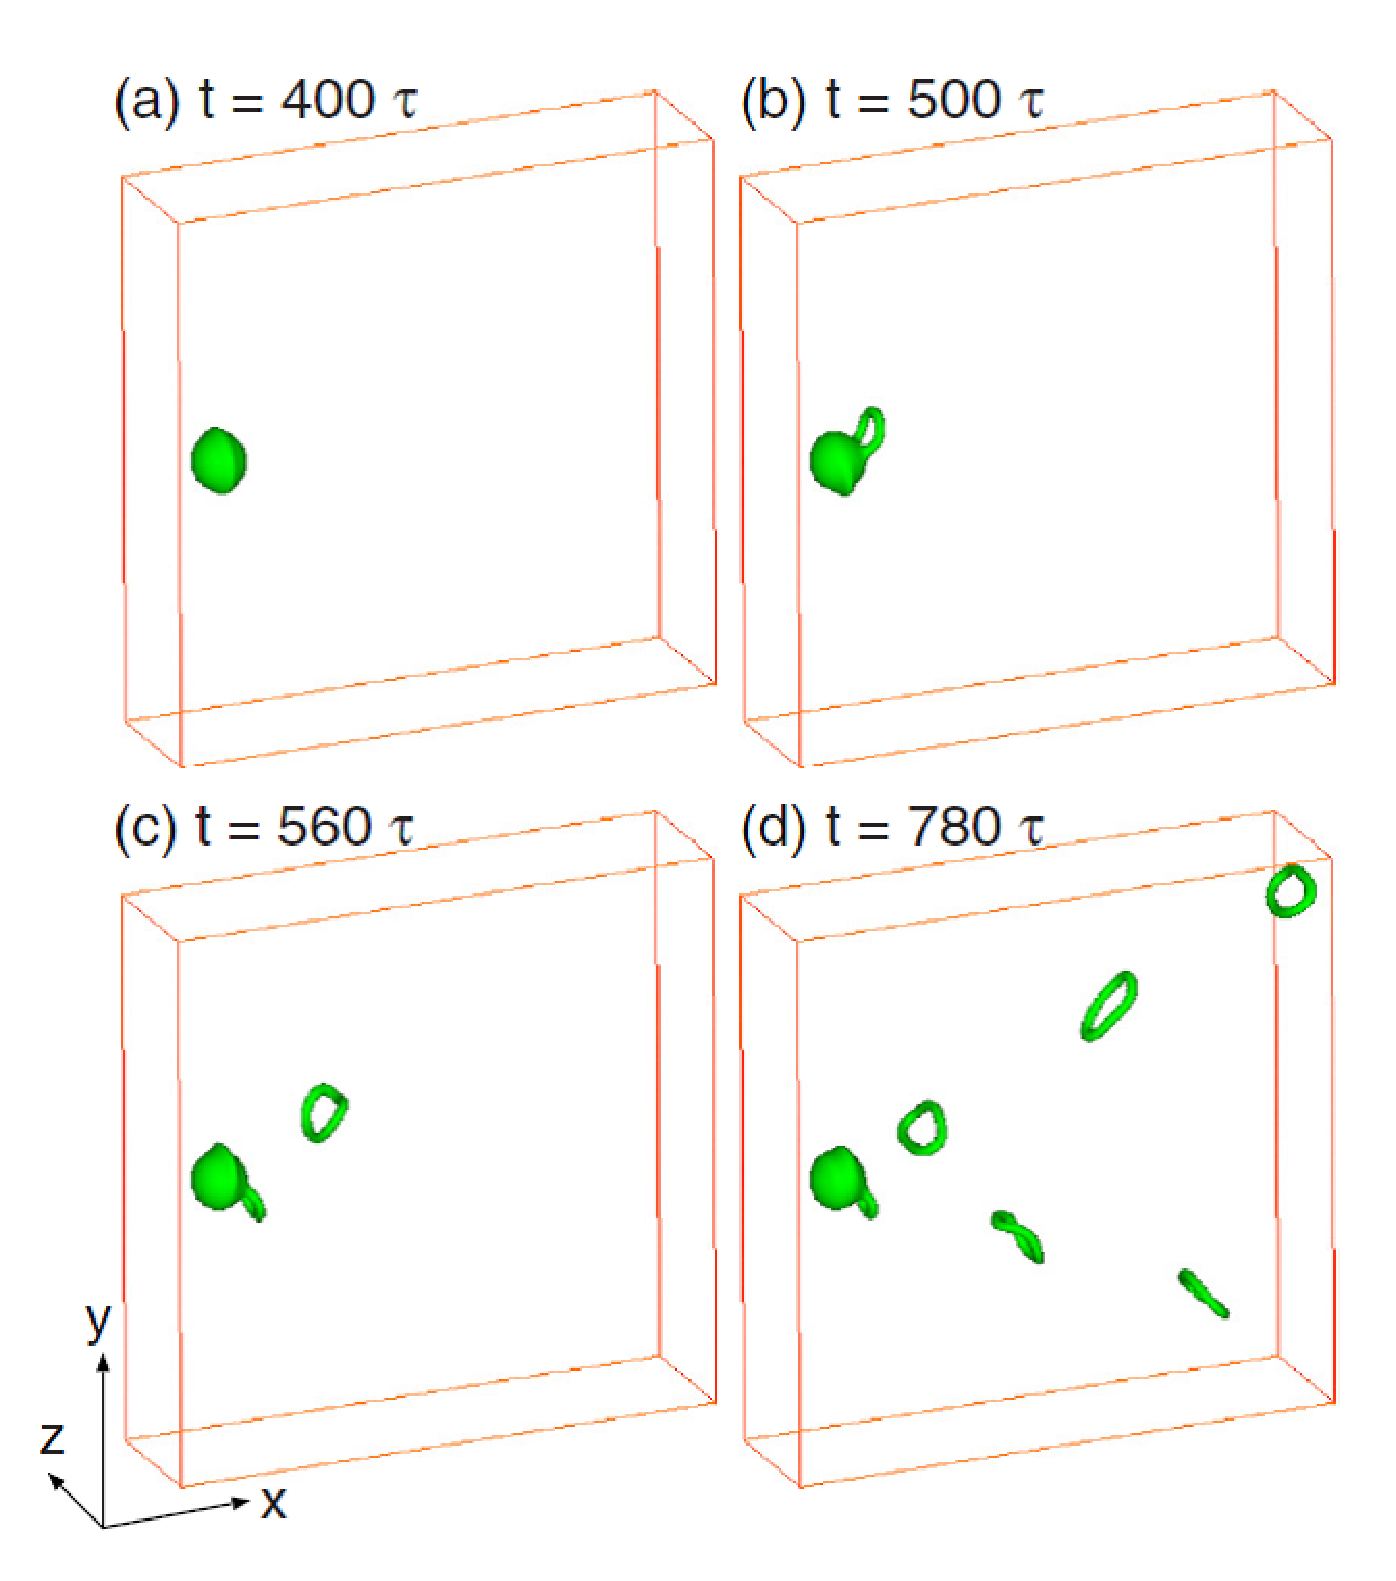
\includegraphics[scale=0.55, keepaspectratio]{4-6.eps}
\caption{
Isodensity surfaces for the 3D dynamics.
The Gaussian potential given by Eq. (4.17) moves in the $-x$ direction
at a velocity $V=0.6v_s$; the dynamics are given in the frame of
reference of the potential. An additional potential given by Eq. (4.18)
is applied during $400 \tau < t < 420 \tau$. The size of the cuboidal frame
is $126.4 \xi \times 126.4 \xi \times 31.6 \xi$.
}
\label{FIG:4-6}
\end{center}
\end{figure}

\section{Conclusion}
\ We investigated the dynamics of a BEC with a moving
obstacle potential, and found bistability between stationary
laminar flow and periodic vortex shedding. When the velocity
of the obstacle is gradually increased, quantized vortex
shedding starts at the critical velocity $V_{c1}$. On the other hand,
when the velocity is gradually decreased from above $V_{c1}$,
the vortex shedding stops at a velocity $V_{c2}$. We found that
$V_{c1} > V_{c2}$ for an appropriately sized obstacle potential Fig. 4.3.
For a velocity $V_{c1} > V > V_{c2}$, a stationary laminar flow is
stable,but periodic vortex shedding is maintained once it starts
[FIGs.4.1 and 4.2]. Such hysteretic behavior originates from the
fact that the vortices released behind the obstacle enhance the
velocity field around the obstacle, inducing subsequent vortex
generation Fig. 4.4. The bistability between the stationary
laminar flow and periodic vortex shedding exists not only in
2D systems but also in 3D systems Fig. 4.6.
We have studied the hysteretic phenomena in infinite
homogeneous systems in this chapter. To observe the hysteresis
in a trapped BEC experimentally, an elongated trap, as
in Ref.\cite{57}, is needed to move the potential through the
condensate over a long distance.
Alternatively, a large toroidal trap may be suitable for
this purpose, since the potential can be moved around the
circumference.

\chapter{Rayleigh-Taylor instability in a two-component BEC}
\section{Introduction}
\ The Rayleigh-Taylor instability(RTI) \cite{58}\cite{59}\cite{60}\cite{61} is the instability of an interface between
two fluids in a meta-stable state.

For instance, when a layer of a heavy fluid is laid on a light fluid,
the system is energetically unfavorable, and the two fluids tend to exchange their positions.
However, if the two fluids are immiscible and their interface is flat,
the exchange cannot occur without breaking the translation symmetry of the interface.
Once an infinitesimal modulation arises on the interface,
it exponentially grows due to the RTI,
and the interface develops into complicated patterns,
such as a mushroom-shaped pattern.
Such phenomena are found through nature on a wide scale,
ranging from laboratory to astronomical scales.
Recently, these kinds of interfacial instabilities have been
studied for a system of two-component Bose-Einstein condensate(BEC) \cite{62}\cite{63}\cite{64}\cite{65}.
\\
\ The RTI is a symmetry-breaking phenomenon, that is,
even when the interface has symmetry
(e.g., the translation symmetry of a flat interface and the rotational symmetry
of a spherical interface), an infinitesimal modulation grows
exponentially, and the symmetry is spontaneously broken.
The RTI with rotational symmetry breaking is an important subject,
occurring in a variety of systems:
e.g., exploding supernovas \cite{66}\cite{67}\cite{68},
imploding targets in inertial-confinement fusion \cite{69},
and collapsing cavitation bubbles \cite{70} \cite{71}.
In this chapter, we study the rotational-symmetrybreaking RTI
in a trapped two-component BEC.
Systems of trapped BECs that have so far been proposed for observing the RTI
are a tight,
pancake-shaped system in which the two components separate into two semicircular shapes \cite{62}
and a cigar-shaped system in which a two-component BEC forms a domain
structure in the axial direction \cite{63}.
In these systems, however, the symmetry-breaking RTI cannot be observed since
the relevant symmetry is broken from the initial state due to the inhomogeneity of the trapped systems.
In contrast, in this chapter, we propose trapped systems that explicitly show the symmetry-breaking RTI.
\\
\ We consider a two-component BEC with rotational symmetry in which the two components separate radially and
the inner component is surrounded by the shell of the outer component.
The interface between the two components has a spherical shape for a spherically symmetric trap
and a circular shape for a quasi-two-dimensional axisymmetric trap.
If we change a parameter in such a way that the inner component tends to go out of
the outer shell component,
the RTI breaks the rotational symmetry of the interface, and the spherical or
circular interface is deformed into various patterns.
The symmetry-breaking RTI can thus be realized in a trapped BEC.
%\\
%\ This study is organized as follows. Section 2 provides a formulation of the problem,
%and Sec. 3 shows numerical results.
%Section 3

\section{Formulation of the problem}
\ We consider a mixture of two kinds of bosonic atoms with
masses $m_1$ and $m_2$ confined in trapping potentials $V_1$ and
$V_2$, respectively. In the mean-field theory, the system is described
by the two-component Gross-Pitaevskii(GP) equation $(j \neq j^\prime)$
\begin{eqnarray}
i \hbar \frac{\partial \psi_j}{\partial t} =
\left(
- \frac{\hbar^2}{2m_j} \nabla^2 + V_j + g_{jj} |\psi_j|^2 + g_{jj^\prime} |\psi_{j^\prime}|^2
\right) \psi_j,
\end{eqnarray}
where $\displaystyle g_{jj^\prime} = \frac{2 \pi \hbar^2 a_{jj^\prime}}{m_j}
+\frac{2 \pi \hbar^2 a_{jj^\prime}}{m_j^\prime}$ with $a_{jj^\prime}$ being the
$s$ wave-scattering length between the atoms in components $j$ and $j^\prime$.
The macroscopic wave function $\psi_j$ is normalized as $\int |\psi_j|^2 \diff \vec{r} = N_j$
with $N_j$ being the number of atoms in component j. The two components are miscible for
$g_{11}g_{22} > g_{12}^2$ and immiscible for $g_{11}g_{22} < g_{12}^2$.
\\
\ We solve the three dimensional(3D) GP equation in Eq.(5.1)
numerically, using the pseudo-spectral method \cite{34}. The initial
state is the ground state prepared by the imaginary-time-propagation method
in which $i$ on the left-hand side of Eq.(1) is replaced by -1. We then add a small noise to
the initial state as a seed that triggers the RTI. The dynamics do not
depend on the initial noise qualitatively.
\\
\ In the following calculations, we assume a dual-spaces
BEC with $^{85} {\rm Rb}$ and $^{87} {\rm Rb}$, where the $|f=2, m_f = -1 \rangle$ state
of $^{85} {\rm Rb}$ is component one ad the $|f=1, m_f=-1 \rangle$ state
of $^{87} {\rm Rb}$ is component two. This system has been realized
by Papp {\it et al}.\cite{72} in which controlled phase separation
was observed by changing the $s$-wave-scattering length $a_{11}$
of $^{85} {\rm Rb}$ using a magnetic-field Feshbach resonance, which is
variable in the range $a_{11}=(50-900)a_B$ with $a_B$ being the Bohr
radius. Since $a_{22} = 99 a_B$ and $a_{12}=213a_B$, the condition for
the phase separation is satisfied for $a_{11} < 458 a_B$.


\section{Results and Discussion}
\subsection{RTI in axisymmetric oblate systems}
\ We first demonstrate the dynamics for an axisymmetric
oblate trap $\displaystyle V_j = m_j [\omega_\perp^2 (x^2+y^2)+\omega_z^2 z^2]/2$, where $\omega_z >> \omega_\perp$.
We assume that the gravitational sag is compensated and
that the two components share a common trap center. Figure 5.1
shows the time evolution of the density and phase profiles of
the system, obtained by solving the 3D GP equation in Eq.(1).
The initial state is the ground state for $a_{11} = 80 a_B$ and
$N_1 = N_2$, which has the axisymmetric circular interface between
the two components Fig. 5.1(a). The repulsive interaction
of component one (inner) is then gradually increased, and
when it exceeds that of component two (outer), the system
becomes meta-stable, i.e., the state in which component one
surrounds component two becomes energetically favorable.
At $t \simeq 80 {\rm ms}$, the axisymmetry of the system is broken, and
the interface is modulated due to the RTI Fig. 5.1(b). The
modulation of the interface subsequently grows to become a
fourfold mushroom shape Fig. 5.1(c). Quantized vortices are
generated under the caps of the mushrooms in both components
[circles in Fig. 5.1(e). When the tops of the mushrooms
reach the edge or the center of the system, a highly nonlinear
pattern is observed Fig. 5.1(d). The $n$-fold mushrooms shapes
with $n \neq 4$ are also observed, where $n$ is larger for a larger final
value of $a_{11}$.
\\
\ The dynamics also depend on the ratio between the
numbers of atoms $N_2 / N_1$. Figure 5.2 shows the dynamics for
$N_2/N_1 = 1/9$. After the repulsive interaction of component
one is increased, the RTI causes modulation at the interface
Fig. 5.2(b). Since $N_2$ is small, the ring of component two
splits into droplets that enter component one, forming small
mushrooms Fig. 5.2(c). The droplets of component two then
go toward the center and gather. Their complicated shapes
are similar to air bubbles rising in water. The Rayleigh-Taylor
"bubbles" as shown in [FIGs.5.1 and 5.2] have been studied in the
context of supernova explosions \cite{67}.

\begin{figure}[htbp]
\begin{center}
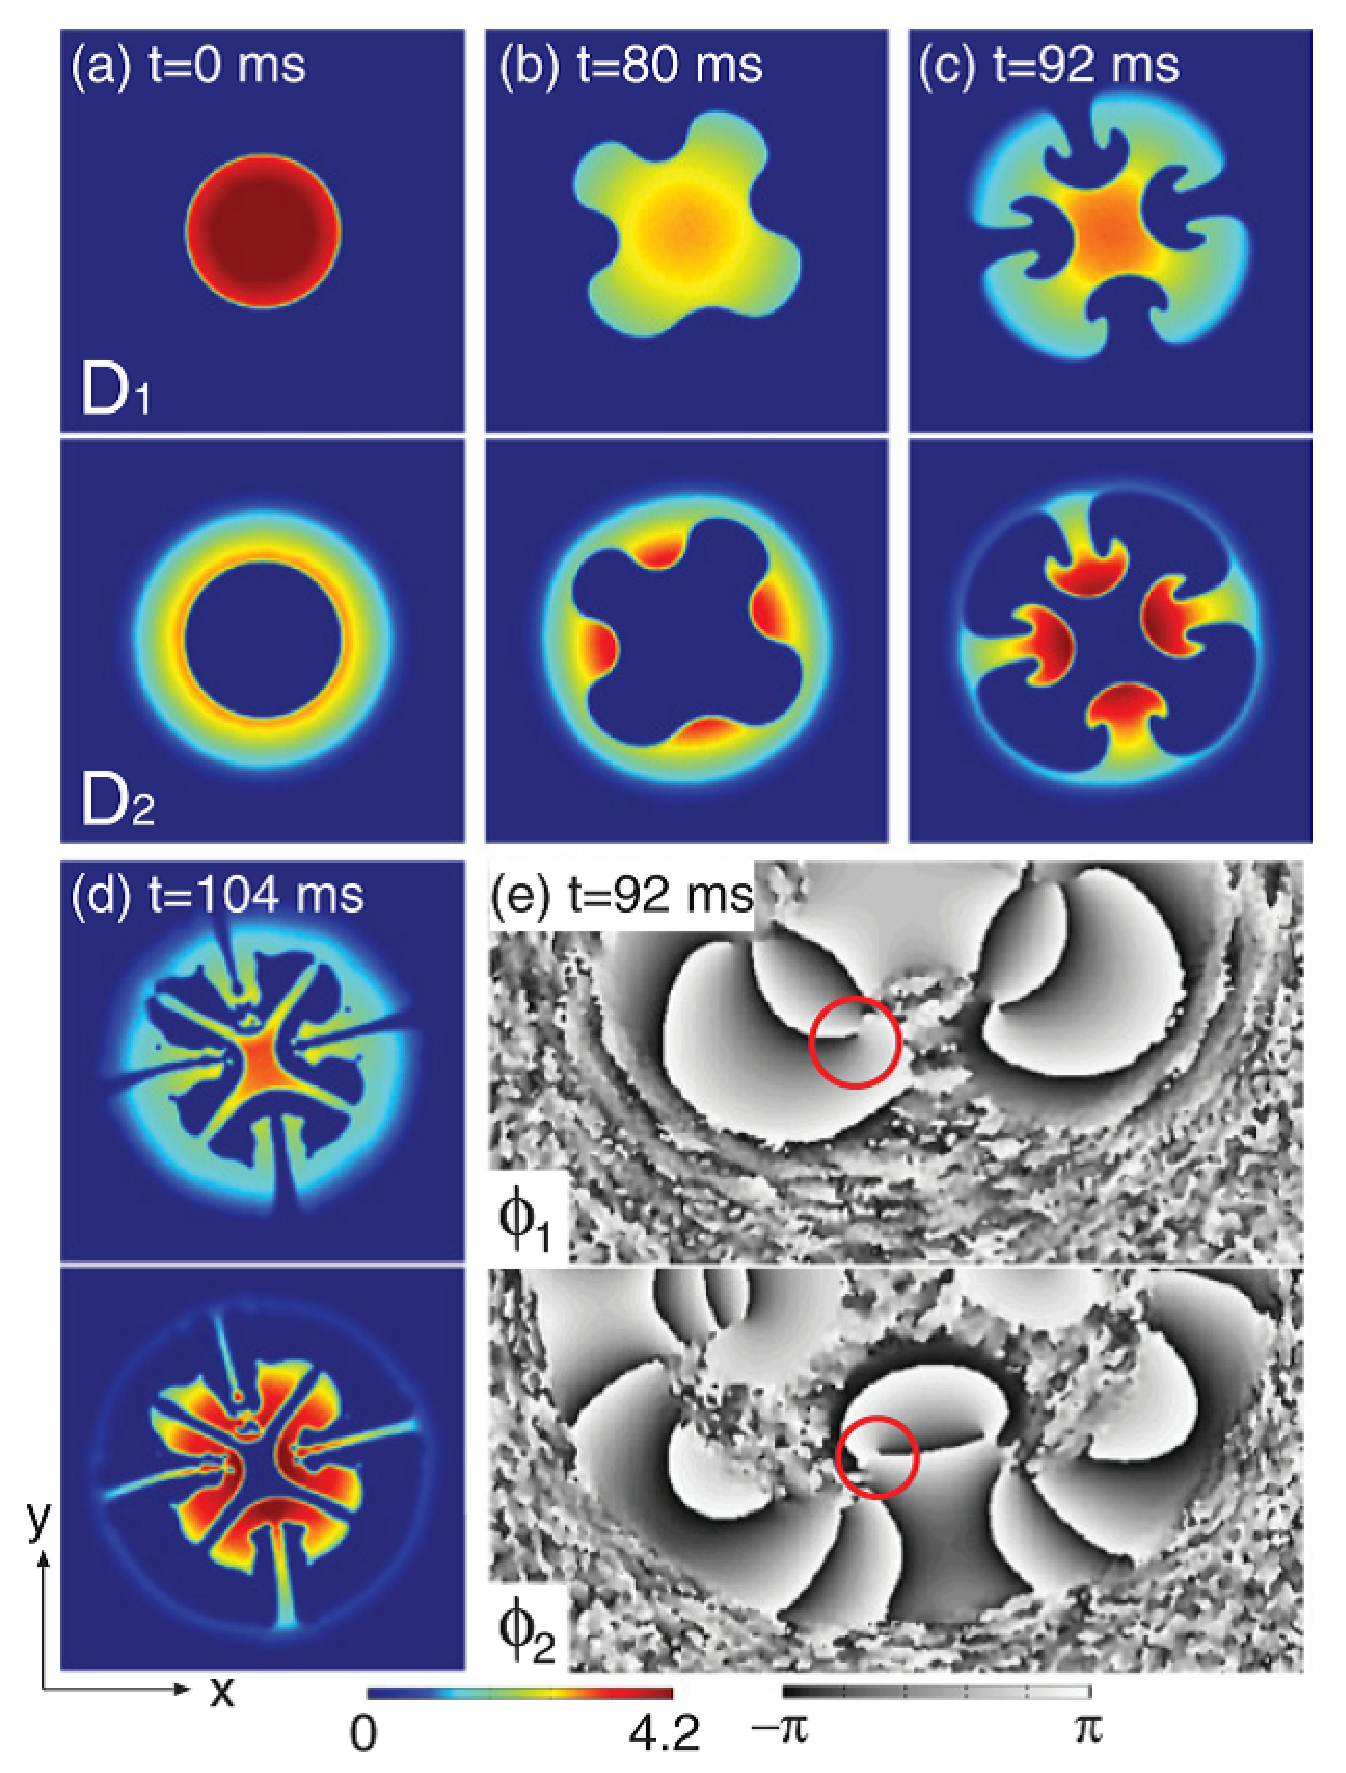
\includegraphics[scale=0.5,keepaspectratio]{5-1.eps}
\caption{(a)-(d) Dynamics of the column-density
profiles $D_1 = \int |\psi_1|^2 \diff z$(upper panels) and
$D_2 = \int |\psi_2|^2 \diff z$ (lower-panels) in an axisymmetric trap with
$( \omega_\perp , \omega_z ) = 2 \pi \times (25, 1250)$ Hz.
The scattering length $a_{11}$ is linearly increased from $80_{a_B}$ to $240_{a_B}$
between $t=0$ and $t=40$ ms, and after that $a_{11}$ is fixed to $240_{a_B}$.
The numbers of atoms are $N_1 = N_2 = 10^5$. The unit of the column density
is $10^{12} {\rm cm}^{-2}$. (e) Cross-sectional phase profile $\phi_j = \arg [\psi_j(z=0)]$
of the lower half region of (c). The circles in (e) indicate examples
of quantized vortices created under the caps of the mushrooms. The
field of view is $65.4 \times 65.4 {\rm \mu m}$ in (a)-(d) and $65.4 \times 32.7 {\rm \mu m}$ in (e).}
\label{FIG:5-1}
\end{center}
\end{figure}
\begin{figure}[htbp]
\begin{center}
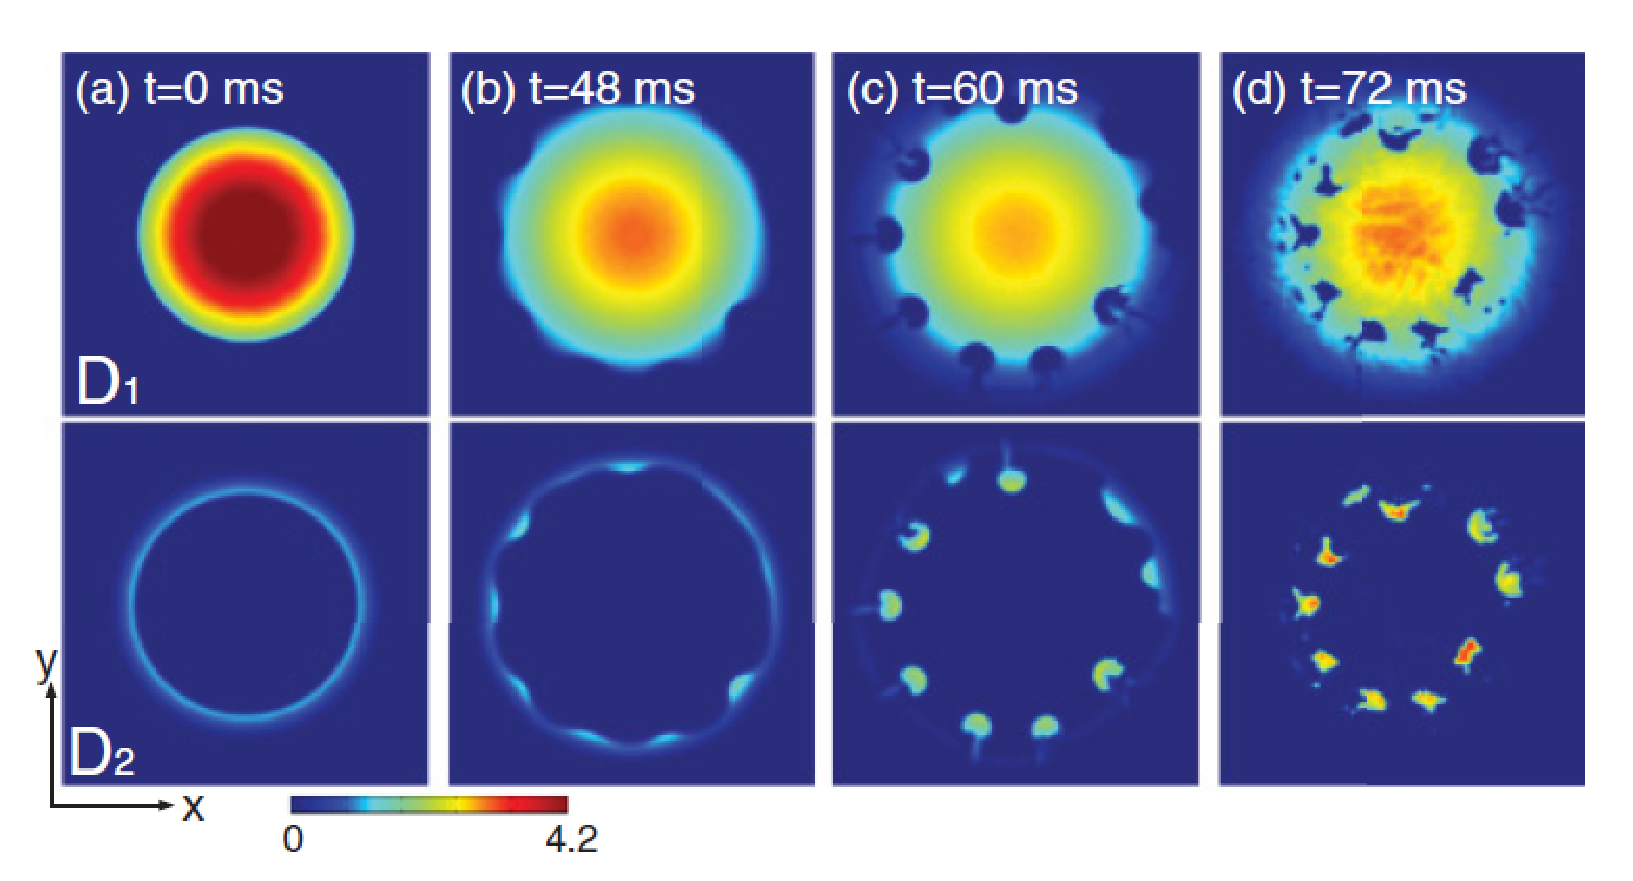
\includegraphics[scale=0.5,keepaspectratio]{5-2.eps}
\caption{
Dynamics of the column-density profiles
$D_1$ and $D_2$ for $N_1 = 1.8 \times 10^5$ and $N_2 = 2 \times 10^4$. Other parameters
and the same as those in Fig. 5.1.
}
\label{FIG:5-2}
\end{center}
\end{figure}
\subsection{RTI in a spherically symmetric system}
\ Next we consider a system confined in a spherically symmetric
trap given by $V_j = m_j \omega^2_j r^2 / 2 $ with $r^2 = x^2+y^2+z^2$.
The initial state is the ground state for $a_{11}=200 a_B$ and
$\omega_1 = \omega_2$ in which component two with a spherical shape is
surrounded by a shell of component one Fig. 5.3(a). The trap
frequency $\omega_1$ of component one is the increased gradually.
The outer component is pushed in ward by the increase in the
trap frequency, and the RTI is induced at the spherical interface.
At $t \simeq 36$ms, the RTI breaks the rotational symmetry, and
the spherical interface is modulated [FIGs.5.3(b) and 5.3(d)].
The interface is then deformed into a "mushroom ball" Fig. 5.3(e).
\\
\ The unstable modes of the interface are estimated by a
simple analysis. We assume in-viscid, in-compressible, and
irrotational fluids, and component two of a spherical bubble
with radius $R$ is surrounded by component one. The excitation
frequency $\Omega$ of the inter-facial mode proportional to the
spherical harmonics $Y_l^m (\theta, \phi)$is given by \cite{73}
\begin{eqnarray}
\Omega^2 = \frac{l(l+1)}{R[lm_1 n_1 + (l+1)m_2 n_2]}
\times \left[
n_2 f_2 - n_1 f_1 + \frac{(l-1)(l+2)}{R^2}\sigma
\right]
\end{eqnarray}
where $n_j$ is the atomic density, $f_j$ is the external force acting
on an atom at the interface, and $\sigma$ is the inter-facial-tension
coefficient. if $\Omega$ is purely imaginary, i.e., the right-hand side of
Eq.(2) is negative, the mode is dynamically unstable. Using the
expression of $\sigma$ for a two-component BEC derived in Ref.\cite{74}
and $f_j = m_j \omega_j^2 R$, we find that the modes for $l \leq l \leq 7$ are
unstable for the parameters in Fig. 5.3.See Fig. 5.3(d) for the inter-facial pattern.
\\
\ From Eq.(5.2), we find that the RTI is induced by an
increase in $\rho_1$ or $f_1$ or by a decrease in $\rho_2$ or $f_2$. The density
$\rho_1$ depends on the interaction: an increase (decrease) in $a_{jj}$
expands (contracts) component $j$, decreasing (increasing) $\rho_{j}$.
The force $f_j$ acting on each component can be controlled if
the external trapping potential for each component can be
controlled independently. The RTI can thus be induced in
several ways: for example, (i) an increase in the scattering
length of the inner component, (ii) a decrease in the trap
frequency of the inner component, (iii) a decrease in the
scattering length of the outer component, or (iv) an increase
in the trap frequency of the outer component. The dynamics
shown in [FIGs.5.1 and 5.3] correspond to (i) and (iv), respectively.
We have numerically confirmed that the RTI can be observed
for all the methods (i)-(iv) for both axisymmetric oblate traps
and spherically symmetric traps.
\begin{figure}[htbp]
\begin{center}
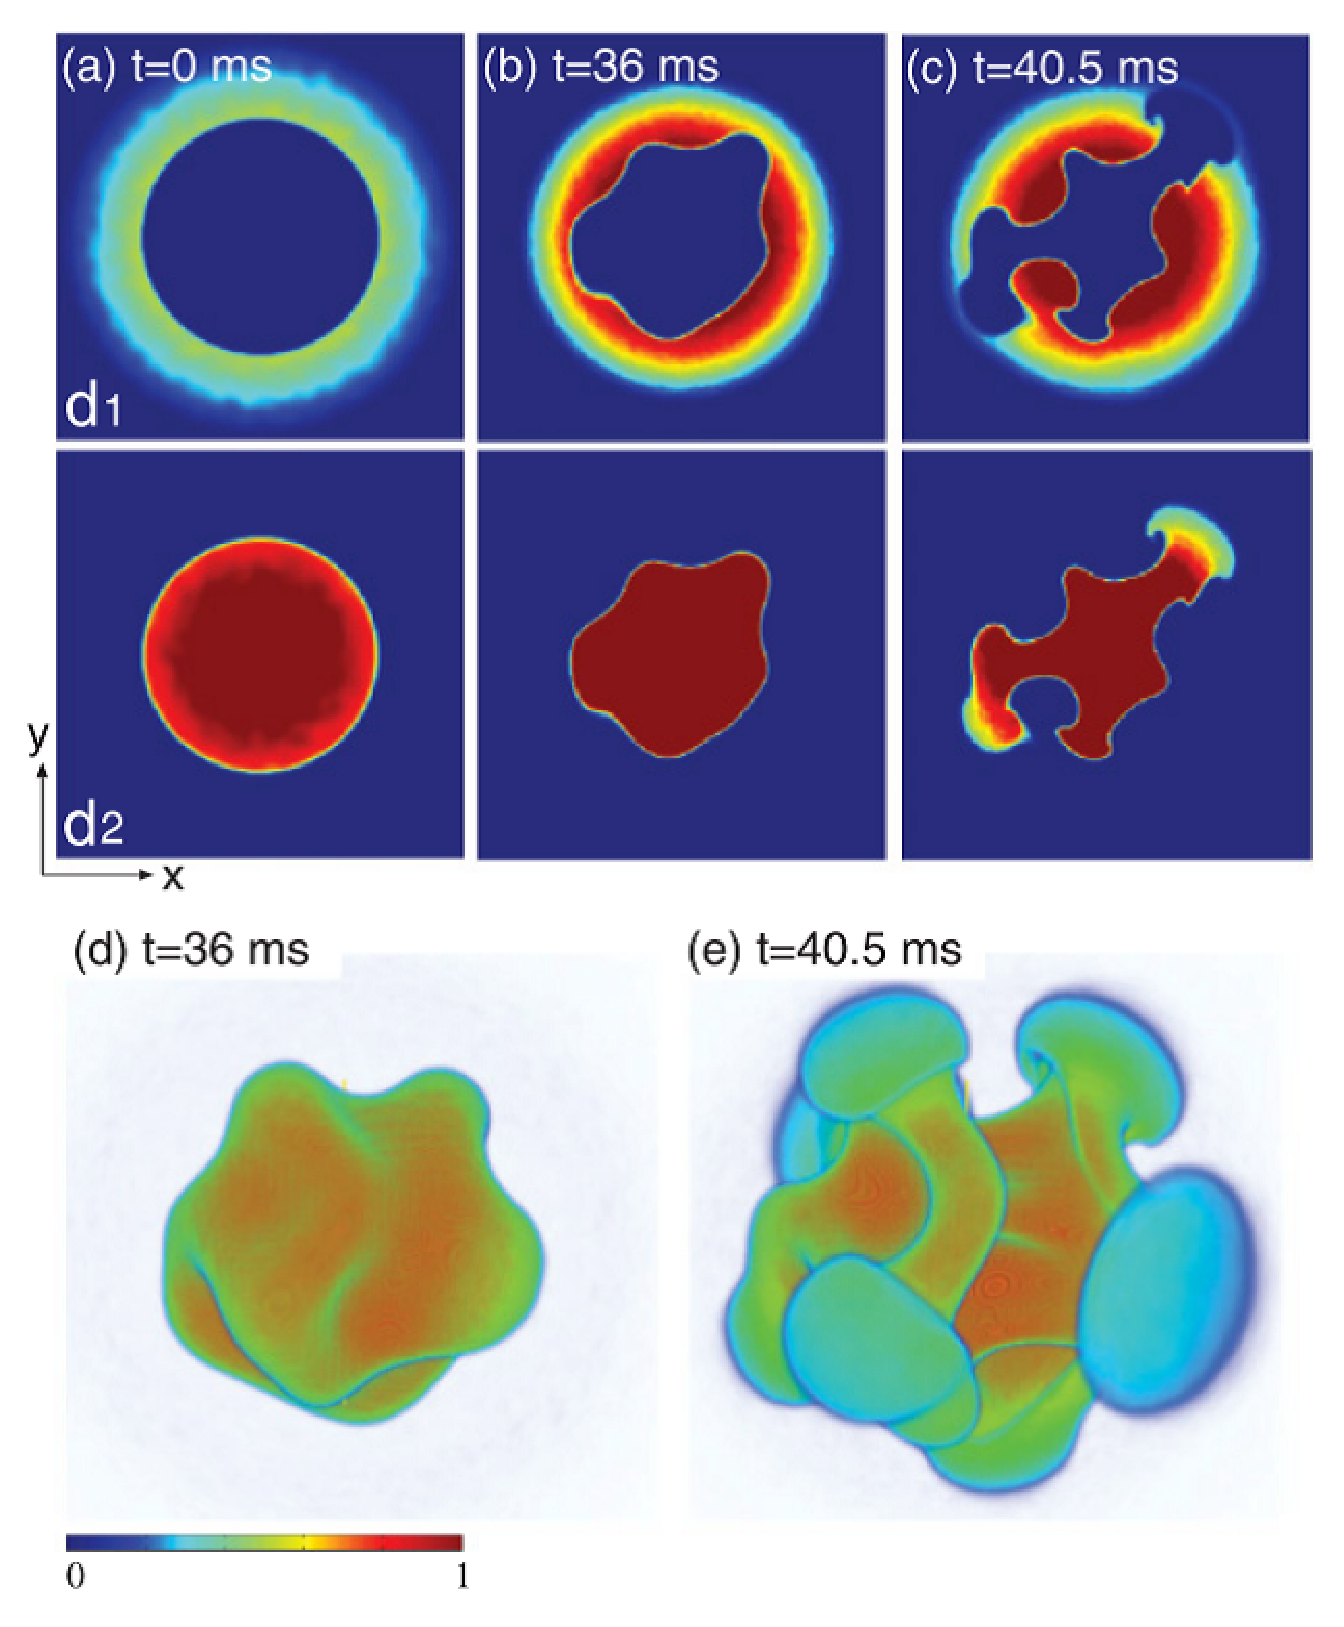
\includegraphics[scale=0.5,keepaspectratio]{5-3.eps}
\caption{(a)-(c) Dynamics of the cross-sectional
density profiles $d_1 = | \psi_1 (z=0) |^2$ and $d_2 = | \psi_2 (z=0) |^2$ of components
one and two and (d), (e) the isodensity surfaces of component
two in a spherically symmetric trap with frequency $\omega_1(t=0)= \omega_2 = 2 \pi \times 33.3 $ Hz.
The trap frequency $\omega_1$ is increased such that $\omega_1^2$
is linearly increased from $(\omega_1 / \omega2)^2 = 1$ to $3$ between $t=0$ and
$t=30$ ms, and after that $(\omega_1/\omega_2)^2$ is fixed to $3$. The scattering length
of component one is $a_{11} = 200_{a_B}$ , and the numbers of atoms are
$N_1 = N_2 = 5.2 \times 10^6$. The unit of the density is $3.0 \times 10^{14}$ cm$^{-3}$.
The field of view of each panel is $56.6 \times 56.6$ $\mu$m.}
\label{FIG:5-3}
\end{center}
\end{figure}

\subsection{Bogoliubov analysis}
\ For a more precise understanding of the instability, we perform a
Bogoliubov analysis for spherically symmetric trap. We expand the
GP equation in Eq.(5.1) up to the first order of the deviation $\delta \psi_j (\vec{r})$
from the meta-stable state $\psi_j(r)$ with spherical symmetry. The excitation mode of the form
\begin{eqnarray}
\delta \psi_j & = & u_j(r)Y_l^m(\theta, \phi)e^{-i \Omega t} + v_j^* (r)Y_l^{m*}(\theta, \phi)e^{i \Omega t}
\end{eqnarray}
obeys the Bogoliubov-de Gennes equations $(j \neq j^\prime)$
\begin{subequations}
\begin{align}
\left(K_{jl} + V_j - \mu_j + 2g_{jj} \Psi^2_j + g_{jj^\prime} \Psi^2_{j^\prime} \right) u_j
+ g_{jj} \Psi^2_j v_j + g_{jj^\prime} \Psi_j \Psi_{j^\prime} (u_{j^\prime} + v_{j^\prime})
& = \hbar \Omega u_j,
\\
\left(K_{jl} + V_j - \mu_j + 2g_{jj} \Psi^2_j + g_{jj^\prime} \Psi^2_{j^\prime} \right) v_j
+ g_{jj} \Psi^2_j u_j + g_{jj^\prime} \Psi_j \Psi_{j^\prime} (u_{j^\prime} + v_{j^\prime})
& = \hbar \Omega v_j,
\end{align}
\end{subequations}
where $\mu_j$ is the chemical potential and
\begin{eqnarray}
K_{jl} & = & - \frac{\hbar^2}{2m_j} \left[ \frac{\diff^2}{\diff r^2} + \frac{2}{r} \frac{\diff}{\diff r}
- \frac{l(l+1)}{r^2} \right]
\end{eqnarray}
The wave function $\Psi_j$ is assumed to be real without loss of
generality. We numerically diagonalize Eq.(4) to study the
stability of the system. If there is a complex frequency $Omega$,
the corresponding mode grows exponentially, and the system
is dynamically unstable. Figure 5.4 shows the imaginary part
of the Bogoliubov excitation frequency Im$\Omega$ as a function
of $(\omega_1 / \omega_2)^2$. The critical value of $(\omega_1 / \omega_2)^2$ above which
Im$\Omega$ rises increases with an increase in $l$. and above this
critical value of $(\omega_1 / \omega_2)^2$, Im$\Omega$ monotonically increases At
$(\omega_1 / \omega_2)^2 = 3$ (the vertical line in Fig. 5.4), which corresponds
to the parameter in Fig. 5.3, the modes of $l=1-10$ are unstable.
Among these modes, the mode which has the largest Im$\Omega$
dominates the unstable dynamics. In Fig. 5.4, since Im$\Omega$ of the
$l=5-7$ modes are all comparably large, these modes will
dominate the unstable dynamics. For these parameters, the
analytic expression in Eq.(2) estimates that the modes of $l=1-7$
are unstable whereas the modes of $l=1-10$ are unstable
in Fig. 5.4. The difference is attributed to the assumptions of
incompressibility and inhomogeneous density distribution in
Eq.(2) and the ambiguity in the inter-facial-tension coefficient
$\sigma$ for a trapped system.
\begin{figure}[htbp]
\begin{center}
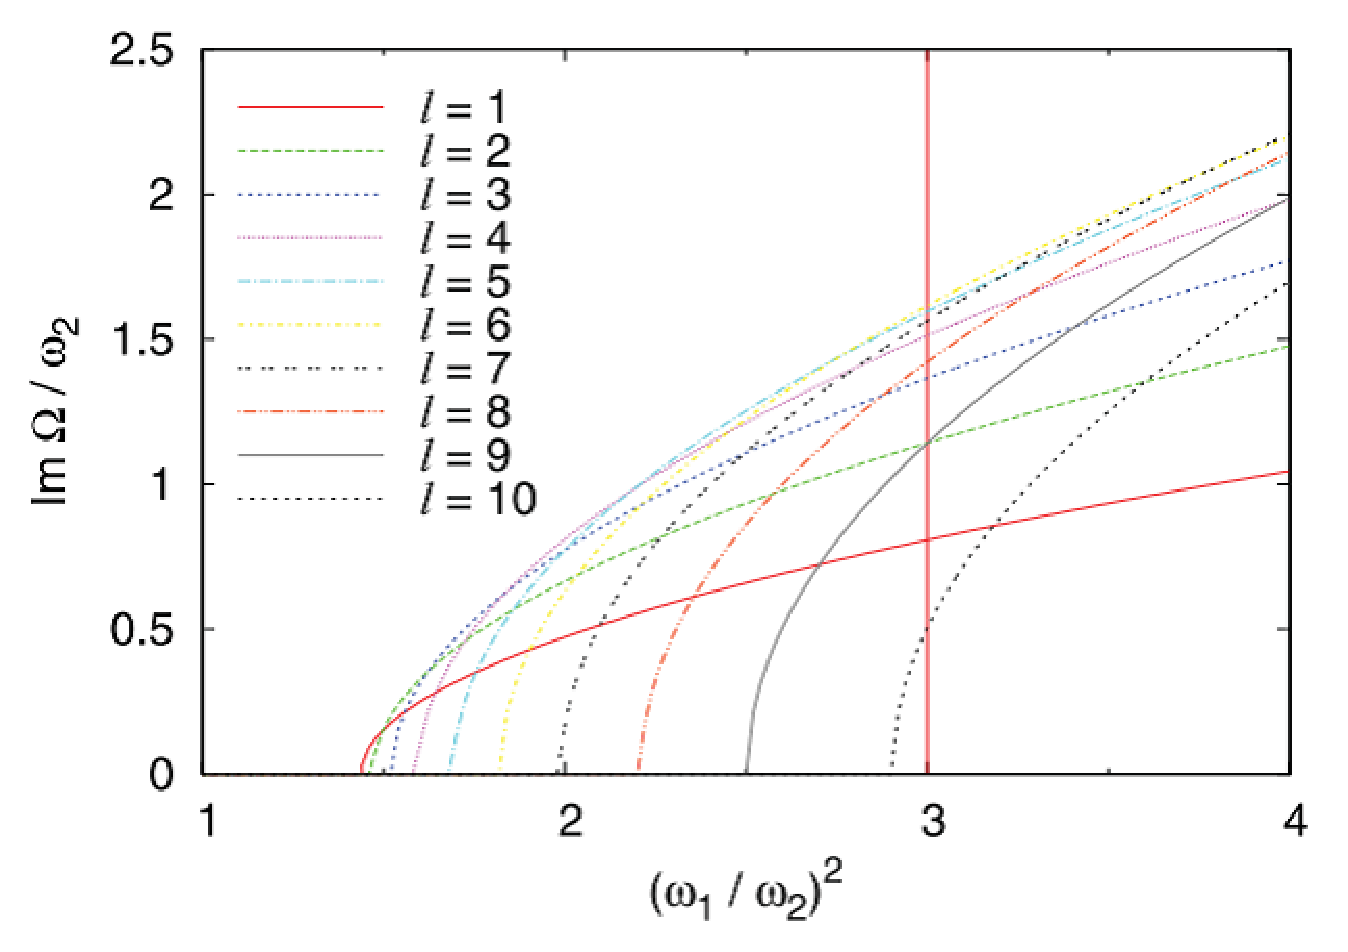
\includegraphics[scale=0.50,keepaspectratio]{5-4.eps}
\caption{
Imaginary part of the Bogoliubov excitation
frequency Im as a function of $( \omega 1 / \omega 2 )^2$. The parameters
are the same as those in FIG. 5.3. The modes for {\it l} $\le 10$ are plotted,
where l is define in Eq. (5.3). The vertical line indicates $( \omega 1 / \omega 2 )^2 = 3$,
corresponding to the parameter in Fig. 5.3.
}
\label{FIG:5-4}
\end{center}
\end{figure}

\section{Conclusion}
\ In conclusion, we have investigated the interfacial instabilities
and subsequent dynamics in phase-separated two-component
BECs. Since the initial state has rotational symmetry,
the symmetry-breaking nature of the RTI can specifically
be observed in this system. We have demonstrated the RTI and
ensuing dynamics for an axisymmetric oblate trap (Figs.5.1 and 5.2)
and a spherically symmetric trap Fig. 5.3, and the
mushroom-shaped patterns are observed for both systems,
breaking the rotational symmetry. We performed a Bogoliubov
analysis for the spherically symmetric system and obtained an
unstable spectrum Fig. 5.4.
\\
\ In view of the recent development in the control of
two-component BECs \cite{72}\cite{75}\cite{76},we expect that not only the
phenomena predicted in the present chapter but also other
theoretical predictions \cite{62}\cite{63}\cite{64}\cite{65}\cite{77}\cite{78}\cite{79}\cite{80}
concerning interfacial instabilities in
two-component BECs will be realized in experiments in the near future.
\if 0
%A2BECRTI邱B
%2AQIB
%sA^E[hqQ
%AT邱B
\ It turned out that the phenomenon of RTI is seen
of also axial symmetry and spherical symmetry.
Moreover, the number of the vortex rings
which occur by the rate of two components
in axial symmetry is unique.
And in spherical symmetry,
instability analysis showed
that the mode of the interface
to give and the number of the quantized vortex rings corresponded,
and it was similar to the thing of classic fluid.
%SqiBECjATlRTI
%BSp[^_IfA
%gbvnAlqBECp
%\邱B
Also in quantum fluid (BEC) without viscosity,
the phenomenon of the RTI same as classical fluid,
such as water and oil, was shown.
It has suggested that the experiment
with high reproducibility using BEC
which it is easy to carry out theoretical modeling,
and is characterized by a uniform quantum state
n the trap system of axial symmetry
or spherical symmetry from not having a parameter
called viscosity is possible.
\fi

\chapter*{Acknowledgements}
\ I would like to express my sincere thanks to Professor Hiroki Saito for
giving me to opportunity of working at The University of Electro-Communications
for advanced study and for his kind interest in this work.
And I am much thankful to my wife Chie, my parents, our laboratory member and two dogs Bonnie, Yuki who had followed
warmly until this study completed. Let it go, the cold never bothered me anyway. \cite{81}.

% \chapter*{References}
\begin{thebibliography}{81}
%\begin{document}
\bibitem[1]{1} S.N.Bose, Z. {\em Phys.} {\bf 26}, (1924) 178.
\bibitem[2]{2} A.Einstein ,Sitzungsberg K.Preuss. Akad. Wiss., Phys. Math. {\bf K1}. No.22, 261(1924); No. 1,3(1925)
\bibitem[3]{3} Anderson M. H., J.R. Ensher, M.R.Matthews, C.E.Wieman, E.A.Cornell, Science {\bf 269}, (1995) 198.
\bibitem[4]{4} Davis K.B., M.O.Mewes, M.R.Andrews, N.J.von Druten, D.F.Durfee, D.M.Kurn, W.Ketterle, Phys. Rev Lett. {\bf 75}, (1995) 3969.
\bibitem[5]{5} W.H.Keesom and K.Clusius, Leiden Comm. 219e(1932). [Proc. Sect. Sci. K. Ned. Acad. Wet. {\bf 35}, 307 (1932)].
\bibitem[6]{6} P.Kapitza, {\em Nature} {\bf 141} 74 (1938)
\bibitem[7]{7} F.London, {\em Nature} {\bf 141}, 643(1938)
\bibitem[8]{8} L.P.Pitaevskii, Sov. Phys. JETP {\bf 13}, 451(1961)
\bibitem[9]{9} E.P.Gross, I {\em l Nouvo Cimento} {\bf 20}, 454(1961); {\em J.Math. Phys.} {\bf 4}, 195(1963)
\bibitem[10]{10} E.Cornel and C.Wieman(JILA,US)cooled gas of $^{87} {\rm Rb}$ atoms at $170 {\rm nK}$ (1995)
\bibitem[11]{11} Bradley {\it et al} first observed BEC for $^{7} {\rm Li}$ atoms (1995)
\bibitem[12]{12} W.Ketterle(MIT, US) observed BEC for $^{23} {\rm Na}$ atoms (1995)
\bibitem[13]{13} E.Fermi, "Zur Quantelung des idealen einatomigen Gases," Zeitschrift f\"{u}r Physik {\bf 36} (1926), no. 11-12, p.902-12.
\bibitem[14]{14} P.A.M.Dirac, "On the Theory of Quantum Mechanics," Proceedings of the Royal Society (London) A{\bf 112} (1926), pp.281-305.
\bibitem[15]{15} W.Pauli, " \"{U}ber den Zusammenhang des Abschlusses der Elektronengruppen im Atom mit der Komplexstruktur der Spektren," Z.Physik, {\bf 31}, p.765(1925)
\bibitem[16]{16} C.J.Pethick and H.Smith, {\it Bose-Einstein Condensation in Dilute Gases}, 2nd ed. (Cambridge University Press, Cambridge, 2008).
\bibitem[17]{17} L.Pitaevskii and S.Stringari, {\it Bose-Einstein Condensation}, INTERNATIONAL SERIES OF MONOGRAPHS ON PHYSICS {\bf 116}(CLARENDON PRESS,OXFORD 2003).
\bibitem[18]{18} Y.Yamamoto, {\it Bose-Einstein Condansation and Lasers}, APPPHYS 389, Stanford Univ.(2010)
\bibitem[19]{19} T.Frish, Y.Pomeau, S.Rica, Transition to dissipation in a model of superflow, Phys. Rev. Lett. {\bf 69} 1644(1992).
\bibitem[20]{20} T.Winiecki, J.F.McCann, C.S.Adams, Pressure Drag in Linear and Nonlinear Quantum Fluids, Phys. Rev. Lett. {\bf 82} 5186(1999).
\bibitem[21]{21} T.Winiecki, B.Jackson, J.F.McCann, and C.S.Adams, J.Phys. B {\bf 33}, 4069(2000).
\bibitem[22]{22} C.Nore, C.Huepe, and M.E.Brachet, Phys.Rev.Lett. {\bf 84}, 2191(2000).
\bibitem[23]{23} A.Aftalion, Q.Du, and Y.Pomeau, Phys. Rev. Lett. {\bf 91}, 090407(2003).
\bibitem[24]{24} J.S.Stie\ss berger, W.Zwerger, Critical velocity of superfluid flow past large obstacles in Bose-Einstein condensates, Phys. Rev. A {\bf 62} (2000)061601(R).
\bibitem[25]{25} C.Huepe and M.E.Brachet, Physica(Amsterdam) {\bf 140D}, 126(2000).
\bibitem[26]{26} G.A.El, A.Gammal, and A.M.Kamchatnov, Phys. Rev. Lett. {\bf 97}, 180405(2006).
\bibitem[27]{27} I.Carusotto, S.X.Hu, L.A.Collins, and A.Smerzi, Phys. Rev. Lett. {\bf 97}, 260403(2006).
\bibitem[28]{28} H.Susanto, P.G.Kevrekidis, R.Carretero-Gonz$\acute{a}$lez, B.A.Malomed, D.J.Frantzeskakis, and A.R.Bishop, Phys. Rev. A {\bf 75}, 055601(2007).
\bibitem[29]{29} A.S.Rodrigues, P.G.Kevrekidis, R.Carretero-Gonz$\acute{a}$lez, D.J.Frantzeskakis, P.Sshmelcher, T.J.Alexander, and Yu.S.Kivshar, Phys. Rev. A {\bf 79}, 043603(2009).
\bibitem[30]{30} Hydrodynamic generation of vortex pairs in a Bose-Einstein condensate is reported in T.W.Neely, E.C.Samson, A.S.Bradley, M.J.Davis, B.P.Anderson, Observation of Vortex Dipoles in an Oblate Bose-Einstein Condensate, Phys. Rev. Lett. {\bf 104} (2010)160401.
\bibitem[31]{31} H.Saito, T.Aioi and T.Kadokura, B$\acute{e}$nard-von K$\acute{a}$rm$\acute{a}$n vortex street in an exiton-polariton superfluid, Phys. Rev. B{\bf 86}, 014504(2012).
\bibitem[32]{32} For recent review of exciton-polariton superfluids, see, I.Carusotto, C.Ciuti, Quantum fluids of light, Rev.Mod.Phys.{\bf 85} (2013)299.
\bibitem[33]{33} T.Aioi, T.Kadokura, T.Kishimoto, and H.Saito, Controlled generation and manipulation of vortex dipoles in a Bose-Einstein condensate, Phys Rev. X{\bf 1}, 021003(2011).
\bibitem[34]{34} W.H.Press, S.A.Teukolsky, W.T.Vetterling, and B.P.Flannery, {\it Numerical Recipes}, 3rd ed, Sec. 20.7 (Cambridge Univ. Press, Cambridge, 2007).
\bibitem[35]{35} S.Rica, A remark on the critical speed of vortex nucleation in the nonlinear Schr\"{o}dinger equation, Physica D{\bf 148}, 221(2001).
\bibitem[36]{36} J.Zhang, S.Childress, A.Libchaber, and M.Shelley, Nature(London) {\bf 408}, 835(2000).
\bibitem[37]{37} M.Shelley, N.Vandenberghe, and J.Zhang, Phys. Rev. Lett. {\bf 94}, 094302(2005).
\bibitem[38]{38} R.E.D.Bishop and A.Y.Hassan, Proc. Roy. Soc. Lond. A {\bf 277}, 51(1964).
\bibitem[39]{39} M.M.Zdravkovich, J.Fluids Eng. {\bf 99}, 618(1977).
\bibitem[40]{40} C.H.K. Williamson, Annu. Rev. Fluid Mech. {\bf 28}, 477(1996).
\bibitem[41]{41} V.K.Horv$\acute{a}$th, J.R.Cressman, W.I.Goldburg, and X.L.Wu, Phys. Rev. E {\bf 61}, R4702(2000).
\bibitem[42]{42} T.B.Benjamin, Prod. R. Soc. Lond. A {\bf 359}, 1 (1978); {\it ibid}, {\bf 359}, 27(1978).
\bibitem[43]{43} H.Kojima, W.Veith, S.J.Putterman, E.Guyon, and I.Rudnick, Phys. Rev. Lett. {\bf 27}, 714(1971).
\bibitem[44]{44} S.Eckel, J.G.Lee, F.Jendrzejewski, N.Murray, C.W.Clark, C.J.Lobb, W.D.Phillips, M.Edwards, and G.K.Campbell, Nature(London) {\bf 506}, 200(2014)
\bibitem[45]{45} C.Raman, M.K\"{o}hl, R.Onofrio, D.S.Durfee, C.E.Kuklewicz, Z.Hadzibabic, and W.Ketterle, Phys. Rev. Lett. {\bf 83}, 2502(1999).
\bibitem[46]{46} R.Onofrio, C.Raman, J.M.Vogels, J.R.Abo-Shaeer, A.P.Chikkatur, and W.Ketterle, Phys. Rev. Lett. {\bf 85}, 2228(2000).
\bibitem[47]{47} C.Nore, M.E.Brachet, and S.Fauve, Physica D {\bf 65}, 154(1993).
\bibitem[48]{48} B.Jackson, J.F.McCann, C.S.Adams, Vortex Formation in Dilute Inhomogeneous Bose-Einstein Condensates, Phys. Rev. Lett. {\bf 80} 3903(1998).
\bibitem[49]{49} C.Josserand, Y.Pomeau, and S.Rica, Physica D {\bf 134}, 111(1999).
\bibitem[50]{50} C.Heupe, M.E.Brachet, Scaling laws for vortical nucleation solutions in a model of superflow, Physica D {\bf 140} 126(2000).
\bibitem[51]{51} A.Aftalion, Q.Du, Y.Pomeau, Dissipative Flow and Vortex Shedding in the Painlev$\acute{e}$ Boundary Layer of a Bose-Einstein Condensate, Phys. Rev. Lett. {\bf 91} 090407(2003).
\bibitem[52]{52} K.Sasaki, N.Suzuki, and H.Saito, B$\acute{e}$nard-von K$\acute{a}$rm$\acute{a}$n vortex street in a Bose-Einstein condensate, Phys. Rev. Lett. {\bf 104}, 150404(2010)
\bibitem[53]{53} F.Pinsker and N.G.Berloff, arXiv:1401.1517.
\bibitem[54]{54} G.W.Stagg, N.G.Parker, and C.F.Barenghi,arXiv:1401.4041.
\bibitem[55]{55} F.Dalfovo and S.Stringari, Phys. Rev. A {\bf 53}, 2477(1996).
\bibitem[56]{56} H.Lamb, {\it Hydrodynamics}, 6th ed, Sec. 155 (Dover, New York, 1945).
\bibitem[57]{57} L.E.Sadler, J.M.Higbie, S.R.Leslie, M.Vengalattore, and D.M.Stamper-Kurn, Nature(London) {\bf 443}, 312(2006).
\bibitem[58]{58} Lord Rayleigh, Proc. London Math. Soc. {\bf 14}, 170(1883).
\bibitem[59]{59} G.I.Taylor, Proc. R. Soc. London, Ser. A {\bf 201}, 192(1950).
\bibitem[60]{60} D.J.Lewis, Proc.R.Soc. London, Ser. A {\bf 202}, 81(1950).
\bibitem[61]{61} For example, see S.Chandrasekhar, {\it Hydrodynamic and Hydromagnetic Stability} (Clarendon Press, Oxford, 1961), Chap. 10.
\bibitem[62]{62} K.Sasaki, N.Suzuki, D.Akamatsu, and H.Saito, Phys. Rev. A {\bf 80}, 063611(2009).
\bibitem[63]{63} S.Gautam and D.Angom, Phys. Rev. A {\bf 81}, 053616 (2010).
\bibitem[64]{64} A.Bezett, V.Bychkov, E.Lundh, D.Kobyakov, and M.Marklund, Phys. Rev. A {\bf 82}, 043608(2010).
\bibitem[65]{65} D.Kobyakov, V.Bychkov, E.Lundh, A.Bezett, V.Akkerman, and M.Marklund, Phys. Rev. A {\bf 83}, 043623(2011).
\bibitem[66]{66} A.Burrows, Nature (London) {\bf 403}, 727(2000).
\bibitem[67]{67} V.Bychkov, M.V.Popov, A.M. Oparin, L.Stenflo, and V.M. Chechetkin, Astron. Rep. {\bf 50}, 298(2006).
\bibitem[68]{68} W.H.Cabot and A.W.Cook, Nat. Phys. {\bf 2}, 562(2006).
\bibitem[69]{69} H.Sakagami and K.Nishihara, Phys. Rev. Lett. {\bf 65}, 432(1990).
\bibitem[70]{70} M.S.Plesset, J.Appl. Phys. {\bf 25}, 96(1954).
\bibitem[71]{71} M.P.Brenner, D.Lohse, and T.F.Dupont, Phys. Rev. Lett. {\bf 75}, 954(1995).
\bibitem[72]{72} S.B.Papp, J.M.Pino, and C.E.Wieman, Phys. Rev. Lett. {\bf 101}, 040402(2008).
\bibitem[73]{73} H.Lamb, {\it Hydrodynamics}, 6th ed, Sec. 275 (Dover, New York, 1945).
\bibitem[74]{74} B.Van Schaeybroeck, Phys. Rev. A {\bf 78}, 023624(2008); {\bf 80},065601(2009).
\bibitem[75]{75} K.M.Mertes, J.W.Merrill, R.Carretero-Gonz$\acute{a}$lez, D.J. Frantzeskakis, P.G.Kevrekidis, and D.S.Hall, Phys. Rev. Lett. {\bf 99}, 190402(2007).
\bibitem[76]{76} S.Tojo, Y.Taguchi, Y.Masuyama, T.Hayashi, H.Saito, and T.Hirano, Phys. Rev. A {\bf 82}, 033609(2010).
\bibitem[77]{77} H.Saito, Y.Kawaguchi, and M.Ueda, Phys. Rev. Lett. {\bf 102}, 230403(2009).
\bibitem[78]{78} H.Takeuchi, N.Suzuki, K.Kasamatsu, H.Saito, and M.Tsubota, Phys. Rev. B {\bf 81}, 094517(2010).
\bibitem[79]{79} N.Suzuki, H.Takeuchi, K.Kasamatsu, M.Tsubota, and H.Saito, Phys. Rev. A {\bf 82}, 063604(2010).
\bibitem[80]{80} K.Sasaki, N.Suzuki, and H.Saito, Phys. Rev. A {\bf 83}, 053606(2011).
\bibitem[81]{81} Walt Disney Studios Motion pictures {\it Frozen}, El Capitan Theatre(2013).
\end{thebibliography}
%\end{document}
\newpage
\
\\
Related Study Papers
\\
\\
Hysteresis in quantized vortex shedding
\\
Tsuyoshi Kadokura, Jun Yoshida, and Hiroki Saito
\\
Physical Review A {\bf 90}, 013612 (2014)
\\
arXiv:1405.4577
\\
\\
Dissipative structures of quantized vortices in a coherently pumped polariton superfluid
\\
Tomohiko Aioi, Tsuyoshi Kadokura, and Hiroki Saito
\\
Physical Review B {\bf 87}, 205312 (2013)
\\
arXiv:1302.4846
\\
\\
Order-disorder oscillations in exciton-polariton superfluids
\\
Hiroki Saito, Tomohiko Aioi, and Tsuyoshi Kadokura
\\
Physical Review Letters {\bf 110}, 026401 (2013)
\\
arXiv:1208.4886
\\
\\
Benard-von Karman vortex street in an exciton-polariton superfluid
\\
Hiroki Saito, Tomohiko Aioi, and Tsuyoshi Kadokura
\\
Physical Review B {\bf 86}, 014504 (2012)
\\
arXiv:1205.1611
\\
\\
Penetration of a vortex dipole across an interface of Bose-Einstein condensates
\\
Tomohiko Aioi, Tsuyoshi Kadokura, and Hiroki Saito
\\
Physical Review A {\bf 85}, 023618 (2012)
\\
arXiv:1112.4028
\\
\\
Rayleigh-Taylor instability in a two-component Bose-Einstein condensate
\\
with rotational symmetry
\\
Tsuyoshi Kadokura, Tomohiko Aioi, Kazuki Sasaki, Tetsuo Kishimoto, and Hiroki Saito
\\
Physical Review A {\bf 85}, 013602 (2012)
\\
\\
Symmetry breaking Rayleigh-Taylor instability in a two-component Bose-Einstein condensate
\\
Tsuyoshi Kadokura, Tomohiko Aioi, Kazuki Sasaki, Tetsuo Kishimoto, Hiroki Saito
\\
arXiv:1111.1283 (5 Nov 2011)
\\
\\
Controlled generation and manipulation of vortex dipoles in a Bose-Einstein condensate
\\
Tomohiko Aioi, Tsuyoshi Kadokura, Tetsuo Kishimoto, and Hiroki Saito
\\
Physical Review X {\bf 1}, 021003 (2011)
\\
arXiv:1106.1314
\newpage
\
\\
Conference presentation
\\
\\
Hysteresis in quantized vortex shedding
\\
8pAW-7, 2014 Autumn Meeting, Chubu University, The Physical Society of Japan (JPS)
\\
\\
Reyleigh-Taylor instability in a two-component Bose-Einstein condensate
\\
with rotational symmetry
\\
25aBE-11, 2012 Annual (67th) Meeting, KWANSEI GAKUIN University,
\\
The Physical Society of Japan (JPS)

\begin{flushright}
\LaTeX \\
\end{flushright}
\end{document}
%eof
